\documentclass{greaseproof}
\usepackage{lipsum}

\usepackage{tikz}
\usetikzlibrary{calc}

\newcommand{\loremipsum}{ {\color{gray}  Lorem ipsum dolor sit amet, consectetur adipiscing elit. Suspendisse nisl purus, ultricies et ante quis, iaculis imperdiet justo. Proin tristique turpis a tortor eleifend lobortis. Vestibulum odio nisi, tempor sed scelerisque ac, aliquet a lorem. Proin ullamcorper nibh eget augue placerat lobortis. Quisque ac commodo libero, fringilla dictum purus. Proin nec massa vitae lorem eleifend lacinia. Praesent rhoncus ultricies ullamcorper. Fusce vel viverra purus, nec rhoncus massa. Etiam nisl lorem, cursus vel est sit amet, mattis venenatis magna. Vestibulum id risus sit amet nisi congue ultrices id nec ex. } }
\newcommand{\todofoot}[1]{\textcolor{red}{\textbf{(!)}\footnote{\textbf{\color{red}{Do zrobienia}}: #1}}}

\begin{document}

% strona pierwsza
\thispagestyle{empty}
{\noindent\fontsize{18pt}{18pt}\selectfont Biblioteka Aleksandryjska, tom I}

\noindent\makebox[\linewidth]{\rule{\textwidth}{1pt}}

\newpage

% strona druga
\thispagestyle{empty}
\phantom{nothing}
\newpage

% strona trzecia
\thispagestyle{empty}
{\noindent\fontsize{18pt}{18pt}\selectfont Epafrodyt z Ptolemais}

\noindent\makebox[\linewidth]{\rule{\textwidth}{1pt}}

\vspace{10mm}

{\noindent\fontsize{24pt}{24pt}\selectfont \textbf{Geometria}}
\vspace{10mm}

{\noindent\fontsize{14pt}{14pt}\selectfont Wydanie zerowe (eksperymentalne)}

\newpage

% strona czwarta
\thispagestyle{empty}
\begin{figure}[H]
\begin{minipage}[b]{.48\linewidth}
{\noindent Epafrodyt z Eudoksos\\
do napisania\\
do napisania\\
do napisania}
\end{minipage}
\begin{minipage}[b]{.48\linewidth}
{\noindent do napisania\\
do napisania\\
do napisania\\
do napisania}
\end{minipage}
\end{figure}

{\noindent \textbf{Kategorie MSC 2020}\\do napisania} \vspace{5mm}

{\noindent \textbf{Tytuł oryginału}\\do napisania} \vspace{5mm}

{\noindent \textbf{Z greki tłumaczyła}\\do napisania} \vspace{5mm}

{\noindent \textbf{Okładkę zaprojektował}\\do napisania} \vspace{5mm}

{\noindent \textbf{Zredagował}\\do napisania} \vspace{5mm}

{\noindent \textbf{Zredagowała technicznie}\\do napisania} \vspace{5mm}

{\noindent \textbf{Złożyli i połamali}\\do napisania} \vspace{5mm}

{\noindent \textbf{Korekty dokonali}\\do napisania} \vfill

{\noindent Copyleft © 2024 by Antykwariat Czarnoksięski.
Książka, a żeby było śmieszniej także każda jej część, mogą być przedrukowywane oraz w jakikolwiek inny sposób reprodukowane czy powielane mechanicznie, fotooptycznie, zapisywane elektronicznie lub magnetycznie, oraz odczytywane w środkach publicznego przekazu bez pisemnej zgody wydawcy.
}

\vspace{5mm}
{
    \noindent
    Tekst udostępniany na licencji Creative Commons: uznanie autorstwa, użycie niekomercyjne. Przeczytaj więcej na \texttt{https://creativecommons.org/licenses/by-nc/4.0/deed.pl}.
}

\vspace{5mm}

{\noindent Przygotowano w systemie \TeX, wydrukowano na siarczystym papierze.}

% strona piąta
\newpage
\section*{Przedmowa}
Do napisania.

\begin{flushright}
Epafrodyt,\\gdzie, kiedy
\end{flushright}

\tableofcontents
% \pagestyle{fancy} % Enable default headers and footers again
\cleardoublepage % Start the following content on a new page

% section 1
\section{Aksjomatyka}
Tekst podsekcji Aksjomatyka. \loremipsum
%

\section{Aksjomaty Euklidesa}
\todofoot{Considered the "father of geometry",[3] he is chiefly known for the Elements treatise, which established the foundations of geometry that largely dominated the field until the early 19th century.}
\todofoot{Very little is known of Euclid's life, and most information comes from the scholars Proclus and Pappus of Alexandria many centuries later. }

\todofoot{The theorem of the gnomon was described as early as in Euclid's Elements (around 300 BC), and there it plays an important role in the derivation of other theorems. It is given as proposition 43 in Book I of the Elements, where it is phrased as a statement about parallelograms without using the term "gnomon". The latter is introduced by Euclid as the second definition of the second book of Elements. Further theorems for which the gnomon and its properties play an important role are proposition 6 in Book II, proposition 29 in Book VI and propositions 1 to 4 in Book XIII.[5][4][6]} % https://en.wikipedia.org/wiki/Theorem_of_the_gnomon
\todofoot{Strona ,,Euclidean geometry'' na en-wiki} % https://en.wikipedia.org/wiki/Euclidean_geometry

\subsection{Księga I}	
\subsubsection{Definicje}	
\begin{enumerate}	
    \item [1.1] Definicja ... % Definicja 1. % Punkt to jest to, co nie składa się z części.
    \item [1.2] Definicja ... % Definicja 2. % Linia jest długością bez szerokości.
    \item [1.3] Definicja ... % Definicja 3. % Końcami linii są punkty.
    \item [1.4] Definicja ... % Definicja 4. % Linia jest prosta, jeżeli położona jest między swoimi punktami w równym i jednostajnym kierunku.
    \item [1.5] Definicja ... % Definicja 5. % Powierzchnia jest to, co ma tylko długość i szerokość.
    \item [1.6] Definicja ... % Definicja 6. % Krawędzie powierzchni są liniami.
    \item [1.7] Definicja ... % Definicja 7. % Płaska powierzchnia albo płaszczyzna jest ta, na której biorąc gdziekolwiek dwa punkty linia prosta między tymi punktami cała leży na tej powierzchni.
    \item [1.8] Definicja ... % Definicja 8. % Kąt płaski to nachylenie dwóch linii na płaszczyźnie w miejscu, w którym jedna spotyka drugą i nie leżą w linii prostej.
    \item [1.9] Definicja ... % Definicja 9. % Kiedy linie są proste i tworzą kąt, wtedy kąt zwany jest prostoliniowym.
    \item [1.10] Definicja ... % Definicja 10. % Kiedy linia prosta padająca na drugą linie prostą, tworzy z nią kąty przyległe równe między sobą, to każdy z kątów równych nazywamy prostym, a padająca linia prostą nazywa się prostopadłą do tej linii, na którą pada.
    \item [1.11] Definicja ... % Definicja 11. % Kąt rozwarty jest większy od kąta prostego.
    \item [1.12] Definicja ... % Definicja 12. % Kąt ostry jest mniejszy od kąta prostego.
    \item [1.13] Definicja ... % Definicja 13. % Kresem albo granicą jest to, na czym się dana rzecz kończy.
    \item [1.14] Definicja ... % Definicja 14. % Figurą nazywamy to co jest ograniczone granicą lub granicami.
    \item [1.15] Definicja ... % Definicja 15. % Koło jest figurą płaską zawarta linią zwaną okręgiem, do której wszystkie linie proste poprowadzone z jednego punktu wewnątrz figury położonego, są między sobą równe.
    \item [1.16] Definicja ... % Definicja 16. % I ten punkt nazywa się centrum lub środkiem koła.
    \item [1.17] Definicja ... % Definicja 17. % Średnicą koła jest każda linia narysowana przez środek koła, przedłużona w dwóch kierunkach do jego obwodu, przepoławiająca go.
    \item [1.18] Definicja ... % Definicja 18. % Półokręgiem jest figura zawarta między średnicą i częscia okręgu odciętą tą średnicą. Środek półokregu jest też środkiem okręgu.
    \item [1.19] Definicja ... % Definicja 19. % Figury prostokreślne to figury ograniczone prostymi. Trójkąt to figura prostokreślna ograniczona trzema prostymi. Czworobok lub czworokąt to figura prostokreślna, która jest ograniczona czterema prostymi. Wielobok lub wielokąt to figura prostokreślna ograniczona więcej niż czterema prostymi.
    \item [1.20] Definicja ... % Definicja 20. % Trójkąt równoboczny to trójkąt, który ma trzy boki równe. Trójkąt równoramienny to trójkąt, który ma tylko dwa boki równe. Trójkąt różnoboczny to trójkąt, który ma trzy boki różne.
    \item [1.21] Definicja ... % Definicja 21. % Ponadto: trójkąt prostokątny to trójkąt, który na kąt prosty. Trójkąt rozwartokątny to trójkąt, który ma kąt rozwarty. Trójkąt ostrokątny to trójkąt, który ma trzy kąty ostre.
    \item [1.22] Definicja ... % Definicja 22. % Kwadrat jest to czworobok mający równe boki i równe kąty. Prostokąt jest to czworobok mający kąty proste, ale boki nierówne. Romb (kwadrat ukośny) jest to czworobok mający równe boki, ale nie mający kątów prostych. Równoległobok jest to czworobok mający boki przeciwległe równe, ale nie mający katów prostych. Wszystkie czworoboki inne niż wyżej wymienione nazywamy czworokątami.
    \item [1.23] Definicja ... % Definicja 23. % Linie równoległe, czyli mówiąc krócej równoległe są to proste, które leżą na tej samej płaszczyźnie i przedłużone z obu stron w nieskończoność, z żadnej strony nie przetną się.
\end{enumerate}	
	
\subsubsection{Postulaty}	
\begin{enumerate}	
    \item [1.1] Postulat ... % Postulat 1 % Można poprowadzić prostą od któregokolwiek punktu do któregokolwiek punktu.
    \item [1.2] Postulat ... % Postulat 2. % Ograniczoną prostą można przedłużyć nieskończenie.
    \item [1.3] Postulat ... % Postulat 3. % Można zakreślić okrąg z któregokolwiek punktu jako środka dowolną odległością.
    \item [1.4] Postulat ... % Postulat 4. % Wszystkie kąty proste są między sobą równe.
    \item [1.5] Postulat ... % Postulat 5. % Jeżeli prosta przecinająca dwie proste tworzy z nimi kąty jednostronnie wewnętrzne o sumie mniejszej niż dwa kąty proste, to te dwie proste przedłużone nieskończenie przecinają się po tej stronie, po której znajdują się kąty o sumie mniejszej od dwóch kątów prostych.
\end{enumerate}	
	
Jak łatwo zauważyć, sformułowanie ostatniego postulatu używa więcej słów niż pozostałe razem wzięte; wbrew przekonaniu, że postulaty miały wyrażać treści oczywiste i proste.	
Piąty postulat wydawał się bardziej skomplikowany, więc nasuwał podejrzenie, że wynika z poprzednich czterech.	
Zauważył to już Proklos (410-485): \emph{,,Nie jest możliwe, aby uczony tej miary co Euklides godził się na obecność tak długiego postulatu w aksjomatyce -- obecność postulatu wzięła się z pospiesznego kończenia przez niego Elementów, tak aby zdążyć przed nadejściem słusznie oczekiwanej rychłej śmierci; my zatem -- czcząc jego pamięć -- powinniśmy ten postulat usunąć lub co najmniej znacznie uprościć.''}	
	
Wiele osób próbowało stawić czoło wyzwaniu postawionemu przez Proklosa.	
Było to bezskuteczne, ponieważ piąty postulat jest niezależny od pozostałych, zaś zastąpienie go jego zaprzeczeniem prowadzi do geometrii nieeuklidesowych.	
Piszą o nim Audin \cite[s. 13]{audin_2003}.
	
\subsubsection{Pojęcia pierwotne}	
\begin{enumerate}	
    \item [1.1] Pojęcie pierwotne ... % Pojęcie podstawowe 1 % Wyrażenia, które są równe się temu samemu wyrażeniowi, są sobie równe.
    \item [1.2] Pojęcie pierwotne ... % Pojęcie podstawowe 2 % Jeżeli równania dodawane są do równań, wtedy całości są sobie równe.
    \item [1.3] Pojęcie pierwotne ... % Pojęcie podstawowe 3 % Jeżeli równania odejmowane są do równań, wtedy całości są sobie równe.
    \item [1.4] Pojęcie pierwotne ... % Pojęcie podstawowe 4 % Wyrażenia, które się pokrywają, są sobie równe.
    \item [1.5] Pojęcie pierwotne ... % Pojęcie podstawowe 5 % Całość jest większa od części.
\end{enumerate}	
	
\subsubsection{Twierdzenia}	
\begin{enumerate}	
    \item [1.1] Twierdzenie ... % Twierdzenie 1. % Na danej linii prostej skonstruuj trójkąt równoboczny o żadanych bokach.
    \item [1.2] Twierdzenie ... % Twierdzenie 2. % Skonstruuj odcinek równy danemu odcinkowi którego koniec jest zadanym punktem.
    \item [1.3] Twierdzenie ... % Twierdzenie 3. % Mając dane dwie linie proste nierówne, od większej odciąć linię równą mniejszej.
    \item [1.4] Twierdzenie ... \hfill \emph{(przystawanie bok-kąt-bok)} % Twierdzenie 4. % Jeśli dwa trójkąty mają dwa boki odpowiednio równe dwóm innym, i jeżeli kąty zawarte między bokami równoległymi są równe, wtedy ich podstawy również są sobie równe i pozostałe kąty równe są odpowiednim kątom.
    \item [1.5] Twierdzenie ... % Twierdzenie 5. % W trójkątach równoramiennych kąty przy podstawie są sobie równe oraz kąty powstałe przez przedłużenie boków równych są sobie równe.
    \item [1.6] Boki trójkąta leżące naprzeciw przystających kątów są przystające.
    \item [1.7] Twierdzenie ... % Twierdzenie 7. % Na tej samej podstawie i z tej samej strony nie mogą być wykreślone dwa trójkąty takie, żeby boki w tych trójkątach przy obydwu końcach wspólnej podstawy były między sobą równe.
    \item [1.8] Twierdzenie ... \hfill \emph{(przystawanie bok-bok-bok)} % Twierdzenie 8. % Jeżeli dwa boki jednego trójkąta są równe dwóm bokom drugiego trójkąta, to kąty zawarte między równymi bokami są sobie równe.
    \item [1.9] Podzielić dany kąt na dwie równe części.
    \item [1.10] Podzielić dany odcinek na dwie równe części.
    \item [1.11] Twierdzenie ... % Twierdzenie 11. % Z punktu danego na danej linii prostej wyprowadzić linie prostopadłą do danej linii prostej.
    \item [1.12] Twierdzenie ... % Twierdzenie 12. % Z punktu danego leżącego poza linią prostą nieograniczoną, wyprowadzić prostą linię prostopadłą do niej.
    \item [1.13] Twierdzenie ... % Twierdzenie 13. % Jeżeli linia prosta przecinająca drugą prostą tworzy z nią dwa kąty, to są one proste, albo równe dwóm kątom prostym.
    \item [1.14] Twierdzenie ... % Twierdzenie 14. % Jeżeli przy linii prostej i przy punkcie na niej leżącym dwie linie proste nie po jednej stronie położone czynią kąty przyległe równe dwóm kątom prostym, to te linie proste będą w tym samym kierunku.
    \item [1.15] Twierdzenie ... % Twierdzenie 15. % Jeżeli dwie linie proste przecinają się, to utworzone przez nie kąty przeciwległe są sobie równe.
    \item [1.16] Twierdzenie ... % Twierdzenie 16. % W dowolnym trójkącie kąt zewnętrzny powstały przez przedłużenie jednego boku jest większy od każdego z dwóch kątów wewnętrznych przeciwległych jemu.
    \item [1.17] Twierdzenie ... % Twierdzenie 17. % W każdym trójkącie suma dwóch dowolnych kątów jest mniejsza od dwóch kątów prostych.
    \item [1.18] Twierdzenie ... % Twierdzenie 18. % W każdym trójkącie bok większy przeciwległy jest kątowi większemu.
    \item [1.19] Twierdzenie ... % Twierdzenie 19. % W każdym trójkącie kąt większy przeciwległy jest bokowi większemu.
    \item [1.20] Twierdzenie ... % Twierdzenie 20. % W każdym trójkącie suma dwóch dowolnych boków jest większa od boku trzeciego.
    \item [1.21] Twierdzenie ... % Twierdzenie 21. % Jeżeli z końców jednego boku trójkąta poprowadzone będą dwie linie proste wewnątrz trójkąta, aż do zejścia się z sobą, to te dwie linie proste będą mniejsze od dwóch pozostałych boków trójkąta, lecz zawierać jednak będą kąt większy od kąta zawartego między pozostałymi bokami trójkąta.
    \item [1.22] Twierdzenie ... % Twierdzenie 22. % Aby z trzech danych linii prostych wykreślić trójkąt, potrzeba aby z tych trzech danych linii prostych suma dwóch którychkolwiek była większa od trzeciej.
    \item [1.23] Twierdzenie ... % Twierdzenie 23. % Na danej linii prostej i punkcie na niej danym wykreślić kąt prostokreślny równy kątowi prostokreślnemu danemu.
    \item [1.24] Twierdzenie ... % Twierdzenie 24. % Jeżeli dwa boki jednego trójkąta, są równe dwóm bokom trójkąta drugiego, z kątów zaś między bokami równymi jeden większy jest od drugiego; to będzie też podstawa jednego trójkąta większa od podstawy drugiego trójkąta.
    \item [1.25] Twierdzenie ... % Twierdzenie 25. % Jeżeli dwa boki jednego trójkąta, są równe dwóm bokom trójkąta drugiego, lecz podstawa jednego trójkąta większa jest od podstawy drugiego trójkąta, to i kąty między bokami równymi zawarte będą jeden większy od drugiego.
    \item [1.26] Twierdzenie ... % Twierdzenie 26. % Jeżeli dwa kąty jednego trójkąta są równe dwóm kątom drugiego trójkąta, i bok jeden przyległy obydwu kątom, albo jednemu w pierwszym trójkącie równa się bokowi jednemu przyległemu obydwu katom, albo jednemu w drugim trójkącie; będą i dwa boki pozostałe równe dwóm bokom pozostałym i kąt trzeci w jednym trójkącie będzie równy katowi trzeciemu w drugim trójkącie.
    \item [1.27] Twierdzenie ... % Twierdzenie 27. % Jeżeli na dwie linie proste, pada linia prosta czyniąca kąty naprzemian równe między sobą, to te dwie linie proste będą równoległe.
    \item [1.28] Twierdzenie ... % Twierdzenie 28. % Jeśli linia prosta opada na dwie linie proste, tworząc kąt zewnętrzny równy wewnętrznemu i przeciwny do kąta na tym samym boku lub suma kątów wewnętrznych na tym samym boku jest równa dwóm kątom prostym, wtedy linie proste są równoległe do siebie.
    \item [1.29] Twierdzenie ... % Twierdzenie 29. % Linia prosta opada na równoległą linie prostą tworząc alternatywne kąty równe sobie, kąt zewnętrzny równy wewnętrznemu i przeciwległy i suma kątów wewnętrznych na tym samym boku jest równa dwóm kątom prostym.
    \item [1.30] Twierdzenie ... % Twierdzenie 30. % Linie proste, które są równoległe do linii prostej są również równoległe do siebie.
    \item [1.31] Twierdzenie ... % Twierdzenie 31. % Poprowadzić przez dany punkt linię prostą równoległą względem danej lini prostej.
    \item [1.32] Twierdzenie ... % Twierdzenie 32. % W jakimkolwiek trójkącie, jeśli jeden z boków jest znany wtedy kąt zewnętrzny jest równy sumie dwóch kątów wewnętrznych i przeciwnych i suma trzech wewnętrznych kątów trójkąta jest równa dwóm kątom prostym.
    \item [1.33] Twierdzenie ... % Twierdzenie 33. % Linie proste, które łączą końce równych i równoległych linii prostych w tym samym kierunku są sobie równe i równoległe.
    \item [1.34] Twierdzenie ... % Twierdzenie 34. % W równoległobokach boki i kąty przeciwne są między sobą równe, a przekątna dzieli je na dwie równe części.
    \item [1.35] Twierdzenie ... % Twierdzenie 35. % Równoległoboki, które są na takiej samej podstawie i są porównywalne są sobie równe.
    \item [1.36] Twierdzenie ... % Twierdzenie 36. % Równoległoboki, które mają równe podstawy i są porównywalne są sobie równe.
    \item [1.37] Twierdzenie ... % Twierdzenie 37. % Trójkąty, które mają takie same podstawy i są porównywalne są sobie równe.
    \item [1.38] Twierdzenie ... % Twierdzenie 38. % Trójkąty, których podstawy są równe i są one porównywalne są sobie równe.
    \item [1.39] Twierdzenie ... % Twierdzenie 39. % Równe trójkąty, które są na takich samych podstawach i mające te same boki również są porównywalne.
    \item [1.40] Twierdzenie ... % Twierdzenie 40. % Równe trójkąty, które mają takie same podstawy i mają te same boki również są porównywalne.
    \item [1.41] Twierdzenie ... % Twierdzenie 41. % Jeśli równoległobok i trójkąt mają tą samą podstawę i są tymi samymi liniami zakończone, to trójkąt jest połową równoległoboku.
    \item [1.42] Twierdzenie ... % Twierdzenie 42. % Skonstruować równoległobok równy danemu trójkątowi o podanym prostoliniowym kącie.
    \item [1.43] Twierdzenie ... % Twierdzenie 43. % W każdym równoległoboku, dopełnienia równoległoboków koło przekątnych położonych są między sobą równe.
    \item [1.44] Twierdzenie ... % Twierdzenie 44. % Na danej linii prostej wykreślić równy danemu równoległobok, którego jeden kąt będzie równy danemu.
    \item [1.45] Twierdzenie ... % Twierdzenie 45. % Wykreślić równy danej figurze prostokreślny równoległobok, którego jeden kąt będzie równy danemu.
    \item [1.46] Twierdzenie ... % Twierdzenie 46. % Na danej linii prostej wykreślić kwadrat.
    \item [1.47] Twierdzenie ... \hfill \emph{(twierdzenie Pitagorasa)} % Twierdzenie 47. % W trójkącie prostokątnym, kwadrat zbudowany na boku przeciwnym kątowi prostemu, równy jest kwadratom zbudowanym na bokach, które kąt prosty zawierają.
    \item [1.48] Twierdzenie ... \hfill \emph{(twierdzenie odwrotne do twierdzenia Pitagorasa)} % Twierdzenie 48. % Jeżeli kwadrat zbudowany na jednym z boków trójkąta, jest równy kwadratom wykreślonym na dwóch pozostałych bokach trójkąta, to kąt zawarty między dwoma pozostałymi bokami będzie prosty.
\end{enumerate}	
\subsection{Księga II}	
\subsubsection{Definicje}	
\begin{enumerate}
    \item [2.1] Definicja ...
    % Definicja 1 % Każdy równoległobok prostokątny wyraża i wykreśla się dwiema liniami prostymi które zawierają właściwy kąt.
    \item [2.2] Definicja ...
    % Definicja 2 % W równoległoboku jeżeli poprowadzimy przekątną i przez punkt gdziekolwiek obrany na tej przekątnej poprowadzimy dwie linie równoległe do boków równoległoboku, równoległobok podzieli się na cztery części, każda z dwóch części której przekątna jest częścią przekątnej całego równoległoboku, wzięta z dwiema jej przyległymi zwać będziemy węgielnicą.
\end{enumerate}	
	
\subsubsection{Twierdzenia}	
\begin{enumerate}	
    \item [2.1] Twierdzenie ...
    % Twierdzenie 1 % Jeżeli z dwóch linii prostych podzielimy jedną którąkolwiek na ilekolwiek części (które będziemy nazywać odcinkami), prostokąt zawarty dwiema liniami prostymi, równy będzie prostokątom wykreślonym z linii prostej nieprzecietej i z odcinków drugiej linii prostej.
    \item [2.2] Twierdzenie ...
    % Twierdzenie 2 % Jeżeli linie prostą podzielimy jakkolwiek, prostokąty zawarte całą linią i jej oddzielnymi odcinkami będą równe kwadratowi z całej linii.
    \item [2.3] Twierdzenie ...
    % Twierdzenie 3 % Jeżeli linie prostą podzielimy na dwa jakiekolwiek odcinki; prostokąt całą linią i jednym odcinkiem, zawarty, będzie równy prostokątowi odcinkami linii prostej zawartymi wraz z kwadratem wyrażonym na odcinku wziętym z boku drugiego prostokąta pierwszego.
    \item [2.4] Twierdzenie ...
    % Twierdzenie 4 % Jeżeli linię prostą podzielimy na dwa jakiekolwiek odcinki, kwadrat z całej linii będzie równy kwadratom z obydwu odcinków linii dwa razy wziętemu prostokątowi zawartemu odcinkami linii.
    \item [2.5] Twierdzenie ...
    % Twierdzenie 5 % Jeżeli linię prostą podzielimy na dwa równe odcinki i na dwa odcinki nierówne; to prostokąt odcinkami nierównymi zawartymi wraz z kwadratem wystawionym na odcinkach między podziałami zawartymi będzie równy kwadratowi wystawionemu na połowie linii.
    \item [2.6] Twierdzenie ...
    % Twierdzenie 6 % Jeżeli linię prostą na dwa różne odcinki podzieloną przedłużymy podług upodobani; prostokąt zawarty linią prostą wraz z przedłużeniem wziętą i samym przedłużeniem, wraz z kwadratem wystawionym na połowie linii, będzie równy kwadratowi wystawionemu na połowie linii wraz z przedłużeniem wziętym.
    \item [2.7] Twierdzenie ...
    % Twierdzenie 7 % Jeżeli linię prostą podzielimy na dwa różne odcinki nierówne; kwadraty: pierwszy z całej linii, drugi z jej odcinka, będą równe dwa razy wziętemu prostokątowi całą linią i tym samym odcinkiem zawartym wraz z kwadratem z odcinka drugiego.
    \item [2.8] Twierdzenie ...
    % Twierdzenie 8 % Jeżeli linię podzielimy na dwa odcinki nierówne; cztery razy wzięty prostokąt całą linią i jej jednym odcinkiem zawarty wraz z kwadratem z odcinka drugiego, będzie równy kwadratowi wystawionemu na linii złożonej z całej linii i z odcinka pierwszego.
    \item [2.9] Twierdzenie ...
    % Twierdzenie 9 % Jeżeli linię prostą podzielimy na dwa odcinki równe, i na dwa odcinki nierówne; kwadraty z odcinków nierównych będą dwa razy większe od kwadratów, z których jeden byłby wystawiony na połowie linii, drugi na linii miedzy podziałami zawartej.
    \item [2.10] Twierdzenie ...
    % Twierdzenie 10 % Jeżeli linię prostą na dwa odcinki równe podzieloną przedłużymy według upodobania; kwadraty: pierwszy z całej linii wraz z przedłużeniem, drugi z samego przedłużenia, będą dwa razy większe od kwadratów, z których pierwszy byłby wystawiony na połowie linii, a drugi na połowie linii wraz z przedłużeniem wziętym.
    \item [2.11] Twierdzenie ...
    % Twierdzenie 11 % Daną linię prostą podzielić na dwa odcinki tak, aby prostokąt całą linią i jednym jej odcinkiem zawarty, był równy kwadratowi z odcinka drugiego.
    \item [2.12] Twierdzenie ...
    % Twierdzenie 12 % W trójkątach rozwartokątnych, kwadrat z boku kątowi przeciwnemu rozwartemu, większy jest od kwadratów z ramion kąta rozwartego o dwa razy wzięty prostokąt, zawarty ramionami kąta rozwartego i przedłużeniem tego ramienia zamkniętym między wierzchołkiem kąta rozwartego i punktem w którym prostopadła z końca drugiego ramienia kąta rozwartego spuszczona na pierwsze ramie, spotyka przedłużenie odcinka.
    \item [2.13] Twierdzenie ...
    % Twierdzenie 13 % W każdym trójkącie, kwadrat z boku przeciwnego kątowi ostremu, mniejszy jest od kwadratów z ramion ten kąt obejmujących, o dwa razy wzięty prostokąt zawarty ramieniem tego kąta ostrego i odcinka, lub przedłużeniem tego ramienia zamkniętym między wierzchołkami kata ostrego i punktem, w którym linia prostopadła z końca drugiego ramienia kąta ostrego spuszczona na pierwsze ramię spotyka to ramię lub przedłużenie danego ramienia.
    \item [2.14] Twierdzenie ...
    % Twierdzenie 14 % Na danej figurze prostokreślnej równy kwadrat wykreślić.
\end{enumerate}	
%

\subsection{Księga III}
\subsubsection{Definicje}
\begin{enumerate}
    \item [3.1] Dwa okręgi są przystające, kiedy mają równe średnice (lub równoważnie, promienie).
    \index{przystawanie!okręgów}%
    \item [3.2] Definicja ...
    % Definicja 2. % Mówi się, że linia prosta dotyka koła, gdy będąc styczną z kołem przedłużona z obydwu stron nie przecina się z żadnej strony okręgu koła.
    \item [3.3] Dwa okręgi nazywamy stycznymi, kiedy mają dokładnie jeden punkt wspólny.
    \index{styczność}%
    \item [3.4] Definicja ...
    % Definicja 4. % Mówi się, że linie proste równoodległe są od środka koła, gdy prostopadłe ze środka koła na nie spuszczone są równe.
    \item [3.5] Definicja ...
    % Definicja 5. % Mówi się, że ta linia prosta bardziej jest odległa od środka koła, na którą prostopadła ze środka koła spuszczona jest większa.
    \item [3.6] Definicja ...
    % Definicja 6. % Odcinkiem koła jest figura czyli część koła ograniczona linią prostą i okręgiem koła.
    \item [3.7] Definicja ...
    % Definicja 7. % Kąt zaś odcinka jest ten, który się linią prostą i okręgiem koła zawiera.
    \item [3.8] Definicja ...
    % Definicja 8. % Jeżeli na okręgu koła wzięty będzie punkt i od niego będą poprowadzone linie proste do końców linii prostej za podstawę odcinkami służącej, kąt między tymi liniami prostymi zawarty jest kątem w odcinku.
    \item [3.9] Definicja ...
    % Definicja 9. % Kiedy zaś linie proste kąt zawierające zajmują część okręgu, mówi się, że kąt ten opiera się na okręgu koła.
    \item [3.10] Definicja ...
    % Definicja 10. % Jeżeli kąt ma swój wierzchołek we środku koła; figura czyli część koła zawarta między ramionami tegoż koła, to jest między promieniami i łukiem koła nazywa się wycinkiem koła.
    \item [3.11] Definicja ...
    % Definicja 11. % Odcinkami podobnymi kół nazywają się te, które zajmują kąty równe, lub w których kąty są równe między sobą.
\end{enumerate}

\subsubsection{Twierdzenia}
\begin{enumerate}
    \item [3.1] Skonstruować środek danego okręgu. 
    \item [3.2] Twierdzenie ...
    % Twierdzenie 2. % Jeżeli na okręgu obierzemy dwa gdziekolwiek punkty, linia prosta łącząca te punkty padnie wewnątrz koła.
    \item [3.3] Twierdzenie ...
    % Twierdzenie 3. % Jeżeli w kole linia prosta przez środek poprowadzona przecina linie nie przez środek poprowadzoną na dwie równe części, będzie pierwsza prostopadła do drugiej; i jeżeli pierwsza jest prostopadła do drugiej, przecina ja na dwie równe części.
    \item [3.4] Twierdzenie ...
    % Twierdzenie 4. % Jeżeli w kole dwie linie proste, nie przez środek koła poprowadzone przecinają się nawzajem, nie przetną się na dwie równe części.
    \item [3.5] Dwa okręgi, które się przecinają, nie mogą być współśrodkowe. 
    \item [3.6] Twierdzenie ...
    % Twierdzenie 6. % Jeżeli dwa koła dotykają się wzajemnie, to wspólnego środka mieć nie mogą.
    \item [3.7] Twierdzenie ...
    % Twierdzenie 7. % Jeżeli na średnicy koła wzięty będzie punkt którykolwiek oprócz średnicy koła i od tego punktu poprowadzone linie proste do okręgu, ze wszystkich linii największa będzie część średnicy, na której znajduje się środek koła, a najmniejsza pozostała część średnicy, z innych zaś linii prostych każda bliższa przechodząca przez środek koła, większa będzie od odleglejszej, z tego na koniec punktu dwie tylko równe linie proste z obydwu stron najmniejszej linii prostej mogą być do okręgu poprowadzone.
    \item [3.8] Twierdzenie ...
    % Twierdzenie 8. % Jeżeli z punktu zewnątrz koła obranego, poprowadzone będą do okręgu linie proste, z których jedna przechodziła by przez środek koła a inne padały gdziekolwiek, z linii prostych padających na część okręgu wklęsłą, największa jest linia poprowadzona przez środek koła, z innych zaś linii każda bliższa przechodzącej przez środek jest większa od odleglejszej. Lecz z linii padających na cześć okręgu wypukłą, najmniejsza jest linia prosta zawarta między punktem zewnętrz koła i średnicą, z innych zaś linii prostych każda bliższa najmniejszej, mniejsza jest odleglejsza; na koniec dwie tylko równe linie proste z tego punktu po obydwu stronach najmniejszej linii prostej mogą być do okręgu poprowadzone.
    \item [3.9] Twierdzenie ...
    % Twierdzenie 9. % Jeżeli z punktu danego wewnątrz koła poprowadzimy do okręgu więcej niż dwie linie proste i te proste są miedzy sobą równe, punkt ten będzie środkiem koła.
    \item [3.10] Dwa okręgi, które się przecinają, przecinają się w dwóch punktach. 
    \item [3.11] Twierdzenie ...
    % Twierdzenie 11. % Jeżeli dwa koła stykają się ze sobą wewnątrz, linia łącząca środki tychże kół przedłużona pada na punkt dotykania się kół.
    \item [3.12] Twierdzenie ...
    % Twierdzenie 12. % Jeżeli dwa koła dotykają się ze sobą zewnętrznie, to linia prosta łącząca ich środki przechodzi przez punkt dotykania się.
    \item [3.13] Twierdzenie ...
    % Twierdzenie 13. % Okrąg koła nie może dotykać okręgu drugiego koła w więcej niż jednym punkcie, nieważne jest czy dotkniecie jest zewnętrzne bądź wewnętrzne.
    \item [3.14] Twierdzenie ...
    % Twierdzenie 14. % W kole linie proste równe, na okręgu jego zakończone, są równoodległe od środka; i linie proste które na okręgu jego zakończone są równoodległe od środka, są też miedzy sobą równe.
    \item [3.15] Twierdzenie ...
    % Twierdzenie 15. % Ze wszystkich linii prostych w kole poprowadzonych i na okręgu jego zakończonych, największa jest średnica, z innych zaś każda bliższa środka koła, większa jest od odleglejszej; i z dwóch linii prostych nierównych, większa bliższa jest środka koła od mniejszej.
    \item [3.16] Twierdzenie ... 
    % Twierdzenie 16. % Prostopadła do średnicy koła z końca jej wyprowadzona, pada cała zewnątrz koła, a między tą prostopadłą i okręgiem żadna inna linia prosta nie pada; albo tak samo: okrąg koła przechodzi miedzy prostopadłą do średnicy i linią prostą, która ze średnicą kąt ostry jakokolwiek wielki zawiera, czyli która zawiera kąt jakokolwiek mały z prostopadłą do średnicy.
    \item [3.17] Skonstruować styczną do danego okręgu, która przechodzi przez dany punkt.
    \index{styczność}%
    \item [3.18] Twierdzenie ...
    % Twierdzenie 18. % Jeżeli linia prosta dotyka się okręgu koła, a ze środka koła wyprowadzona będzie linia prosta do punktu dotykania się, to ta będzie prostopadła do stycznej.
    \item [3.19] Twierdzenie ...
    % Twierdzenie 19. % Jeżeli linia prosta dotyka okręgu koła, z punktu zaś dotknięcia wyprowadzona będzie do tej stycznej prostopadła, to na prostopadłej będzie środek koła.
    \item [3.20] Twierdzenie ...
    % Twierdzenie 20. % W kole, kąt mający wierzchołek we środku jest podwojeniem kata mającego swój wierzchołek na okręgu koła, gdyż tę samą podstawę okręgu mają za podstawę, czyli to samo gdy ramionami swymi tej samej części okręgu obejmują.
    \item [3.21] Twierdzenie ...
    % Twierdzenie 21. % Kąty w tym samym odcinku koła są między sobą równe.
    \item [3.22] Twierdzenie ...
    % Twierdzenie 22. % Kąty przeciwne czworokąta w koło wpisane są równe dwóm kątom prostym.
    \item [3.23] Twierdzenie ...
    % Twierdzenie 23. % Na tej samej linii prostej nie można wykreślić dwóch odcinków kół po tej samej stronie podobnych, które by nie przystawały do siebie.
    \item [3.24] Twierdzenie ...
    % Twierdzenie 24. % Wykreślone na równych liniach prostych podobne odcinki kół, są między sobą równe.
    \item [3.25] Twierdzenie ...
    % Twierdzenie 25. % Mając dany odcinek koła, opisać koła którego jest odcinkiem.
    \item [3.26] Twierdzenie ...
    % Twierdzenie 26. % W kołach równych, kąty równe w środkach lub przy okręgach wspierają się na równych łukach.
    \item [3.27] Twierdzenie ...
    % Twierdzenie 27. % W kołach równych, kąty we środkach lub przy okręgach, na równych łukach wspierające się, są między sobą równe.
    \item [3.28] Twierdzenie ...
    % Twierdzenie 28. % W kołach równych, cięciwy równe obejmują łuki równe, tak, że łuk większy większemu, mniejszy mniejszemu jest równy.
    \item [3.29] Twierdzenie ...
    % Twierdzenie 29. % W kołach równych, równe łuki obejmują cięciwy równe.
    \item [3.30] Podzielić dany Twierdzenie ...
    % Twierdzenie 30. % Dany łuk podzielić na dwie części.
    \item [3.31] Twierdzenie ...
    % Twierdzenie 31. % W kole, kąt w półkolu jest prosty; z katów zaś w odcinkach nierównych, kąt w większym odcinku mniejszy jest od prostego; a w mniejszym odcinku większy od prostego.
    \item [3.32] Twierdzenie ...
    % Twierdzenie 32. % Jeżeli okręgu koła dotyka linia prosta, z punktu zaś dotknięcia poprowadzona będzie cięciwa, kąty zawarte miedzy cięciwową i styczną, będą równe kątom w odcinkach koła na przemian.
    \item [3.33] Twierdzenie ...
    % Twierdzenie 33. % Na danej linii prostej wykreślić odcinek koła który by zawierał kąt równy kątowi danemu.
    \item [3.34] Twierdzenie ...
    % Twierdzenie 34. % Z koła danego oddzielić odcinek któryby zawierał kąt równy danemu kątowi.
    \item [3.35] Twierdzenie ...
    % Twierdzenie 35. % Jeżeli w kole dwie cięciwy przecinają się nawzajem, prostokąt zawarty odcinkami jednej cięciwy będzie równy prostokątowi zawartemu odcinkami drugiej cięciwy.
    \item [3.36] Twierdzenie ...
    % Twierdzenie 36. % Jeżeli z punktu za kołem obranego, poprowadzimy dwie linie proste, których jedna przecinałaby koło, a druga byłaby styczną; to prostokąt zawarty całą linia przecinającą i odcinkiem jej za kołem będzie równy kwadratowi ze stycznej.
    \item [3.37] Twierdzenie ...
    % Twierdzenie 37. % Jeżeli z dwóch linii prostych, od jednego punktu zewnątrz koła obranego poprowadzonych, jedna przecina koło, a druga pada na okrąg tego koła: i jeżeli prostokąt z całej linii przecinającej i odcinka jej za kołem będącego jest równy kwadratowi z linii padającej na okrąg koła, to linia będzie padająca na okrąg koła styczną.
\end{enumerate}

%
%

\subsection{Księga IV}
\subsubsection{Definicje}
\begin{enumerate}
	\item [4.1] Definicja ...
	% Definicja 1. % Mówi się że figura prostokreślna wpisuje się w figurę prostokreślną, wtedy kiedy każdy kąt figury wpisanej dotyka się każdego boku figury, w który się wpisuje.
	\item [4.2] Definicja ...
	% Definicja 2. % Podobnie się mówi, że figura opisuje się na figurze, kiedy każdy bok figury opisanej dotyka każdego kąta figury na której się opisuje.
	\item [4.3] Definicja ...
	% Definicja 3. % Figura prostokreślna wpisuje się w koło, kiedy każdy kąt figury wpisanej dotyka okręgu koła.
	\item [4.4] Definicja ...
	% Definicja 4. % Figura prostokreślna opisuje się na kole kiedy każdy bok figury opisanej dotyka okręgu koła.
	\item [4.5] Definicja ...
	% Definicja 5. % Podobnież koło wpisuje się w figurę prostokreślną, kiedy każdy bok figury w którą koło się wpisuje, dotyka okręgu koła.
	\item [4.6] Definicja ...
	% Definicja 6. % Koło opisuje się na figurze prostokreślne wtedy gdy okrąg dotyka do każdego kąta figury na której opisujemy koło.
	\item [4.7] Definicja ...
	% Definicja 7. % Mówi się, że linie proste kreśli się w kole, gdy jej końce są na okręgu danego koła.
\end{enumerate}

\subsubsection{Twierdzenia}
\begin{enumerate}
	\item [4.1] Wpisać odcinek krótszy od średnicy w dany okrąg.
	\item [4.2] Twierdzenie ...
	% Twierdzenie 2. % W dane koło wpisać trójkąt równoramienny względem danego trójkąt.
	\item [4.3] Twierdzenie ...
	% Twierdzenie 3. % Na danym kole opisać trójkąt równokątny względem danego trójkąta.
	\item [4.4] Twierdzenie ...
	% Twierdzenie 4. % W dany trójkąt wpisać koło.
	\item [4.5] Opisać okrąg na danym okręgu.
	\item [4.6] Wpisać kwadrat w dany okrąg.
	\item [4.7] Opisać kwadrat na danym okręgu.
	\item [4.8] Wpisać okrąg w dany kwadrat.
	\item [4.9] Opisać okrąg na danym kwadracie.
	\item [4.10] Wykreślić trójkąt równoramienny, którego kąt przy podstawie jest podwojeniem kąta przy wierzchołku (o kątach $\pi/5$, $2\pi/5$, $2\pi/5$).
	\item [4.11] Twierdzenie ...
	% Twierdzenie 11. % W dane koło wpisać pięciokąt równoboczny i równokątny.
	\item [4.12] Opisać pięciokąt równoboczny i równokątny na danym okręgu.
	\item [4.13] Wpisać okrąg w dany pięciokąt równoboczny i równokątny.
	\item [4.14] Opisać okrąg na danym pięciokącie równobocznym i równokątnym
	\item [4.15] Wpisać sześciokąt równoboczny i równokątny w dany okrąg.
	\item [4.16] Wpisać piętnastokąt równoboczny i równokątny w dany okrąg.
\end{enumerate}

%

% TODO: https://kpbc.umk.pl/dlibra/publication/37/edition/66/content
% TODO: Pojęcia pierwotne i aksjomaty Euklidesa nie są jednak idealne.
% TODO: Dlatego zamiast nich będziemy używać aksjomatów Hilberta podanych około 1899 roku.

% https://www.claymath.org/library/historical/euclid/
% BOOK I	Triangles, parallels, and area
% BOOK II	Geometric algebra
% BOOK III	Circles
% BOOK IV	Constructions for inscribed and circumscribed figures
% BOOK V	Theory of proportions
% BOOK VI	Similar figures and proportions
% BOOK VII	Fundamentals of number theory
% BOOK VIII	Continued proportions in number theory
% BOOK IX	Number theory
% BOOK X	Classification of incommensurables
% BOOK XI	Solid geometry
% BOOK XII	Measurement of figures
% BOOK XIII	Regular solids

%
%

\subsection{Aksjomaty Hilberta}
\subsubsection{Aksjomaty incydencji}
Aksjomaty incydencji I1, I2, I3.

\begin{proposition}
    Dwie różne proste mogą mieć co najwyżej jeden punkt wspólny.
\end{proposition}

\begin{definition}
    Dwie różne proste, które nie mają punktów wspólnych, nazywamy równoległymi.
    Każda prosta jest też równoległa do siebie.
\end{definition}

\begin{definition}[aksjomat Playfaira]
    Dla każdej prostej $l$ oraz punktu $A$, istnieje dokładnie jedna prosta przechodząca przez $A$, równoległa do $l$.
\end{definition}

\begin{example}
    Rozważmy zbiór pięciu punktów $A$, $B$, $C$, $D$, $E$, w którym proste są dowolnymi dwuelementowymi podzbiorami.
    Wtedy proste $AB$ i $AC$ mają punkt wspólny $A$, chociaż obydwie są równoległe do prostej $DE$.
    Aksjomat Playfaira nie jest spełniony.
\end{example}

\begin{proposition}
    Aksjomaty I1, I2, I3, P (Playfaira) są od siebie niezależne.
\end{proposition}

Hartshorne \cite[s. 69-70]{hartshorne2000} konstruuje modele geometrii, w których spełnione są dowolne trzy, ale nie czwarty z nich.

\begin{proposition}
    Płaszczyzna rzutowa to taki zbiór punktów oraz prostych (podzbiorów zbioru punktów), że: przez dwa różne punkty przechodzi dokładnie jedna prosta, każde dwie proste mają punkt wspólny, każda prosta ma co najmniej trzy punkty i nie wszystkie punkty są współliniowe.
    Każda płaszczyzna rzutowa ma co najmniej siedem punktów, dokładnie jedna płaszczyzna rzutowa ma dokładnie siedem punktów, każdy z wymienionych zdanie wcześniej aksjomatów jest niezależny od pozostałych.
    Co więcej, wynikają z nich wszystkie trzy aksjomaty incydencji.
    Jeśli istnieje prosta, która ma $n+1$ punktów, to płaszczyzna ma $n^2 + n + 1$ punktów.
\end{proposition} % Hartshorne 71

\begin{proposition}
    Płaszczyzna afiniczna to taki zbiór punktów i prostych, które spełniają aksjomaty incydencji oraz mocniejszą wersję aksjomatu Playfaira: dla każdej prostej $l$ i punktu $A$, dokładnie jedna prosta przechodzi przez punkt $A$ i jest równoległa do $l$>
    Każda prosta na płaszczyźnie afinicznej ma tyle samo punktów.
    Jeśli pewna prosta ma $n$ punktów, to płaszczyzna ma dokładnie $n^2$ punktów.
    Istnieją płaszczyzny rzutowe o $4$, $9$, $16$ i $25$ punktach, ale nie istnieje taka, która miałaby $36$ punktów.
\end{proposition} % Hartshorne 71, 72

\subsubsection{Aksjomaty leżenia pomiędzy}
B1, B2, B3, B4 (Pascha).

I1-I3 + B1-B4 wynika stąd, że każda prosta ma nieskończenie wiele punktów.

\begin{definition}[odcinek]
    Niech $A$, $B$ będą punktami.
    Zbiór złożony z punktów $A$, $B$ oraz punktów, które leżą między nimi, nazywamy odcinkiem i oznaczamy $\overline {AB}$.
\end{definition} % Hartshorne 74

\begin{definition}[trójkąt]
    Niech $A$, $B$, $C$ będą punktami.
    Sumę odcinków $AB$, $BC$, $AC$ nazywamy trójkątem, wspomniane odcinki -- jego bokami, zaś punkty $A$, $B$ i $C$ -- wierzchołkami.
\end{definition} % Hartshorne 74

\begin{proposition}
    Niech $l$ będzie prostą.
    Wtedy zbiór punktów, które nie leżą na prostej $l$ można rozbić na dwa niepuste zbiory $S_1$, $S_2$ takie, że: dwa punkty, które nie leżą na prostej $l$, należą do tego samego zbioru ($S_1$ lub $S_2$) wtedy i tylko wtedy, gdy odcinek $AB$ nie przecina prostej $l$.
\end{proposition} % Hartshorne 74

Zbiory $S_1$, $S_2$ nazywamy stronami prostej $l$.
Podobnie punkt wyznacza na prostej dwa zbiory, które leżą po różnych stronach tego punktu.

\begin{definition}[półprosta]
    Niech $A$, $B$ będą punktami.
    Zbiór złożony z punktów $A$, $B$ oraz punktów, które leżą po tej samej stronie punktu $A$ na prostej $AB$ co punkt $B$, nazywamy półprostą i oznaczamy $NIE WIEM JAK AB$.
\end{definition} % Hartshorne 77

\begin{definition}[kąt]
    Sumę dwóch półprostych $AB$, $AC$, które nie leżą na jednej prostej, nazywamy kątem, zaś punkt $A$ wierzchołkiem tego kąta.
    Wnętrze kąta $\angle BACS$ składa się z tych punktów $D$ takich, że $D$ i $C$ leżą po tej samej stronie prostej $AB$ oraz $D$ i $B$ leżą po tej samej stronie prostej $AC$.
\end{definition} % Hartshorne 77

W myśl tej definicji, nie ma kąta zerowego ani półpełnego.
Wnętrze trójkąta $ABC$ to część wspólna wnętrz kątów $\angle ABC$, $\angle BCA$, $\angle CAB$; jest wypukłe i niepuste.

\subsubsection{Aksjomaty przystawania odcinków}
Aksjomaty C1-C3

\begin{definition}[okrąg]
    Niech $O$, $A$ będą dwoma różnymi punktami.
    Zbiór punktów $B$ takich, że odcinki $OA$ i $OB$ są przystające nazywamy okręgiem o środku $O$ oraz promieniu $OA$; okręgi często oznacza się literą $\Gamma$.
\end{definition} % Hartshorne 89

\begin{proposition}
    Każda prosta, która przechodzi przez środek, przecina okrąg w dwóch punktach.
    Okrąg składa się z nieskończenie wielu punktów.
\end{proposition}

(Nie jest jasne, ile środków może mieć okrąg, ale Hartshorne \cite[s. 89]{hartshorne2000} obiecuje pokazać póżniej, że tylko jeden.
Później ma miejsce na stronie 104).

\begin{definition}[styczna]
    Niech $\Gamma$ będzie okręgiem, zaś $l$ prostą, która przecina $\Gamma$ w dokładnie jednym punkcie $A$.
    Mówimy, że $l$ jest styczną do okręgu $\Gamma$ w punkcie $A$.
\end{definition}

Podobnie mówimy, że dwa okręgi są styczne, jeśli mają jeden punkt wspólny.

\subsubsection{Aksjomaty przystawania kątów}
C4-C6

Kąty przyległe, prosty.

\subsubsection{Płaszczyzna Hilberta}

. . .

%
\subsection{Elementarne wyniki}

\begin{definition}[symetralna]
	Prostą prostopadłą do odcinka i przechodzącą przez jego środek nazywamy symetralną.
\end{definition}
Przez dwa punkty możemy przeprowadzić nieskończenie wiele okręgów, ich środki leżą na symetralnej odcinka łączącego wspomniane dwa punkty.
Przez trzy punkty możemy przeprowadzić jeden okrąg, jeśli nie są współliniowe (i zero w przeciwnym razie).
\todofoot{Czy to jest tu? Z czego to wynika? Może później, jeśli korzystamy w dowodzie ze zbyt wielu aksjomatów? Guzicki s. 14, 15.}
\begin{proposition} % Guzicki s. 126
	Punkt $P$ leży na symetralnej odcinka $AB$ wtedy i tylko wtedy, gdy jest jednakowo oddalony od końców tego odcinka: $|AP| = |BP|$.
\end{proposition}

% TODO: https://en.wikipedia.org/wiki/Bisection#Line_segment_bisector

Okrąg przechodzący przez wszystkie wierzchołki wielokąta nazywamy okręgiem opisanym na tym wielokącie.
Mówimy także, że wielokąt jest wpisany w okrąg.

\begin{proposition}
	\label{hartshorne_52}
    Niech $AB$ będzie odcinkiem.
	Istnieje wtedy trójkąt równoramienny, którego podstawą jest $AB$.
\end{proposition}

Powyższe stwierdzenie jest ciekawe, bo jest prawdziwe na płaszczyźnie Hilberta, tzn. jego prawdziwość nie zależy od aksjomatu Pascha.
(W geometrii nieeuklidesowej może nie istnieć trójkąt równoboczny o danej podstawie).

\begin{proposition}
	\label{hartshorne_52}
	Linia środkowa (odcinek łączący środki pewnych dwóch boków trójkąta) jest równoległa do trzeciego boku.
    Jej długość jest dwukrotnie mniejsza od długości tego boku.
\end{proposition}
% Hartshorne s. 52

Tego stwierdzenia nie ma w Elementach Euklidesa, ale można wyprowadzić je z księgi I (I.29, I.26, I.34), jak wspomina Hartshorne \cite[s. 52. 53]{hartshorne2000}.

\begin{corollary}
	Niech $ABC$ będzie trójkątem, zaś punkty $D$, $E$ i $F$ środkami jego boków.
	Wtedy cztery małe trójkąty utworzone na bokach $DE$, $EF$, $FD$ są przystające do siebie.
\end{corollary}

Do tego wniosku potrzeba dodatkowo cechy przystawania bok-bok-bok (I.8).

\subsubsection{Okręgi?}

\begin{proposition}
    Niech $\Gamma$ będzie okręgiem o środku $O$ oraz promieniu $OA$.
    Wtedy prosta prostopadła do $OA$, która przechodzi przez $A$, jest styczną do okręgu, leżącą (poza punktem $A$) na zewnątrz okręgu $\Gamma$.
    Odwrotnie, każda prosta, która jest styczna w punkcie $A$ do okręgu $\Gamma$, musi być prostopadła do prostej $OA$.
\end{proposition} % Hartshorne 105

\begin{corollary}
    Przez każdy punkt okręgu przechodzi dokładnie jedna styczna do tego okręgu.
\end{corollary} % Hartshorne 105

\begin{corollary}
    Prosta, która nie jest styczna do okręgu i nie jest z nim rozłączna, musi przecinać go w dokładnie dwóch punktach.
\end{corollary} % Hartshorne 106

\begin{proposition}
    Niech $O_1, O_2, A$ będą trzema punktami.
    Następujące warunki są równoważne: punkty $A, O_1, O_2$ są współliniowe; okręgi o promieniach $O_1A$, $O_2A$ są styczne.
\end{proposition} % Hartshorne 105

\begin{corollary}
    Dwa okręgi, które nie są rozłączne i nie są styczne, mają dokładnie dwa punkty wspólne.
\end{corollary} % Hartshorne 106

Potrzebujemy dodatkowego aksjomatu, by okręgi, od których oczekujemy, że się przetną, naprawdę się przecięły:

\begin{axiom}[o części wspólnej dwóch okręgów, E]
    \label{axiom_e}
    Niech $\Gamma_1$, $\Gamma_2$ będą dwoma okręgami takimi, że każdy zawiera pewien punkt leżący wewnątrz drugiego.
    Wtedy istnieje punkt leżący na obydwu okręgach równocześnie.
\end{axiom}

Płaszczyznę Pitagorasa, która spełnia ten aksjomat, nazywamy płaszczyzną Euklidesa.

\begin{proposition}[o części wspólnej prostej i okręgu, LCI]
    Na płaszczyźnie Hilberta spełniającej aksjomat E, jeśli prosta $l$ zawiera punkt leżący wewnątrz okręgu $\Gamma$, to przecina ten okrąg.
\end{proposition}

Dopiero teraz jesteśmy w stanie uratować twierdzenia (I.1), (I.22), (III.I), (III.17) z Elementów Euklidesa, do tego wszystkie dalsze wyniki aż do III.19 (ponieważ III.20 i dalej wymagany jest aksjomat Playfaira).
% [23, Exercise 16.11] gives an example of I.22 failure.

\todofoot{chord cięciwa, saggita, sieczna}

\subsubsection{Twierdzenie Sylvestera-Gallaia}
\begin{theorem}[Sylvestera-Gallaia]
	Dla każdego skończonego zbioru punktów na płaszczyźnie istnieje prosta, która przechodzi przez dokładnie dwa albo wszystkie punkty.
\end{theorem}

Mamy wrażenie, że zaczęło się w 1893 roku, kiedy James Sylvester postawił problem.
Być może zainspirowała go konfiguracją Hessego\footnote{Konfiguracja Hessego to 12 prostych przez 9 punktów na zespolonej płaszczyźnie rzutowej, gdzie każdy punkt leży na 4 prostych, a każda prosta przechodzi przez 3 punkty}.
Herbert Woodall szybko zaproponował rozwiązanie, gdzie równie szybko wychwycono usterkę.
Dopiero w 1941 roku Eberhard Melchior udowodnił trochę mocniejsze stwierdzenie niż rzutowy dual ówczesnej hipotezy (że prostych przez dokładnie dwa punkty jest co najmniej trzy).
Nieświadomy tego, Paul ErdErdős postawił hipotezę na nowo w~1943 roku, a Tibor Gallai w 1944 roku dodał swój dowód (ponownie wykorzystując elementy geometrii rzutowej).
Wraz z upływem czasu pojawiały się inne, ciekawe rozumowania.
Na przykład Leroy Kelly wykorzystał własności metryki, co oburzyło Harolda Coxetera i skłoniło go do opublikowania kolejnego dowodu, korzystającego jedynie z aksjomatów geometrii uporządkowania.
(Aigner, Ziegler uważają dowód Kelly'ego za najlepszy).

Niech $t_2(n)$ oznacza minimalną liczbę prostych przez dwa punkty w dowolnym ułożeniu $n$ punktów.
Melchior pokazał, że $t_2(n) \ge 3$.
Wynik sukcesywnie poprawiano:
de Bruijn \cite{debruijn_1948} zapytał, czy $t_2(n)$ dąży do nieskończoności,
Theodore Motzkin \cite{motzkin_1951} udzielił twierdzącej odpowiedz, bo $t_2(n) \ge \sqrt{n}$.
Potem Gabriel Dirac \cite{dirac_1951} przypuścił, że $t_2(n) \ge \lfloor n/2\rfloor$, co nie zostawia wiele miejsca na poprawki, bo dla parzystych $n \ge 6$ zachodzi $t_2(n) \le n/2$, jak pokazał pomysłową konstrukcją Károly Böröczky.
Dla nieparzystych $n$ wiemy tylko, że ten kres jest realizowany dla $n = 7$ (Kelly, Moser \cite{kelly_1958} w 1958) i $n = 13$ (Crowe, McKee \cite{mckee_1968} w 1968).
Najnowszy wynik, o jakim nam wiadomo, to Csimy, Sawyera \cite{csima_1993}: że $t_2(n) \ge \lceil 6n/13 \rceil$.

\subsection{Aksjomaty Tarskiego}
\todofoot{Strona ,,Tarski's axioms'' na en-wiki}
% TODO: https://en.wikipedia.org/wiki/Tarski%27s_axioms

\subsection{Origami}
% TODO: https://en.wikipedia.org/wiki/Huzita–Hatori_axioms => ORIGAMI
\todofoot{Huzita-Hatori axioms}

% section 2
\chapter{Przekształcenia geometryczne}
Przekształcenia geometryczne

\section{Izometrie}
Izometrie
\todofoot{Izometrie Coxetera, s. 29-36, 47 -- Hjelmslev}

\begin{enumerate}
    \item Konstrukcja obrazu punktu, okręgu, prostej przy translacji, obrocie i symetrii osiowej.
    \item Złożenie dwóch i złożenie trzech symetrii osiowych.
    \item Twierdzenia o składaniu izometrii.
    \item Klasyfikacja izometrii na płaszczyźnie.
    \item Izometrie parzyste i izometrie nieparzyste.
    \item Twierdzenie o redukcji.
    \item Twierdzenie Napoleona: środki ciężkości trójkątów równobocznych zbudowanych na bokach dowolnego trójkąta są wierzchołkami trójkąta równobocznego.
\end{enumerate}

\subsection{Symetria osiowa}
Symetria osiowa.
\todofoot{Symetria osiowa z poślizgiem.}
\todofoot{Twierdzenie Chasles'a: każda izometria płaszczyzny jest złożeniem co najwyżej trzech symetrii osiowych.}
Piszą o nim Audin \cite[s. 49]{audin_2003} (w ogólniejszej wersji dla przestrzeni $\mathbb R^n$ i $n+1$ odbiciami).


\subsection{Symetria środkowa}
Symetria środkowa

\section{Jednokładność -- podobieństwo?}
\todofoot{Coxeter, s. 67}

\begin{definition}[podobieństwo]
    Niech $P \colon \Pi \to \Pi$ będzie przekształceniem geometrycznym, zaś $s > 0$ dodatnią liczbą taką, że dla każdej pary punktów $A, B \in \Pi$ zachodzi
    \begin{equation}
        d(P(A), P(B)) = s \cdot d(A, B).
    \end{equation}
    Wtedy przekształcenie $P$ nazywamy podobieństwem o skali $s$.
\end{definition}

Podobieństwa są bijekcjami, zachowują miary kątów, a~obrazami prostych są proste.

\begin{proposition}
    Jeżeli $\lambda \mu \neq 1$, to $J_A^\lambda \circ J_B^\mu = J_C^{\lambda \mu}$, gdzie $[CBA] = (1-\lambda) / (\lambda \mu - 1)$.
\end{proposition}

To jest ćwiczenie 4.75 \cite[s. 217]{neugebauer_2018}.

\begin{proposition}
    Każde podobieństwo jest izometrią, podobieństwem spiralnym (złożeniem obrotu i~jednokładności o~tym samym środku) albo symetrią dylatacyjną (złożeniem jednokładności z~symetrią osiową o~osi przechodzącej przez środek jednokładności).
\end{proposition}

Wynika to z klasyfikacji izometrii, patrz Bogdańska, Neugebauer \cite[s. 220]{neugebauer_2018}.

\begin{proposition}
    Każde podobieństwo o skali $s \neq 1$ ma dokładnie jeden punkt stały.
\end{proposition}

\todofoot{Słowo Banacha.}

%


% section 3
\section{Wielokąty i koła}
\section{Trójkąty i koła}
\subsection{Cechy przystawania}
Cechy przystawania
\loremipsum
Hartshorne s. 99

\subsection{Kąty wierzchołkowe, przyległe, odpowiadające i naprzemianległe}
Kąty wierzchołkowe, przyległe, odpowiadające i naprzemianległe
\loremipsum

% Pompe s. 5: dwie proste przecięte trzecią wyznaczają kąty tej samej miary <=> proste są równoległe (naprzemianległe)
% Pompe s. 5: suma kątów trójkąta to 180

\subsection{Trójkąty}

\subsubsection{Cechy przystawania}
Cechy przystawania
\loremipsum
Hartshorne s. 99

%

,,\emph{Pons asinorum}'', czyli most osłów, to tradycyjna nazwa twierdzenia (I.5), że kąty przy podstawie trójkąta równoramiennego są równe.
Ci, którzy nie są w stanie samodzielnie przeprowadzić jego dedukcyjnego dowodu opartego na własnościach trójkątów przystających, nie mogą przekroczyć mostu i studiować dalej geometrii.
Bardziej przyziemnie Coxeter \cite[s. 22-24]{coxeter_1967} zauważa, że rysunek wykonany przez Euklidesa przypomni most.
Wśród konsekwencji wymienia wyniki z~Elementów: (III.3), (III.20), (III.21), (III.22), (III.32), (VI.2), (VI.4), a potem (III.35), (III.36), (VI.19), co prowadzi do dowodu twierdzenia Pitagorasa, czyli (I.47). % TODO: sprawdzić, czy numeracja moja i Coxetera jest taka sama.
\index{twierdzenie!Pitagorasa}%

\begin{figure}[H] \centering
\begin{comment}
\begin{tikzpicture}[scale=.5]
    \tkzDefPoint(90:-1){A}
    \tkzDefPoint(-55:5){C}
    \tkzDefPoint(235:5){B}
    \tkzDefPoint(-90:8){X}

    \tkzLabelPoint[above](A){$A$}
    \tkzLabelPoint[left](B){$B$}
    \tkzLabelPoint[right](C){$C$}
    \tkzInterLC(A,B)(A,X) \tkzGetPoints{XX}{D} % line and circle
    \tkzLabelPoint[left](D){$D$}
    \tkzDefLine[parallel=through D](B,C) \tkzGetPoint{XXX}
    \tkzInterLL(D,XXX)(A,C) \tkzGetPoint{E} % line and circle
    \tkzLabelPoint[right](E){$E$}
    
    \tkzMarkSegments[mark=|](A,B A,C)
    \tkzMarkSegments[mark=||](B,D C,E)
    \tkzDrawLines[add= 0 and 0, line width=0.2mm](B,E C,D)
    \tkzDrawLines[add= 0 and 0.5, line width=0.2mm](B,D C,E)
    \tkzDrawPolygon[line width=0.5mm](A,B,C)
    \tkzDrawPoints[size=4,color=black,fill=black!50](A,B,C,D,E)
\end{tikzpicture}
\end{comment}
    \caption{most osłów}
\end{figure}

Pierwsze dowody tego faktu podadzą jeszcze Euklides, komentujący jego prace Proklos, a także (dużo krócej\footnote{Pappus zauważa, że trójkąt $\triangle ABC$ przystaje do siebie $\triangle ACB$, więc stosowne kąty przy podstawie też są przystajace.}) Pappus z Aleksandrii.
\index[persons]{Proklos zwany Diadochem}%
\index[persons]{Pappus z Aleksandrii}%
Przyszłość przyniesie jeszcze jedno uzasadnienie, zaczynające się od wykreślenia dwusiecznej z kąta przy wierzchołku.
\index{dwusieczna}%
Euklides nie zrobi tego przede wszystkim ze względu na kolejność wykładanego materiału: dwusieczna pojawi się cztery tezy później, a nie można korzystać z wyników, których prawdziwości dopiero się pokaże.

O pons asinorum nie wspomina żaden szkolny podręcznik geometrii \texttt{:(}
Pojawia się u Bogdańskiej, Neugebauera \cite[s. 9]{neugebauer_2018}.

% PRZECZYTANO: https://en.wikipedia.org/wiki/Pons_asinorum

%

%

Zajmiemy się teraz (I.20).

\begin{proposition}[nierówność trójkąta]
\index{nierówność!trójkąta}%
	Niech $ABC$ będzie trojkątem.
	Wtedy suma odcinków $AB$ i $BC$ jest dłuższa niż $AC$.
\end{proposition}
% PRZECZYTANO: https://en.wikipedia.org/wiki/Triangle_inequality

\begin{proof}
	Wynika to ze wzoru Herona (fakt \ref{prp_heron}) i tego, że pole trójkąta jest nieujemne.
\end{proof}

\begin{corollary}
	Niech $a \ge b \ge c$ będą bokami trójkąta.
	Wtedy
	% \begin{equation}
	% 	1 < \frac{a + c}{b} < 3 
	% \end{equation}
	% oraz
	\begin{equation}
		1 \le \min \left(\frac ab, \frac bc\right) \le \phi = \frac {1 + \sqrt 5}{2}.
		% American Mathematical Monthly, pp. 49-50, 1954. 
	\end{equation}
\end{corollary}

Nierówność trójkąta nie jest wnioskiem z aksjomatów I1-I3, B1-B4, C1-C3, ponieważ nie zachodzi w następującym modelu (ukradniętym Hartshorne'owi \cite[s. 90]{hartshorne2000}):

\begin{example}
	Rozpatrujemy zbiór $\mathbb R^2$ jako płaszczyznę ze standardowymi punktami oraz prostymi, ale niestandardową metryką
	\begin{equation}
		d((x_1, y_1), (x_2, y_2)) = \begin{cases}
			\sqrt{(x_1-x_2)^2 + (y_1-y_2)^2} & \text{jeśli } x_1 = x_2 \vee y_1 = y_2, \\
			2 \sqrt{(x_1-x_2)^2 + (y_1-y_2)^2} & \text{w przeciwnym wypadku}
		\end{cases}.
	\end{equation}
	Wtedy nierówność trójkąta nie zachodzi.
\end{example}

% section{Problemy Fagnano i Fermata}
% https://en.wikipedia.org/wiki/Fagnano's_problem

\begin{problem}[zadanie Fagnano]
	Dany jest trójkąt ostrokątny $ABC$.
	Wpisać w niego trójkąt $UVW$ o możliwie najmniejszym obwodzie.
\index{zadanie!Fermata}%
\end{problem}

Coxeter \cite[s. 36, 37]{coxeter_1967} pokaże tak jak Fejer, że rozwiązaniem zadania jest trójkąt spodkowy (zwany ortycznym).
Audin \cite[s. 101]{audin_2003} podaje ten fakt w formie ćwiczenia. % todo: fagnano czy gemrat?

\begin{problem}[zadanie Fermata]
	\label{punkt_fermata}
	Dany jest trójkąt ostrokątny $ABC$.
	Znaleźć punkt $F$ taki, by suma $|FA| + |FB| + |FC|$ była możliwie najmniejsza.
\index{zadanie!Fermata}%
\end{problem}

\todofoot{Zadanie Fermata -- Neugebauer, s. 117.}

Powyższe zadanie rozwiąże Evangelista Torricelli (dlatego też punkt $F$ nazywa się czasem punktem Torricellego; robi tak Guzicki \cite[s. 224-228]{guzicki_2021}), który dostanie je w formie wyzwania od Fermata.
\index[persons]{Torricelli, Evangelista}%.
Rozwiązanie opublikuje student Torricelliego, Vincenzo Viviani, w 1659 roku.
\index[persons]{Viviani, Vincenzo}
% TODO: Johnson, R. A. Modern Geometry: An Elementary Treatise on the Geometry of the Triangle and the Circle. Boston, MA: Houghton Mifflin, pp. 221-222, 1929.
Coxeter \cite[s. 37]{coxeter_1967} przytoczy rozwiązanie Hofmanna\todofoot{J E Hoffman, Elementare Losung einer Mimimumsaufgabe 1929}
\index{zadanie!Fagnano}

%

%

Najważniejszym twierdzeniem dotyczącym trójkątów prostokątnych jest twierdzenie Pitagorasa oraz twierdzenie do niego odwrotne.
Piszą o~nim Guzicki \cite[s. 160]{guzicki_2021}.

% PRZECZYTANO: https://en.wikipedia.org/wiki/Pythagorean_theorem

\begin{theorem}[Pitagorasa]
\label{theorem_pythagorean}%
    Niech $ABC$ będzie trójkątem prostokątnym, w~którym kąt przy wierzchołku $C$ jest prosty.
    \begin{center}
\begin{comment}
        \begin{tikzpicture}[scale=.4]
        %\tkzInit[xmin=-0.5,xmax=6.5, ymin=-0.5,ymax=4.5]
        % \tkzClip
        \tkzDefPoint(105:3){A}
        \tkzDefPoint(285:3){B}
        \tkzDefPoint(35:3){C}
        \tkzDefPoint(35:4.75){CC}
        \tkzMarkRightAngle[size=0.5](A,C,B)

        \tkzLabelPoint[above left](A){$A$}
        \tkzLabelPoint[below](B){$B$}
        \tkzLabelPoint[below left](CC){$C$}
        \tkzDefSquare(B,A)
        \tkzDrawPolygon[fill=black!50](B,A,tkzFirstPointResult, tkzSecondPointResult)
        \tkzDefSquare(C,B)
        \tkzDrawPolygon[fill=black!25](C,B,tkzFirstPointResult, tkzSecondPointResult)
        \tkzDefSquare(A,C)
        \tkzDrawPolygon[fill=black!25](A,C,tkzFirstPointResult, tkzSecondPointResult)
        \tkzDrawPolygon[line width=0.4mm](A,B,C)
    \end{tikzpicture}
\end{comment}
    \end{center}
    Wtedy suma pól jasnych kwadratów jest równa polu ciemnego kwadratu:
    \begin{equation}
        |AC|^2 + |BC|^2 = |AB|^2.
    \end{equation}
    Odwrotnie, jeśli $ABC$ jest trójkątem takim, że $|AC|^2 + |BC|^2 = |AB|^2$, to trójkąt ten jest prostokątny, zaś kąt przy wierzchołku $C$ jest prosty.
\end{theorem}

Powyższe twierdzenie przypiszemy kiedyś Pitagorasowi z~Samos, choć nie wiemy dokładnie, kto i~kiedy odkryje je jako pierwszy.
\index[persons]{Pitagoras z Samos}%
Będzie powszechnie stosowane w~okresie Starego Babilonu (XX-XVI wiek p.n.e.), a~więc na długo przed narodzinami Pitagorasa; pojawi się też w~indyjskich i~chińskich tekstach matematycznych.
Papirus Berlin 6619 spisany ok. 1800 roku p.n.e. na terenach państwa egipskiego zawrze zadanie, którego rozwiązaniem jest trójka $(6, 8, 10)$.
\index{papirus Berlin 6619}%
Jest jeszcze babilońska tabliczka Plimpton 322, także spisana ok. 1800 roku p.n.e., gdzie pojawia się trójka
\begin{equation}
    12709^2 + 13500^2 = 18541^2,
\end{equation}
co sugeruje, że jej autor znał pewną systematyczną metodę.
\index{tabliczka Plimpton 322}%

Być może twierdzenie Pitagorasa ma więcej znanych dowodów niż jakiekolwiek inne (poza prawem wzajemności reszt kwadratowych).
Będzie ich tak bardzo bez liku, że nie wiadomo, ile dokładnie.
Niektóre opierają się na rozcięciu pewnej układanki na fragmenty, przestawieniu ich i~zbudowaniu innego kształtu.
Inne korzystają z podobieństwa trójkątów.
Dowód Euklidesa urzekł nas tak bardzo swoją pomysłowością, że będzie jedynym, jaki przedstawimy w~całej książce!
\index{zasada!Cavalieriego}

\begin{proof}
    Niech $\triangle ABC$ będzie trójkątem prostokątnym, z kątem prostym przy wierzchołku $C$.
    Na bokach $BC$, $AB$, $CA$ kreślimy kolejno kwadraty $BCDE$, $ABFG$, $ACHI$ (konstrukcja kwadratu Euklidesa korzysta z postulatu równoległości).

    \begin{center}
\begin{comment}
            \begin{tikzpicture}[scale=.4]
        %\tkzInit[xmin=-0.5,xmax=6.5, ymin=-0.5,ymax=4.5]
        % \tkzClip
        \tkzDefPoint(105:3){A}
        \tkzDefPoint(285:3){B}
        \tkzDefPoint(35:3){C}
        \tkzDefPoint(35:4.75){CC}

        \tkzLabelPoint[above left](A){$A$}
        \tkzLabelPoint[below](B){$B$}
        \tkzLabelPoint[below left](CC){$C$}
        \tkzDefSquare(B,A)
        \tkzGetPoints{G}{F}
        \tkzLabelPoint[below](F){$F$}
        \tkzLabelPoint[above](G){$G$}
        \tkzDefPointsBy[projection=onto A--B](C){K}
        \tkzDefPointsBy[projection=onto G--F](C){L}

        \tkzDrawPolygon[line width=0.3mm, fill=blue!10](A,K,L,G)
        \tkzDrawPolygon[line width=0.3mm, fill=red!10](B,K,L,F)
        \tkzDrawPolygon[line width=0.3mm](A,B,F,G)
        \tkzLabelPoint[below left](K){$K$}
        \tkzLabelPoint[left](L){$L$}


        \tkzDefSquare(C,B)
        \tkzGetPoints{E}{D}
        \tkzDrawPolygon[line width=0.3mm,fill=red!40](C,B,E,D)
        \tkzLabelPoint[above](D){$D$}
        \tkzLabelPoint[below](E){$E$}
        \tkzDefSquare(A,C)
        \tkzGetPoints{H}{I}
        \tkzDrawPolygon[line width=0.3mm, fill=blue!40](A,C,H,I)
        \tkzLabelPoint[above right](H){$H$}
        \tkzLabelPoint[above right](I){$I$}
        \tkzDrawSegments[line width=0.2mm](C,G)
        \tkzDrawSegments[line width=0.2mm, dashed](C,K)
        \tkzDrawSegments[line width=0.2mm](I,B)
        % \tkzMarkRightAngle[size=0.5](A,C,B)
        \tkzDrawPolygon[line width=0.5mm](A,B,C)
    \end{tikzpicture}
\end{comment}
    \end{center}
    Z punktu $C$ opuszczamy wysokość na przeciwprostokątną $AB$ i przedłużamy tak, by przecięła kwadrat $ABFG$ w punktach $K$ i $L$.
    Łączymy punkty $B$ i $I$ oraz $C$ i $G$.
    Otrzymane trójkąty $\triangle BAI$ oraz $\triangle GAC$ są przystające na mocy cechy bok-kąt-bok ($AB$, $\angle BAI$, $AI$ oraz $AG$, $\angle GAC$, $AC$).
    Niebieski prostokąt $AGLK$ (odpowiednio: kwadrat $ACHI$) ma dwukrotnie większe pole niż trójkąt $\triangle GAC$ (trójkąt $\triangle BAI$).
    (To jest zamaskowana zasada Cavalieriego!).
    \index{zasada Cavalieriego}%
    Zatem prostokąt $AGLK$ i~kwadrat $ACHI$ mają równe pola.
    
    Analogicznie pokazujemy, że czerwony prostokąt $BFLK$ i kwadrat $BCDE$ mają równe pola.
    Dodajemy dwie równości stronami i otrzymujemy, że suma pól kwadratów $ACIH$ oraz $BCDE$ jest równa polu kwadratu $ABFG$.
\end{proof}

Według legendy Hippazos z Metapontu odkryje, że przekątna kwadratu (albo, według innej legendy, pięciokąta) nie jest współmierna z~jego bokiem.
Niewymierność liczb $\sqrt{2}$ (albo $(1 + \sqrt 5) /2$) zrujnuje pogląd szkoły pitagorejskiej, że świat opiera się na liczbach (co dla ówczesnych znaczyć będzie: liczb naturalnych oraz ułamków z nich zbudowanych) i doprowadzi do utopienia Hippazosa.
\index[persons]{Hippazos z Metapontu}%
\index{utopienie}%
Ale jego śmierć nie cofnie rozłamu, jaki powstanie w szkole.

(Być może w tym miejscu warto dowiedzieć się o cegle Eulera.)

\begin{corollary}
    Długość przekątnej prostokąta o bokach długości $a$ i $b$ wynosi $\sqrt{a^2 + b^2}$.
\end{corollary}

Względnie pierwsze liczby naturalne $a, b, c$ takie, że $a^2 + b^2 = c^2$ nazywamy (pierwotną) trójką pitagorejską.
\index{trójka pitagorejska}%
Każdą taką trójkę można otrzymać biorąc względnie pierwsze liczby $m, n$ różnej parzystości takie, że $m > n$ i kładąc $a = m^2 - n^2$, $b = 2 mn$, $c = m^2 + n^2$.
Najmniejszą taką trójką jest $(3, 4, 5)$; inna legenda (nie było w niej ani smoków, ani Hippazosa) głosi, że Egipcjanie używali tego trójkąta do wyznaczania kątów prostych u podstawy piramid.

\begin{proposition}
    % TODO: rysunek z Guzickiego, stron 160
    Niech $\triangle ABC$ będzie trójkątem prostokątnym, z kątem prostym przy wierzchołku $C$:
        \begin{center}
\begin{comment}
    \begin{tikzpicture}[scale=.4]
        \tkzDefPoint(200:5){A}
        \tkzDefPoint(20:5){B}
        \tkzDefPoint(90:5){C}
        \tkzDefPointsBy[projection=onto A--B](C){D}
        \tkzLabelPoint[below left](200:5){A}
        \tkzLabelPoint[below right](22:5.3){B}
        \tkzLabelPoint[above](90:5.2){C}
        
        \tkzMarkRightAngle[size=0.8](A,C,B)
        \tkzDrawPolygons[line width=0.2mm](A,B,C)
        \tkzDrawSegment[dim={$\,\,p\,\,$,-8pt,transform shape,sloped}](A,D)
        \tkzDrawSegment[dim={$\,\,q\,\,$,-8pt,transform shape,sloped}](D,B)
        \tkzDrawSegment[dim={$\,\,b\,\,$,-8pt,transform shape,sloped}](C,A)
        \tkzDrawSegment[dim={$\,\,a\,\,$,-8pt,transform shape,sloped}](B,C)
        \tkzDrawPoints[size=3,color=black,fill=black!50](A,B,C)
        \tkzDrawSegment[dim={$\,\,h\,\,$,-0pt,transform shape,sloped}](C,D)
\end{tikzpicture}
\end{comment}
    \end{center}
    Mają wtedy miejsce następujące równości:
    \begin{equation}
        h = \frac{ab}{c}, \quad
        p = \frac{b^2}{c}, \quad
        q = \frac{a^2}{c}, \quad
        h^2 = pq.
    \end{equation}
\end{proposition}

Twierdzenie Pitagorasa znajduje zastosowanie także przy wyznaczaniu niektórych miejsc geometrycznych.

\begin{proposition}
    Dane są dwa różne punkty $A$ i $B$ na płaszczyźnie oraz liczba rzeczywista $c$ taka, że $2c > |AB|^2$.
    Miejscem geometrycznym punktów $P$ o własności $|AP|^2 + |BP|^2 = c$ jest okrąg o środku w środku odcinka $AB$ i promieniu $r = \frac 1 2 \sqrt{2c - |AB|^2}$.
\end{proposition}

\begin{proposition}
    Dane są dwa różne punkty $A$ i $B$ na płaszczyźnie oraz liczba rzeczywista $c$.
    Miejscem geometrycznym punktów $P$ o własności $|AP|^2 - |BP|^2 = c$ jest prosta prostopadła do prostej $AB$.
\end{proposition}

Patrz Guzicki \cite[s. 170-173]{guzicki_2021} (Guzicki wprowadza potem osie i środki potęgowe jak w~fakcie \ref{guzicki_6_11}, a następnie twierdzenie \ref{guzicki_6_13} (Carnota)).

Spirala Teodor(os)a z Cyreny składa się z trójkątów prostokątnych stykających się ze sobą wzdłuż boków.
\index{spirala Teodorusa}%
\index[persons]{Teodor(os) z Cyreny}%
Zaczynamy od trójkąta prostokątnego równoramiennego, o bokach długości $1$, $1$, $\sqrt{2}$, by następnie kreślić jednostkowy odcinek prostopadły do końca przeciwprostokątnej, łączymy go z~początkiem i powtarzamy (Teodoros zatrzyma się na trójkącie, którego najdłuższy bok to $\sqrt{17}$, ponieważ następny naszedłby na ten, od którego zaczynaliśmy).
\begin{center}
\begin{comment}
    \begin{tikzpicture}[scale=.7]
        \tkzDefPoints{0.0000000000000000/0.0000000000000000/sqrt0,1.0000000000000000/0.0000000000000000/sqrt1,1.0000000000000002/1.0000000000000000/sqrt2,0.2928932188134524/1.7071067811865475/sqrt3,-0.6927053408400360/1.8762087599123103/sqrt4,-1.6308097207961914/1.5298560894922923/sqrt5,-2.3149821631755443/0.8005358106787454/sqrt6,-2.6417995393402450/-0.1445516998920071/sqrt7,-2.5871641322679750/-1.1430580705747615/sqrt8,-2.1830320757712630/-2.0577587215594090/sqrt9,-1.4971125019181266/-2.7854360801498297/sqrt10,-0.6162802729096475/-3.2588646221072777/sqrt11,0.3663043810988235/-3.4446801158290160/sqrt12,1.3606978771718410/-3.3389371493126440/sqrt13,2.2867524231255560/-2.9615474595774080/sqrt14,3.0782592751547995/-2.3503871670266260/sqrt15,3.6851266321570497/-1.5555840398277552/sqrt16,4.0740226421139890/-0.634302381788492/sqrt17}
        \tkzDrawPolygons[line width=0.2mm](sqrt0,sqrt1,sqrt2 sqrt0,sqrt2,sqrt3 sqrt0,sqrt3,sqrt4 sqrt0,sqrt4,sqrt5 sqrt0,sqrt5,sqrt6 sqrt0,sqrt6,sqrt7 sqrt0,sqrt7,sqrt8 sqrt0,sqrt8,sqrt9 sqrt0,sqrt9,sqrt10 sqrt0,sqrt10,sqrt11 sqrt0,sqrt11,sqrt12 sqrt0,sqrt12,sqrt13 sqrt0,sqrt13,sqrt14 sqrt0,sqrt14,sqrt15 sqrt0,sqrt15,sqrt16 sqrt0,sqrt16,sqrt17)
        \tkzMarkRightAngle[size=0.25](sqrt0,sqrt1,sqrt2)
        \tkzMarkRightAngle[size=0.25](sqrt0,sqrt2,sqrt3)
        \tkzMarkRightAngle[size=0.25](sqrt0,sqrt3,sqrt4)
        \tkzMarkRightAngle[size=0.25](sqrt0,sqrt4,sqrt5)
        \tkzMarkRightAngle[size=0.25](sqrt0,sqrt5,sqrt6)
        \tkzMarkRightAngle[size=0.25](sqrt0,sqrt6,sqrt7)
        \tkzMarkRightAngle[size=0.25](sqrt0,sqrt7,sqrt8)
        \tkzMarkRightAngle[size=0.25](sqrt0,sqrt8,sqrt9)
        \tkzMarkRightAngle[size=0.25](sqrt0,sqrt9,sqrt10)
        \tkzMarkRightAngle[size=0.25](sqrt0,sqrt10,sqrt11)
        \tkzMarkRightAngle[size=0.25](sqrt0,sqrt11,sqrt12)
        \tkzMarkRightAngle[size=0.25](sqrt0,sqrt12,sqrt13)
        \tkzMarkRightAngle[size=0.25](sqrt0,sqrt13,sqrt14)
        \tkzMarkRightAngle[size=0.25](sqrt0,sqrt14,sqrt15)
        \tkzMarkRightAngle[size=0.25](sqrt0,sqrt15,sqrt16)
        \tkzMarkRightAngle[size=0.25](sqrt0,sqrt16,sqrt17)
\end{tikzpicture}
\end{comment}
\end{center}
Niektórzy nazywają otrzymaną figurę ślimakiem pitagorejskim.
\index{ślimak pitagorejski}

%
\subsubsection{Wzór Herona}

\index{wzór!Herona|(}
Guzicki \cite[s. 165-168]{guzicki_2021} wyprowadza wzór Herona z twierdzenia Pitagorasa.
\index{twierdzenie!Pitagorasa}
Oryginalny dowód Herona był dość skomplikowany, Guzicki \cite[s. 168-169]{guzicki_2021} wspomina o znacznie prostszym dowodzie geometrycznym, pochodzącym od Eulera.
\index[persons]{Euler, Leonhard}%
(Chociaż wynik przypisujemy obecnie Heronowi, został odkryty przez Archimedesa -- Coxeter \cite[s. 12]{coxeter_1991} odsyła do van der Waerdena \cite{MISSING_CITATION}).
% This remarkable expression, which we shall use in § 18.4, is attributed to Heron of Alexandria (about 60 a.d.), but it was really discovered by Archimedes. (See B. L. van der Waerden, Science Awakening, Oxford University Press, New York, 1961, pp. 228, 277.) 

\index{wzór!Herona|)}

% TODO: wzór Herona (Guzicki-6), Brahmagupty

%

\subsubsection{Symetralna i okrąg opisany}
Symetralna i okrąg opisany
\loremipsum

\subsubsection{Ortocentrum}
Ortocentrum.
\loremipsum

\loremipsum

\subsubsection{Problemy Fagnano i Fermata}
Problemy Fagnano i Fermata
\loremipsum
% Coxeter s. 20, 21

\subsubsection{Twierdzenie Morleya}
% Coxeter s. 23-25
% https://en.wikipedia.org/wiki/Hofstadter_points

\subsubsection{Nierówności trójkątne}
%

\label{subsection_erdos_mordell}
Erdős w 1935 roku postawi problem dowodu tej nierówności; dowód przedstawią dwa lata później Mordell i D. F. Barrow (1937), choć nie będzie on zbyt elementarny.
Później znajdzie się prostsze dowody: Kazarinoff (1957), Bankoff (1958) oraz Alsina i Nelsen (2007).
% TODO: https://en.wikipedia.org/wiki/Erdős–Mordell_inequality#CITEREFErdős1935

\begin{theorem}[nierówność Erdősa-Mordella]
    Niech $P$ będzie punktem wewnątrz trójkąta $\triangle ABC$, zaś $A_p, B_p, C_p$ spodkami punktu $P$ na boki trójkąta jak na rysunku \ref{erdos_mordell_barrowa}.
    Wtedy
    \begin{equation}
        |PA| + |PB| + |PC| \ge 2 (|PA_p| + |PB_p| + |PC_p|).
    \end{equation}
\end{theorem}


\begin{figure}[H] \centering
\begin{minipage}[b]{.45\linewidth}
\begin{center}\begin{tikzpicture}[scale=.4]
    \tkzDefPoint(0, 0){A}
    \tkzDefPoint(10, 2){B}
    \tkzDefPoint(6, 7){C}
    \tkzDefPoint(5, 3){P}
    \tkzLabelPoint[below left](A){$A$}
    \tkzLabelPoint[below right](B){$B$}
    \tkzLabelPoint[above](C){$C$}
    \tkzLabelPoint[below left](P){$P$}
    \tkzDefPointsBy[projection=onto A--B](P){Pc}
    \tkzDefPointsBy[projection=onto B--C](P){Pa}
    \tkzDefPointsBy[projection=onto C--A](P){Pb}
    \tkzLabelPoint[above right](Pa){$A_p$}
    \tkzLabelPoint[above left](Pb){$B_p$}
    \tkzLabelPoint[below](Pc){$C_p$}

    \tkzDrawSegments[line width=0.2mm,dashed](P,Pa P,Pb P,Pc)
    \tkzDrawPolygon[line width=0.3mm](A,B,C)
    \tkzMarkRightAngles[size=0.5](P,Pa,C P,Pb,A P,Pc,B)
    \tkzDrawPoints[size=3,color=black,fill=black!50](A,B,C,P,Pc,Pb,Pa)
\end{tikzpicture}\end{center}
    \subcaption{nierówność Erdősa-Mordella}
    \label{erdos_mordell_barrowa}
\end{minipage}
%
\begin{minipage}[b]{.45\linewidth}
\begin{center}\begin{tikzpicture}[scale=.4]
    \tkzDefPoint(0, 0){A}
    \tkzDefPoint(10, 2){B}
    \tkzDefPoint(6, 7){C}
    \tkzDefPoint(5, 3){P}

    \tkzDefLine[bisector](A,P,B) \tkzGetPoint{prePc}
    \tkzInterLL(P,prePc)(A,B) \tkzGetPoint{Pc}
    \tkzDefLine[bisector](B,P,C) \tkzGetPoint{prePa}
    \tkzInterLL(P,prePa)(B,C) \tkzGetPoint{Pa}
    \tkzDefLine[bisector](C,P,A) \tkzGetPoint{prePb}
    \tkzInterLL(P,prePb)(C,A) \tkzGetPoint{Pb}

    \tkzLabelPoint[below left](A){$A$}
    \tkzLabelPoint[below right](B){$B$}
    \tkzLabelPoint[above](C){$C$}
    %\tkzLabelPoint[below left](P){$P$}
    \tkzLabelPoint[above right](Pa){$A_p$}
    \tkzLabelPoint[above left](Pb){$B_p$}
    \tkzLabelPoint[below](Pc){$C_p$}

    \tkzMarkAngle[arc=lll,size=1.2,mark=|||](A,P,Pc)
    \tkzMarkAngle[arc=lll,size=1.2,mark=|||](Pc,P,B)
    \tkzMarkAngle[arc=ll,size=1.2,mark=||](B,P,Pa)
    \tkzMarkAngle[arc=ll,size=1.2,mark=||](Pa,P,C)
    \tkzMarkAngle[arc=l,size=1.2,mark=|](C,P,Pb)
    \tkzMarkAngle[arc=l,size=1.2,mark=|](Pb,P,A)

    \tkzDrawSegments[line width=0.2mm](P,A P,B P,C)
    \tkzDrawSegments[line width=0.2mm,dashed](P,Pa P,Pb P,Pc)
    \tkzDrawPolygon[line width=0.3mm](A,B,C)
    \tkzDrawPoints[size=3,color=black,fill=black!50](A,B,C,P,Pc,Pb,Pa)
\end{tikzpicture}\end{center}
    \subcaption{nierówność Barrowa}
    \label{erdos_mordell_barrowb}
\end{minipage}
\caption{}
\end{figure}

Twierdzenie poda w formie ćwiczenia Coxeter \cite[s. 9]{coxeter_1991}, Audin z licznymi wskazówkami \cite[s. 102]{audin_2003}.

Wzmocnieniem nierówności Erdősa-Mordella będzie nierówność Barrowa:

% TODO: https://en.wikipedia.org/wiki/Barrow%27s_inequality

\begin{theorem}[nierówność Barrowa]
    Niech $P$ będzie punktem wewnątrz trójkąta $\triangle ABC$, zaś $A_p$, $B_p$, $C_p$ punktami przecięć dwusiecznych trzech kątów wyznaczanych przez $P$ i pary wierzchołków trójkąta; tak jak na rysunku \ref{erdos_mordell_barrowb}.
    Wtedy
    \begin{equation}
        |PA| + |PB| + |PC| \ge 2 (|PA_p| + |PB_p| + |PC_p|).
    \end{equation}
\end{theorem}

Dowód Barrowa zostanie opublikowany w 1937 roku, ale nazwa ,,nierówność Barrowa'' będzie używana dopiero od 1961 roku; nie wiemy, co się wtedy stanie.
% TODO: Erdős, Paul; Mordell, L. J.; Barrow, David F. (1937), "Solution to problem 3740", American Mathematical Monthly, 44 (4): 252–254, doi:10.2307/2300713, JSTOR 2300713.

% % barrow tu jest
% Eulera: R >= 2r https://en.wikipedia.org/wiki/Euler%27s_theorem_in_geometry
% https://en.wikipedia.org/wiki/Hadwiger–Finsler_inequality => Weitzenbock
% https://en.wikipedia.org/wiki/Pedoe%27s_inequality => Weitzenbock
% https://en.wikipedia.org/wiki/Ono%27s_inequality
% https://en.wikipedia.org/wiki/Isoperimetric_inequality ?

\begin{proposition}
	Niech $ABC$ będzie trójkątem o obwodzie $2p$ oraz polu powierzchni $S$.
	Wtedy
	\begin{equation}
		S \le \frac{p^2}{3 \sqrt{3}}
	\end{equation}
\end{proposition}

Guzicki wyprowadza tę nierówność izoperymetryczną ze wzoru Herona oraz nierówności między średnią arytmetyczną i geometryczną.

% TODO: Coxeter - Introduction to Geometry, s. 12

\subsubsection{Nie wiem gdzie}

\begin{proposition}
	\label{hartshorne_52}
    Niech $AB$ będzie odcinkiem.
	Istnieje wtedy trójkąt równoramienny, którego podstawą jest $AB$.
\end{proposition}

Powyższe stwierdzenie jest ciekawe, bo jest prawdziwe na płaszczyźnie Hilberta, tzn. jego prawdziwość nie zależy od aksjomatu Pascha.
(W geometrii nieeuklidesowej może nie istnieć trójkąt równoboczny o danej podstawie).

\begin{proposition}
	\label{hartshorne_52}
	Linia środkowa (odcinek łączący środki pewnych dwóch boków trójkąta) jest równoległa do trzeciego boku.
    Jej długość jest dwukrotnie mniejsza od długości tego boku.
\end{proposition}
% Hartshorne s. 52

Tego stwierdzenia nie ma w Elementach Euklidesa, ale można wyprowadzić je z księgi I (I.29, I.26, I.34), jak wspomina Hartshorne \cite[s. 52. 53]{hartshorne2000}.

\begin{corollary}
	Niech $ABC$ będzie trójkątem, zaś punkty $D$, $E$ i $F$ środkami jego boków.
	Wtedy cztery małe trójkąty utworzone na bokach $DE$, $EF$, $FD$ są przystające do siebie.
\end{corollary}

Do tego wniosku potrzeba dodatkowo cechy przystawania bok-bok-bok (I.8).

\begin{proposition}
	\label{srodkowe_przecinaja_sie}
	Środkowe trójkąta przecinają się w jednym punkcie zwanym środkiem ciężkości (po ang. \emph{centroid}?) i dzielą w stosunku $2 : 1$ licząc od wierzchołków.
\end{proposition}

Hartshorne \cite[s. 53, 54]{hartshorne2000} wnioskuje powyższe z \ref{hartshorne_52}.
Podobnie postępują Bogdańska, Neugebauer (chociaż oni wyprowadzają fakt \ref{hartshorne_52} z twierdzenia Talesa).

\begin{proposition}
	\label{wysokosci_przecinaja_sie}
	Wysokości trójkąta (proste prostopadłe do podstawy przechodzące przez wierzchołek nieleżący na niej) przecinają się w jednym punkcie zwanym ortocentrum.
\end{proposition}

Hartshorne \cite[s. 52, 54]{hartshorne2000} pisze, że ten oraz poprzedni fakt (\ref{wysokosci_przecinaja_sie}, \ref{srodkowe_przecinaja_sie}) były znane Archimedesowi.
Fakt zostaje powtórzony \cite[s. 119-120]{hartshorne2000}, by pokazać zastosowanie geometrii analitycznej.

\begin{proposition}[prosta Eulera]
	\label{prosta_eulera}
	Środek okręgu opisanego na trójkącie, centroid oraz ortocentrum leżą na jednej prostej, zwanej prostą Eulera.
\end{proposition}

Hartshorne \cite[s. 54, 55]{hartshorne2000}.

\begin{proposition}[okrąg dziewięciu punktów]
	\label{okrag_dziewieciu_punktow}
	W każdym trójkącie środki boków, spodki wysokości oraz środki odcinków łączących ortocentrum z wierzchołkami leżą na jednym okręgu.
\end{proposition}

Hartshorne \cite[s. 57]{hartshorne2000}.
Środek tego okręgu leży na prostej Eulera (Hartshorne jako ćwiczenie \cite[s. 60]{hartshorne2000}).

\begin{proposition}
	\label{orthic_triangle}
	Niech $ABC$ będzie trójkątem ostrokątnym, zaś $K$, $L$ oraz $M$ spodkami jego wysokości.
	Wtedy wysokości trójkąta $ABC$ są dwusiecznymi kątów trójkąta $KLM$.
\end{proposition}

Hartshorne \cite[s. 58]{hartshorne2000}.


%

\begin{definition}[czworokąt]
    Niech $A$, $B$, $C$, $D$ będą czterema punktami, z których żadne trzy nie są współliniowe, takimi że odcinki $AB$, $BC$, $CD$, $DA$ nie mają części wspólnej poza końcami.
    Wtedy sumę tych odcinków nazywamy czworokątem.
\end{definition}


Quadri (Latin for 4) + latus (side). Tetragon = tetra (grecki 4) + gon (corner, angle), like polygon, pentagon. Quadrangle.Prosty (bez samoprzeciec) jest wypukly lub wklesly, albo z samoprzecieciami. Mucha albo motyl.

Irregular quadrilateral (GBr) lub trapezium (NA) nie ma pary bokow rownoleglych (kiedys nazywal sie trapezoidem w GBr)

Trapez posiada jedna (lub dwie) pary bokow rownoleglych (UK trapezium, US trapezoid). Kazdy rownoleglobok jest trapezem.Trapez, ktory posiada os symetrii, ktora jest tez symetralna dwoch przeciwleglych bokow, nazywamy rownoramiennym. (!!! Please do NOT define an isosceles trapezoid as having legs equal. Doing so would make all parallelograms isosceles trapezoids, which we know is wrong. )

Rownoleglobok posiada dwie pary bokow rownoleglych, albo przeciwlegle boki rownej dlugosci, albo przeciwlegle katy rownej miary, albo przekatne polowia sie wzajemnie. Rownolegloboki obejmuje romby, romboidy. (Parallelogram)

Romby (rhombus, rhomb) posiadaja cztery boki rownej dlugosci, albo prostopadle przekatne polowiace sie.

Romboid to rownoleglobok, ktory nie jest rombem, bo posiada boki roznej dlugosci. Niektorzy dodaja, ze musi miec katy roznej miary, wykluczajac w ten sposob prostokaty. Rzadko uzywana klasa.

Prostokat ma cztery katy proste, albo przekatne rownej dlugosci polowiace sie. Wsrod prostokatow wyrozniamy kwadraty (ktore maja wszystkie boki tej samej dlugosci) oraz oblongi (ktore nie). Kwadraty to dokladnie prostokaty, ktore sa tez rombami; maja rowne boki o katy.

Kite ma dwie pary sasiednich bokow rownej dlugosci, wiec jedna z przekatnych dzieli go na przystajace trojkaty. Wynika stad, ze przekatne sa prostopadle. Kite obejmuje romby. Kite prosty to taki, ktory ma dwa katy proste naprzeciw siebie, mozna na takim opisac kolo. (HJEMLSJEV!).

Czworokat cykliczny to taki, ktory...

---

A dart (or arrowhead) is a concave quadrilateral with bilateral symmetry like a kite, but where one interior angle is reflex. See Kite.
A self-intersecting quadrilateral is called variously a cross-quadrilateral, crossed quadrilateral, butterfly quadrilateral or bow-tie quadrilateral. In a crossed quadrilateral, the four "interior" angles on either side of the crossing (two acute and two reflex, all on the left or all on the right as the figure is traced out) add up to 720°.

% https://en.wikipedia.org/wiki/Rectangle

To jest definicja Hartshorne'a \cite[s. 80]{hartshorne2000}.

Pokaż, że przekątne rombu rozcinają go na cztery przystające trójkąty prostokątne. % romb cztery te same boki

Pokaż, że przekątne prostokąta są równej długości i dzielą się na połowy. % prostokąt cztery kąty proste

\subsection{Opisane, wpisane}
\begin{proposition}[okrąg opisany na czworokącie]
	\label{prp_incircle}
	Niech $A$, $B$, $C$, $D$ będą czterema punktami na płaszczyźnie takimi, że $A$ i $B$ leżą po tej samej stronie prostej $CD$.
	Wtedy następujące warunki są równoważne: punkty $A$, $B$, $C$, $D$ leżą na jednym okręgu; kąty $\angle DAC$ i $\angle DBC$ są sobie równe; suma dwóch przeciwległych kątów czworokąta $ABCD$ ma miarę kąta półpełnego.
\end{proposition}

Jedna ze wspomnianych implikacji to wniosek \ref{ab_twice_pi}.

\begin{proposition}[okrąg wpisany w czworokąt]
	\label{prp_excircle}
	Niech $A$, $B$, $C$, $D$ będą czterema punktami na płaszczyźnie takimi, że...
	\todofoot{Dokończyć okręgi wpisane}
\end{proposition}

\begin{proposition}
	Niech $\Gamma$ będzie okręgiem opisanym na czworokącie $ABCD$.
	Niech $\Gamma_1$, $\Gamma_2$, $\Gamma_3$, $\Gamma_4$ będą dowolnymi okręgami, które przechodzą przez $AB$, $BC$, $CD$, $DA$.
	Wtedy ich cztery nowe punkty przecięcia tworzą czworokąt cykliczny.
\end{proposition}

% \subsection{Twierdzenie Miquela}
Twierdzenie Miquela
\loremipsum
\todofoot{artykuł na en-wiki ,,Miquel's theorem''} % https://en.wikipedia.org/wiki/Miquel%27s_theorem


Hartshorne jako ćwiczenie \cite[s. 61]{hartshorne2000} pisze, że tym razem punkt Miquela został nazwany na cześć osoby, która go odkryła w 1838 roku.
\todofoot{Guzicki ps. 29, 32}
Audin \cite[s. 104]{audin_2003} jako ,,the pivot'' (dla niego twierdzenie Miquela mówi o czterech okręgach)
% w en-wiki Miquels' theorem to jest six citcle ^^^

\subsection{Czoworokąty dwuśrodkowe}
\begin{definition}
	Czworokąt, który jest jednocześnie wpisany w pewien okrąg i opisany na innym okręgu, nazywamy dwuśrodkowym.
	\index{czworokąt!dwuśrodkowy}%
\end{definition}

Przykładami takich czworokątów są kwadraty, prostokątne latawce i niektóre równoramienne trapezy.
\index{kwadrat}%
\index{latawiec}%
\index{trapez!równoramienny}%
Ich pełną charakteryzację można uzyskać przez połączenie warunków \ref{prp_incircle} oraz \ref{prp_excircle}.
Ale mamy też inne opisy.

\begin{proposition}
	Niech $ABCD$ będzie czworokątem opisanym na okręgu $\Gamma$, który dotyka go w punktach $W$ (na odcinku $AB$), $X$ (na $BC$), $Y$ (na $CD$), $Z$ (na $AD$).
	Wtedy następujące warunki są równoważne:
	\begin{itemize}
		\item na czworokącie $ABCD$ można opisać okrąg,
		\item odcinki $WY$ i $XZ$ są prostopadłe,
		\item $|AW|/|BW| = |DY|/|CY|$,
		\item $|AC|/|BD| = (|AW| + |CY|) / (|BX| + |DZ|)$,
		\item równoległobok Varignona jest prostokątem. \index{równoległobok!Varignona}
	\end{itemize}
	\todofoot{brakujący rysunek}
\end{proposition}

% TODO? https://en.wikipedia.org/wiki/Bicentric_quadrilateral#Construction
% https://en.wikipedia.org/wiki/Bicentric_polygon

Pole powierzchni czworokąta dwuśrodkowego o bokach długości $a, b, c, d$ wynosi $S = \sqrt{abcd}$, jest to prosty wniosek ze wzoru Brahmagupty \ref{brahmagupta_formula}.
\index{wzór!Brahmagupty}%
Mamy $4r^2 \le S \le 2R^2$, a nawet
\begin{equation}
	S \le r^2 \left(1 + \sqrt{\left(\frac{2R}{r}\right)^2 + 1} \right),
\end{equation}
z równością wtedy i tylko wtedy, kiedy czworokąt jest prostokątnym latawcem.
Inne nierówności, których źródła nie podamy, to
\begin{equation}
	2 \sqrt {S} \le p \le r + \sqrt{r^2 + 4R^2},
\end{equation}
gdzie $p$ to połowa obwodu albo 
\begin{equation}
	S \le \frac 1 6 \left(ab + ac + ad + bc + bd + cd\right).
\end{equation}
Nierówność
\begin{equation}
	R \ge \sqrt 2 r
\end{equation}
z równością tylko dla kwadratu jest nietrywialna, dowiódł jej Fejes Tóth w 1948 roku.
\index[persons]{Tóth, Fejes}%
% TODO: citation missing.

\begin{theorem}[Fussa, 1792]
	Niech $x$ oznacza odległość między środkami okręgu wpisanego i opisanego na czworokącie dwuśrodkowym.
	Wtedy
	\begin{equation}
		\frac{1}{(R-x)^2} + \frac{1}{(R+x)^2} = \frac{1}{r^2}.
	\end{equation}
	\index{twierdzenie!Fussa}
\end{theorem}
% TODO: to jest odpowiednik wzoru Eulera dla trójkątów

Wyznaczając $x$ z twierdzenia Fussa i rozwiązując nierówność $x^2 \ge 0$ dochodzimy znowu do nierówności Tótha.
Aż dziwne, że nikt tego wcześniej nie zrobił.
Nicolaus Fuss był szwajcarskim matematykiem, który spędził większość swego życia w Rosji.
\index[persons]{Fuss, Nicolaus}

\begin{proposition}
	Punkt przecięcia przekątnych, środek okręgu wpisanego i środek okręgu opisanego na czworokącie dwuśrodkowym są współliniowe.\todofoot{Bogomolny, Alex, Collinearity in Bicentric Quadrilaterals [9], 2004.}
	\index{współliniowy}%
\end{proposition}

\begin{proposition}
	Niech $ABCD$ będzie czworokątem dwuśrodkowym, zaś $O$ środkiem okręgu opisanego.
	Wtedy środki okręgów wpisanych w trójkąty $\triangle OAB$, $\triangle OBC$, $\triangle OCD$, $\triangle ODA$ leżą na jednym okręgu.\todofoot{Alexey A. Zaslavsky, One property of bicentral quadrilaterals, 2019, [11]}
\end{proposition}

Wreszcie Klamkin pokazał w 1967 roku, że
\begin{proposition}
    Niech $p, q$ będą długościami przekątnych czworokąta dwuśrodkowego o bokach długości $a$, $b$, $c$, $d$.
    Wtedy
    \begin{equation}
        8 pq \le (a + b + c + d)^2
    \end{equation}
\end{proposition}





Bogdańska, Neugebauer \cite[s. 267]{neugebauer_2018} na ostatniej stronie podają niespodziewanie informacją, że twierdzenie Ponceleta {\color{red}\textbf{(TODO: T2.19)}\color{black}} było motywem przewodnim całego skryptu.
% todo: podlinkować te cztery dowody po ich spisaniu
Zachęcają do uogólnienia czwartego dowodu dla poniższej wersji:

\begin{theorem}[Ponceleta, małe]
	Niech trójkąt $A_0 A_1 A_2$ będzie wpisany w~stożkową $C$ oraz opisany na stożkowej $D$.
	Wtedy każdy punkt $B_0$ stożkowej $C$ jest wierzchołkiem dokładnie jednego trójkąta $B_0 B_1 B_2$ wpisanego w~stożkową $C$ oraz opisanego na stożkowej $D$.
	\index{twierdzenie!Poneceleta, małe i duże}%
\end{theorem}

Oczywiście jest też wielkie twierdzenie Ponceleta, udowodnione przez, jak niezbyt trudno się domyślić, Victora Ponceleta \cite[s. 311-317]{poncelet_1865} (wg Bogdańskiej, Neugebauera w 1813 roku, wg angielskiej Wikipedii w 1822 roku).
\index[persons]{Poncelet, Victor}%

\begin{theorem}[Ponceleta, wielkie]
\label{big_poncelet}%
	Niech $C$ i $D$ będą dwiema stożkowymi, zaś $A_0, A_1, \ldots, A_{n-1}$ takimi punktami na stożkowej $C$, że proste $A_0A_1$, $A_1A_2$, \ldots, $A_{n-1}A_0$ są styczne do stożkowej $D$.
	Wtedy dla każdego punktu $B_0$ na stożkowej $C$ istnieją różne punkty $B_1, \ldots, B_{n-1}$, też na stożkowej $C$, że proste $B_0B_1$, $B_1B_2$, \ldots, $B_{n-1}B_0$ są styczne do stożkowej $D$.
\end{theorem}

Dowód można znaleźć na przykład u Akopiana, Zasławskiego \cite[s. 93, 61, 67, 115, 124]{akopyan_2007}.

\subsection{Czoworobok zupełny}

\begin{proposition}
	Środki trzech przekątnych czworoboku zupełnego leżą na jednej prostej, zwaną prostą Newtona-Gaussa.
	\todofoot{Twierdzenie Newtona: środek okręgu ego w czworokąt i środki przekątnych tego czworokąta są współliniowe.}
	\todofoot{Twierdzenie Gaussa: środki przekątnych czworokąta zupełnego są współliniowe.}
\end{proposition}

\todofoot{twierdzenie Gaussa-Bodenmillera}

\todofoot{Jemieljanow: punkt Miquela właściwego czworoboku zupełnego leży na okręgu dziewięciu punktów trójkąta przekątnego tego czworoboku.}
\todofoot{Neugebauer 262: w każdy właściwy czworobok zupełny da się wpisać dokładnie jedną parabolę, jej ogniskiem jest punkt Miquela czworoboku.}



\subsection{Okręgi}

\begin{proposition}
    Niech $\Gamma$ będzie okręgiem o środku $O$ oraz promieniu $OA$.
    Wtedy prosta prostopadła do $OA$, która przechodzi przez $A$, jest styczną do okręgu, leżącą (poza punktem $A$) na zewnątrz okręgu $\Gamma$.
    Odwrotnie, każda prosta, która jest styczna w punkcie $A$ do okręgu $\Gamma$, musi być prostopadła do prostej $OA$.
\end{proposition} % Hartshorne 105

\begin{corollary}
    Przez każdy punkt okręgu przechodzi dokładnie jedna styczna do tego okręgu.
\end{corollary} % Hartshorne 105

\begin{corollary}
    Prosta, która nie jest styczna do okręgu i nie jest z nim rozłączna, musi przecinać go w dokładnie dwóch punktach.
\end{corollary} % Hartshorne 106

\begin{proposition}
    Niech $O_1, O_2, A$ będą trzema punktami.
    Następujące warunki są równoważne: punkty $A, O_1, O_2$ są współliniowe; okręgi o promieniach $O_1A$, $O_2A$ są styczne.
\end{proposition} % Hartshorne 105

\begin{corollary}
    Dwa okręgi, które nie są rozłączne i nie są styczne, mają dokładnie dwa punkty wspólne.
\end{corollary} % Hartshorne 106


Kąty środkowe, wpisane, dopisane.
Okręgi opisane i wpisane w czworokąt.

\begin{proposition}[okrąg opisany na czworokącie]
	Niech $A$, $B$, $C$, $D$ będą czterema punktami na płaszczyźnie takimi, że $A$ i $B$ leżą po tej samej stronie prostej $CD$.
	Wtedy następujące warunki są równoważne: punkty $A$, $B$, $C$, $D$ leżą na jednym okręgu; kąty $\angle DAC$ i $\angle DBC$ są sobie równe; suma dwóch przeciwległych kątów czworokąta $ABCD$ ma miarę kąta półpełnego.
\end{proposition}

\begin{proposition}
	Niech $\Gamma$ będzie okręgiem opisanym na czworokącie $ABCD$.
	Niech $\Gamma_1$, $\Gamma_2$, $\Gamma_3$, $\Gamma_4$ będą dowolnymi okręgami, które przechodzą przez $AB$, $BC$, $CD$, $DA$.
	Wtedy ich cztery nowe punkty przecięcia tworzą czworokąt cykliczny.
\end{proposition}


Styczna do okręgu, okrąg wpisany w kąt.
Okrąg wpisany w trójkąt, okręgi dopisane do trójkąta.
Warunki istnienia okręgu stycznego do czterech prostych.

\begin{proposition}[twierdzenie o siecznych i stycznych]
	Jeżeli...
\end{proposition}

Geometria koła i kątów, twierdzenie Apolloniusza (s. 22)

\subsubsection{Twierdzenie Miquela}
Twierdzenie Miquela
\loremipsum
% https://en.wikipedia.org/wiki/Miquel%27s_theorem
Hartshorne jako ćwiczenie \cite[s. 61]{hartshorne2000} pisze, że tym razem punkt Miquela został nazwany na cześć osoby, która go odkryła w 1838 roku.

Twierdzneie o prostej Wallace'a-Simsona.
Na UW: Zastosowanie: okrąg dziewięciu punktów, twierdzenie o prostej Simsona.

\begin{proposition}
	Niech $P$ będzie dowolnym punktem leżącym na okręgu opisanym na trójkącie $ABC$, zaś $D$, $E$ oraz $F$ rzutami punktu $P$ na proste zawierające boki trójkąta $ABC$.
	Wtedy punkty $D$, $E$ oraz $F$ są współliniowe.
\end{proposition}

Hartshorne jako ćwiczenie \cite[s. 61]{hartshorne2000} pisze, że istnienie prostej Simsona jako pierwszy dowiódł Wallace w 1799 roku.




\todofoot{140 BC – Hipparchus develops the bases of trigonometry}
\todofoot{225 BC – Apollonius of Perga writes On Conic Sections and names the ellipse, parabola, and hyperbola}
\todofoot{260 BC – Archimedes proved that the value of π lies between 3 + 1/7 (approx. 3.1429) and 3 + 10/71 (approx. 3.1408), that the area of a circle was equal to π multiplied by the square of the radius of the circle and that the area enclosed by a parabola and a straight line is 4/3 multiplied by the area of a triangle with equal base and height. He also gave a very accurate estimate of the value of the square root of 3.}
\todofoot{5th century BC – Apastamba, author of the Apastamba Sulba Sutra, another Vedic Sanskrit geometric text, makes an attempt at squaring the circle and also calculates the square root of 2 correct to five decimal places}
\todofoot{5th century BC – Hippocrates of Chios utilizes lunes in an attempt to square the circle}
\todofoot{ca 340 – Pappus of Alexandria states his hexagon theorem and his centroid theorem}

% section 4
%

\section{Podobieństwo}
\subsection{Jednokładność}
Podobieństwo figur, trójkątów (cechy), stosunek pól figur podobnych.

\subsection{Twierdzenie Talesa}
%

Guzicki-3

\begin{theorem}[Talesa]
    Jeśli ramiona kąta płaskiego przetnie się 2 równoległymi prostymi:
    \begin{center}
        \begin{tikzpicture}
            \tkzDefPoint(0, 0.5){O}
            \tkzDefPoint(1.5, 0){A}
            \tkzDefPoint(2, 1){Ap}
            \tkzDefPointBy[homothety=center O ratio 1.618](A) \tkzGetPoint{B}
            \tkzDefLine[parallel=through B](A,Ap) \tkzGetPoint{Bp}
            \tkzInterLL(O,Ap)(B,Bp) \tkzGetPoint{Bpp}
            \tkzDrawPoints[fill=gray,opacity=.9](O,A,B,Ap,Bpp)
            \tkzLabelPoint[above](O){$O$}
            \tkzLabelPoint[below](A){$A$}
            \tkzLabelPoint[below](B){$A'$}
            \tkzLabelPoint[above left](Bpp){$B'$}
            \tkzLabelPoint[above left](Ap){$B$}
            \tkzDrawLine[thick](O,B)
            \tkzDrawLine[thick](O,Bpp)
            \tkzDrawLine[color=blue, thick](A,Ap)
            \tkzDrawLine[color=blue, thick](B,Bpp)
        \end{tikzpicture}
        \end{center}
    to długości odcinków wyznaczonych przez te proste na jednym z ramion kąta są proporcjonalne do długości odpowiednich odcinków na drugim ramieniu kąta, a zatem
    \begin{equation}
        \label{thales_ratio}
        \frac{|OA|}{|OA'|} = \frac{|OB|}{|OB'|} = \frac{|AB|}{|A'B'|}.
    \end{equation}
\end{theorem}
% TODO: https://en.wikipedia.org/wiki/Thales's_theorem

Tradycja przypisuje jego sformułowanie Talesowi z Miletu, chociaż znane było starożytnym Babilończykom i Egipcjanom.
\index[persons]{Tales z Miletu}%
% Pierwszy znany dowód pojawia się w Elementach Euklidesa.
Najstarszy zachowany dowód twierdzenia Talesa zamieszczony jest w VI. księdze Elementów Euklidesa. 
% https://en.wikipedia.org/wiki/Intercept_theorem#Claim_3

Piszą o nim Neugebauer, Bogdańska \cite[s. 48-56]{neugebauer_2018}.
Po angielsku znane jest jako \emph{Thales's theorem}, \emph{intercept theorem}, \emph{basic proportionality theorem} albo \emph{side splitter theorem}.

Prawdziwe jest również twierdzenie odwrotne:

\begin{proposition}[twierdzenie odwrotne do tw. Talesa]
    Jeżeli pewna prosta przecina boki $OA'$, $OB'$ trójkąta $OA'B'$ w różnych punktach $A$ i $B$ odpowiednio, a przy tym zachodzi równość \ref{thales_ratio}, to prosta ta jest równoległa do prostej $A'B'$.
\end{proposition}

Prostym wnioskiem z twierdzenia Talesa jest fakt \ref{hartshorne_52}, znajduje on zastosowanie w dowodzie:
% Neugebauer s. 52

\begin{theorem}[Varignona]
    Czworokąt $PQRS$, którego wierzchołki leżą na środkach boków $AB$, $BC$, $CD$, $DA$ czworokąta $ABCD$, jest równoległobokiem.
    Jego pole jest równe połowie pola czworokąta $ABCD$. % Neugebauer s. 61
\end{theorem}

W szczególności, czworokąt $ABCD$ nie musi być wypukły\footnote{Może być nawet ,,motylkiem'', to znaczy łamaną zamkniętą o czterech bokach, która ma samoprzecięcia.}.
Twierdzenie zostało nazwane na cześć Pierre'a Varignona pośmiertnie w 1731 roku.
\index[persons]{Varignon, Pierre}%
Co więcej,

\begin{proposition}
    Równoległobok Varignona jest rombem (prostokątem) wtedy i tylko wtedy, gdy przekątne czworokąta $ABCD$ są równej długości (są prostopadłe do siebie).
\index{równoległobok Varignona}%
\index{romb}%
\index{prostokąt}%
% de Villiers, Michael (2009), Some Adventures in Euclidean Geometry, Dynamic Mathematics Learning, p. 58, 169. ISBN 9780557102952.
\end{proposition}

%

\subsection{Podobieństwo trójkątów}
\begin{definition}
	Dwa trójkąty nazywamy podobnymi...
	Liczbę $\lambda$... nazywamy skalą podobieństwa.
\end{definition}

\begin{proposition}[cecha podobieństwa BKB]
	Jeśli dla danych trójkątów...
\end{proposition}

\begin{proposition}[cecha podobieństwa BBB]
	Jeśli dla danych trójkątów...
\end{proposition}

% Przykład: zadanie 2.4 z Neugebauera, s. 60

% Jeżeli... ze skalą podobieństwa \lambda, to pola... \lambda^2.

% \subsection{Pole?}

\subsection{Twierdzenie o dwusiecznej}
% Coxeter s. 88 

\begin{proposition}[twierdzenie o dwusiecznej]
	Dany jest trójkąt $\triangle ABC$.
	Odcinek $CF$, gdzie $F$ leży na odcinku $AB$, jest dwusieczną kąta przy wierzchołku $C$ wtedy i tylko wtedy, gdy zachodzi równość:
	\begin{equation}
		\frac{|AF|}{|BF|} = \frac{|AC|}{|BC|}.
	\end{equation}
\end{proposition}

To jest (VI.3) w Elementach Euklidesa.
Dowód korzysta z podobieństwa trójkątów, twierdzenia sinusów albo własności pola, patrz Guzicki \cite[s. 120]{guzicki_2021} (siedem różnych dowodów); Bogdańska, Neugebauer \cite[s. 73]{neugebauer_2018}.

\begin{proposition} % Guzicki s. 126
	Punkt $P$ znajdujący się wewnątrz kąta wypukłego leży na dwusiecznej tego kąta wtedy i tylko wtedy, gdy odległości tego punktu od ramion kąta są równe.
\end{proposition}

% czemu to jest tu? czemu nie przenieść do trójkątów?
%

Wnioskiem z twierdzenia o dwusiecznej jest:

\begin{theorem}[Steinera-Lehmusa]
    \index{twierdzenie!Steinera-Lehmusa}%
    \label{theorem_steiner_lehmus}%
	Jeżeli dwie dwusieczne trójkąta są równej długości, to trójkąt ten jest równoramienny.
\end{theorem}

Po raz pierwszy wspomniał o nim Christian Lehmus w liście z 1840 roku do Charlesa Sturma, gdzie poprosił o czysto geometryczny dowód.
\index[persons]{Lehmus, Christian}%
\index[persons]{Sturm, Charles}%
Sturm przekazał prośbę do innych matematyków, jedną z pierwszych osób, która uporała się z problemem, był Jakob Steiner.
\index[persons]{Steiner, Jakob}%
Większość znanych dowodów przeprowadza się nie wprost: jeśli trójkąt nie jest równoramienny, to ma dwusieczne różnej długości.
Dowód można znaleźć u Hartshorne'a \cite[s. 11]{hartshorne2000}; Bogdańskiej, Neugebauera \cite[s. 74]{neugebauer_2018}.
Coxeter \cite[s. 32]{coxeter_1967} podaje je w formie ćwiczenia (po tym jak wcześniej \cite[s. 26, 33]{coxeter_1967} poprosi o~dowód tego samego dla dwusiecznej zamienionej na środkową lub wysokość, co znacząco obniża poziom trudności).
% https://www.algebra.com/algebra/homework/word/geometry/Medians-in-an-isosceles-triangle.lesson
Eves \cite[s. 19, 58]{eves1_1972} zachęca do dowodu z dopiskiem, że jest trudny. 

%

% TODO: https://zadania.info/d801/3107027

Twierdzenie o symetralnej % TODO czy to jest oficjalna nazwa
można wysłowić tak: miejsce geometryczne punktów $X$, dla których $|AX|/|BX| = 1$, jest prostą.
Około dwusetnego roku przed naszą erą Apoloniusz z Pergi udowodnił piękne uogólnienie tego faktu:

\begin{definition}[okrąg Apoloniusza] % TODO: Guzicki s. 129
	Dane są dwa różne punkty $A$, $B$ oraz liczba dodatnia $\lambda \neq 1$.
	Wtedy zbiór punktów 
	\begin{equation}
		\left\{X : \frac{|AX|}{|BX|} = \lambda \right\}
	\end{equation}
	jest okręgiem o środku na prostej $AB$ i promieniu równym
	\begin{equation}
		R = \frac{\lambda}{|\lambda^2 - 1|} \cdot |AB|.
	\end{equation}
\end{definition}

To jest jeden z pięciu okręgów Apolloniusza, oprócz tego mamy dwie rodziny wzajemnie prostopadłych okręgów, okręgi Apoloniusza trójkąta (pomocne w znajdowaniu punktów izodynamicznych oraz prostej Lemoine'a), okrąg z problemu Apolloniusza styczny do trzech danych oraz fraktal zwany po angielsku uszczelką -- \emph{,,Apollonian gasket''}.
% https://en.wikipedia.org/wiki/Circles_of_Apollonius

Piszą o nim Bogdańska, Neugebauer \cite[s. 74]{neugebauer_2018}



\subsection{Dwustosunek}

\subsection{Okręgi ortogonalne, pęki okręgów.}
Wie czym są pęki okręgów, zna ich podstawowe własności i potrafi stosować w konfiguracjach spokrewnionych z twierdzeniem Ponceleta.   

% T2.19 tutaj

Bogdańska, Neugebauer \cite[s. 267]{neugebauer_2018} na ostatniej stronie podają niespodziewanie informacją, że twierdzenie Ponceleta {\color{red}\textbf{(TODO: T2.19)}\color{black}} było motywem przewodnim całego skryptu.
% todo: podlinkować te cztery dowody po ich spisaniu
Zachęcają do uogólnienia czwartego dowodu dla poniższej wersji:

\begin{theorem}[Ponceleta, małe]
	Niech trójkąt $A_0 A_1 A_2$ będzie wpisany w~stożkową $C$ oraz opisany na stożkowej $D$.
	Wtedy każdy punkt $B_0$ stożkowej $C$ jest wierzchołkiem dokładnie jednego trójkąta $B_0 B_1 B_2$ wpisanego w~stożkową $C$ oraz opisanego na stożkowej $D$.
\end{theorem}

Oczywiście jest też wielkie twierdzenie Ponceleta, udowodnione przez, jak niezbyt trudno się domyślić, Victora Ponceleta \cite[s. 311-317]{poncelet_1865} (wg Bogdańskiej, Neugebauera w 1813 roku, wg angielskiej Wikipedii w 1822 roku):x

\begin{theorem}[Ponceleta, wielkie]
	Niech $C$ i $D$ będą dwiema stożkowymi, zaś $A_0, A_1, \ldots, A_{n-1}$ takimi punktami na stożkowej $C$, że proste $A_0A_1$, $A_1A_2$, \ldots, $A_{n-1}A_0$ są styczne do stożkowej $D$.
	Wtedy dla każdego punktu $B_0$ na stożkowej $C$ istnieją różne punkty $B_1, \ldots, B_{n-1}$, też na stożkowej $C$, że proste $B_0B_1$, $B_1B_2$, \ldots, $B_{n-1}B_0$ są styczne do stożkowej $D$.
\end{theorem}

Dowód można znaleźć na przykład u Akopiana, Zasławskiego \cite[s. 93, 61, 67, 115, 124]{akopyan_2007}.


\subsection{Trygonometria}

\begin{proposition}
	Niech $\alpha, \beta, \gamma$ będą miarami kątów trójkąta o bokach $a, b, c$, polu $S$ i promieniu okręgu opisanego $R$.
	Wtedy
	\begin{equation}
		\tan \alpha + \tan \beta + \tan \gamma = \frac{4S}{a^2 + b^2 + c^2 - 8R^2}
	\end{equation}
\end{proposition}

\subsubsection{Twierdzenie sinusów}

$$\frac{a}{\sin \alpha} = \frac{b}{\sin \beta} = \frac{c}{\sin \gamma} = 2R$$
% https://en.wikipedia.org/wiki/Law_of_sines

\subsubsection{Twierdzenie cosinusów}
Twierdzenie cosinusów jest bardzo stare.
Euklides rozpatruje je w Elementach osobno dla trójkątów rozwartokątnych (II.12) i ostrokątnych (II.13).
% TODO: https://en.wikipedia.org/wiki/Law_of_cosines The cases of obtuse triangles and acute triangles (corresponding to the two cases of negative or positive cosine) are treated separately, in Propositions II.12 and II.13:[1]
Perski matematyk Jamshid al-Kashi znalazł wartość $2\pi$ z~dokładnością do szesnastu cyfr, był autorem najdokładniejszych tablic trygonometrycznych swoich czasów i podał równoważną postać wzoru,
\index[persons]{al-Kashi, Jamshid}
\begin{equation}
	c = \sqrt{(b - a \cos \gamma)^2 + (a \sin \gamma)^2}
\end{equation}
dla ostrego kąta $\gamma$.
Taka sama metoda rozwiązywania trójkątów pojawiła się w Europie w 1464 roku, kiedy Regiomontanus opublikował \emph{De triangulis omnimodis} (czyli ,,O trójkątach wszelkiego rodzaju'').
\index[persons]{Regiomontanus}%
Współczesna forma twierdzenia to zasługa François Viète'a.
\index[persons]{Viète, François}%

\begin{proposition}[twierdzenie cosinusów]
	W trójkącie o bokach długości $a, b, c$ z kątem $\gamma$ naprzeciwko krawędzi $c$ zachodzi
	\label{twierdzenie_cosinusow}%
	\begin{equation}
		c^2 = a^2 + b^2 - 2ab \cos \gamma.
	\end{equation}
	% https://en.wikipedia.org/wiki/Law_of_cosines
\end{proposition}

Znamy różne dowody tego twierdzenia: korzystające z twierdzenia Pitagorasa, trzech wysokości trójkąta, twierdzenia Ptolemeusza, geometrii koła albo twierdzenia sinusów.
We Francji twierdzenie cosinusów do dzisiaj bywa nazywane \emph{théorème d'Al-Kashi}, na cześć wspomnianego wyżej Persa.

\begin{theorem}[Stewarta, 1746]
\index{twierdzenie!Stewarta}
	W trójkącie $\triangle ABC$ o bokach długości $a, b, c$ poprowadzono czewianę z~wierzchołka $C$ do boku $AB$ o długości $d$, dzieląc ten bok na odcinki długości $n$ oraz $m$, jak na rysunku:
	\begin{center}
\begin{comment}
    \begin{tikzpicture}[scale=.4]
        %\tkzInit[xmin=-0.5,xmax=6.5, ymin=-0.5,ymax=4.5]
        % \tkzClip
        \tkzDefPoint(0, 0){A}
		\tkzDefPoint(3.25, 3.25){d}

		\tkzDefPoint(6, 0){AB}
        \tkzDefPoint(10, 0){B}
        \tkzDefPoint(1, 7){C}
        \tkzDefPoint(35:4.75){CC}
		\tkzDrawSegments(C,AB)
        \tkzDrawPolygon[line width=0.3mm](A,B,C)

        \tkzLabelPoint[below left](A){$A$}
        \tkzLabelPoint[below right](B){$B$}
        \tkzLabelPoint[above](C){$C$}

        \tkzLabelPoint(d){$d$}

		\tkzDrawPoints[size=3,color=black,fill=black!80](A,B,C,AB)
		\tkzDrawSegment[dim={$\,\,c\,\,$,-16pt,transform shape}](A,B)
		\tkzDrawSegment[dim={$\,\,n\,\,$,-8pt,transform shape}](A,AB)
		\tkzDrawSegment[dim={$\,\,m\,\,$,-8pt,transform shape}](AB,B)
		\tkzDrawSegment[dim={$\,\,b\,\,$,8pt,transform shape,sloped}](A,C)
		\tkzDrawSegment[dim={$\,\,a\,\,$,-8pt,transform shape,sloped}](B,C)
    \end{tikzpicture}
\end{comment}
    \end{center}
	Wtedy
	\begin{equation}
		b^2 m + c^2 n = a (d^2 + mn).
	\end{equation}
\end{theorem}

Matthew Stewart opublikował to twierdzenie w 1746 roku, chociaż Coxeter przypuszcza, że mogło być znane nawet Archimedesowi.
\index[persons]{Stewart, Matthew}%
\index[persons]{Archimedes}%
% Coxeter, H.S.M.; Greitzer, S.L. (1967), Geometry Revisited, New Mathematical Library #19, The Mathematical Association of America, ISBN 0-88385-619-0 strona 6
Współcześnie często pokazuje się je jako zastosowanie twierdzenia cosinusów, tak jak Bogdańska, Neugebauer \cite[s. 90-91]{neugebauer_2018}.	

\begin{corollary}[twierdzenie Apoloniusza]
	% https://en.wikipedia.org/wiki/Apollonius%27s_theorem
	The theorem is found as proposition VII.122 of Pappus of Alexandria's Collection (c. 340 AD). It may have been in Apollonius of Perga's lost treatise Plane Loci (c. 200 BC), and was included in Robert Simson's 1749 reconstruction of that work.[1]
\end{corollary}

\begin{corollary}
	W trójkącie $\triangle ABC$ o bokach długości $a, b, c$ poprowadzono środkową oraz dwusieczną z~wierzchołka $C$.
	Długość środkowej wynosi
	\begin{equation}
		\sqrt{\frac{a^2 + b^2}{2} - \frac{c^2}{4}},
	\end{equation}
	zaś dwusieczna ma długość
	\begin{equation}
		\frac{\sqrt{ab (a+b+c)(a+b-c)}}{a+b}.
	\end{equation}
\end{corollary}

\subsubsection{Więcej wzorów w powijakach z okręgami}
Wzory na promienie okręgów wpisanych, dopisanych.
$4R = r_a + r_b + r_c - r$ % Coxeter, s. 13; dopisz też bend okręgi Kartezjusza

Cztery okręgi ze znakiem Kartezjusza; Soddy.
Cztery nowe okręgi Beecrofta.
% ćwiczenie 2. ze strony 16
% https://en.wikipedia.org/wiki/Descartes%27_theorem
% https://dept.math.lsa.umich.edu/~lagarias/doc/descartes.pdf Soddy-Gossett,

\subsubsection{Rozwiązywanie trójkątów}

Podamy teraz kilka nowych zależności trygonometrycznych, które pomagają w rozwiązywaniu trójkątów.
Znamy już twierdzenia sinusów i cosinusów; w ogólności to drugie jest bezpieczniejsze od pierwszego (ponieważ z faktu, że $\sin \alpha = \frac 1 2$ nie wynika, czy kąt $\alpha$ jest ostry, czy rozwarty, cosinus zaś jest jednoznaczny).

W każdym z poniższych stwierdzeń mamy trójkąt o kątach $\alpha, \beta, \gamma$, bokach $a, b, c$, połowie obsowdu $p = \frac 1 2 (a + b + c)$, promieniu okręgu opisanego $R$ i wpisanego $r$.

\begin{proposition}
    Zachodzi
    \begin{equation}
    S = 2 R^2 \sin \alpha \sin \beta \sin \gamma.
    \end{equation}
\end{proposition}

\begin{proposition}
    Zachodzi
    \begin{equation}
        p = R (\sin \alpha + \sin \beta + \sin \theta).
    \end{equation}
\end{proposition}

\begin{proposition}
    Zachodzi
    \begin{equation}
        r = 4R \sin \frac \alpha 2 \sin \frac \beta 2 \sin \frac \gamma 2.
    \end{equation}
\end{proposition}

\begin{proposition}[wzór Newtona]
\index{wzór!Newtona}%
    Zachodzi
    \begin{equation}
        \frac{a + b}{c} = \frac{\cos \frac 1 2 (\alpha - \beta)}{\cos \frac 1 2 (\alpha + \beta)}.
    \end{equation}
\end{proposition}

\begin{proposition}[wzór Mollweidego]
\index{wzór!Mollweidego}%
    Zachodzi
    \begin{equation}
        \frac{a - b}{c} = \frac{\sin \frac 1 2 (\alpha - \beta)}{\sin \frac 1 2 (\alpha + \beta)}.
    \end{equation}
\end{proposition}

(Nie ma zgodności co do powyższych nazw).
Nieco bardziej geometryczną wersję wzorów podał Izaak Newton w 1707 roku, potem Friedrich von Oppel w 1746.
\index[persons]{Newton, Izaak}%
\index[persons]{Oppel@von Oppel, Friedrich}%
Wyrażenia, których używamy po dziś dzień zawdzięczamy Thomasowi Simpsonowi z 1748 roku, oraz Karlowi Mollweidemu, który opublikował to samo w 1808 roku bez cytowania poprzedników.
\index[persons]{Simpson, Thomas}%
\index[persons]{Mollweide, Karl}%

\begin{proposition}[wzór Regiomontanusa]
\index{wzór!Regiomontanusa}%
    Zachodzi
    \begin{equation}
        \frac{a + b}{a- b} = \frac{\tan \frac 1 2 (\alpha + \beta)}{\tan \frac 1 2 (\alpha - \beta)}.
    \end{equation}
\end{proposition}
% TODO: https://en.wikipedia.org/wiki/Law_of_tangents

Regiomontanus był znany gorzej jako Johannes Müller von Königsberg.
\index[persons]{Königsberg@von Königsberg, Johannes|see{Regiomontanus}}%
\index[persons]{Regiomontanus}%


\subsubsection{Zastosowania trygonometrii -- twierdzenie Urquharta}
\begin{theorem}[Urquharta?]
\index{twierdzenie!Urquharta}%
    Przy oznaczeniach jak na rysunku, niech $|AB| + |BC| = |AD| + |CD|$.
    Wtedy $|AE| + |CE| = |AF| + |CF|$.
\end{theorem}

Dan Pedoe
% Pedoe, D. "The Most 'Elementary' Theorem of Euclidean Geometry." Math. Mag. 49, 40-42, 1976.
przypisuje to twierdzenie Malcolmowi Urquhartowi\footnote{Matematyk australijski, żył w latach 1902-1966 i nie opublikował żadnej pracy}.
\index{Urquhart, Malcolm}%
Wiemy jednak, że de Morgan opublikował swój dowód już w 1841 roku; samo zaś twierdzenie jest przypadkiem granicznym innego wyniku Chaslesa, znanego w latach 186x.
Poznaliśmy je, tak jak wiele innych, z książki Bogdańskiej, Neugebauera \cite[s. 97]{neugebauer_2018}.

\subsubsection{Zastosowania trygonometrii -- punkt i kąt Crelle'a-Brocarda}
%

Poznamy teraz dwa wyróżnione punkty trójkąta, opisane w 1875 roku przez oficera francuskiej armii, Henriego Brocarda oraz wiele lat wcześniej przez Augusta Crelle'a \cite{crelle_1816}, założyciela słynnego czasopisma matematycznego.
\index[persons]{Brocard, Henri}%
\index[persons]{Crelle, August}%

\begin{definition}
\label{punkty_brocarda}%
    Niech $\triangle ABC$ będzie trójkątem.
    Punkt $X$ leżący w jego wnętrzu taki, że kąty $\angle XAB$, $\angle XBC$, $\angle XCA$ są równej miary, nazywamy (pierwszym) punktem Crelle'a-Brocarda.
    \index{punkt!Crelle'a-Brocarda}%
    \begin{center}
\begin{comment}
    \begin{tikzpicture}[scale=.75]
        \tkzInit[xmin=-0.5,xmax=6.5, ymin=-0.5,ymax=4.5]
        \tkzClip
        \tkzDefPoint(0, 0){A}
        \tkzDefPoint(6, 1){B}
        \tkzDefPoint(1.5, 4){C}
        \tkzLabelPoint[below left](A){$A$}
        \tkzLabelPoint[right](B){$B$}
        \tkzLabelPoint[above](C){$C$}

        \tkzDefLine[mediator](A,B) \tkzGetPoints{AB1}{AB2}
        \tkzDefLine[orthogonal=through B](B,C) \tkzGetPoint{BC3}
        \tkzInterLL(AB1,AB2)(B,BC3) \tkzGetPoint{S1}
        %
        \tkzDefLine[mediator](B,C) \tkzGetPoints{BC1}{BC2}
        \tkzDefLine[orthogonal=through C](A,C) \tkzGetPoint{AC3}
        \tkzInterLL(BC1,BC2)(C,AC3) \tkzGetPoint{S2}
        %
        \tkzInterCC(S1,B)(S2,C) \tkzGetPoints{Bro1}{Bro2} % two circles
        \tkzLabelPoint[above right](Bro1){$X$}
        \tkzDrawSegments[line width=0.2mm](A,Bro1 B,Bro1 C,Bro1)
        \tkzFillAngle[fill=black!30,size=1](B,A,Bro1)
        \tkzFillAngle[fill=black!30,size=1](C,B,Bro1)
        \tkzFillAngle[fill=black!30,size=1](A,C,Bro1)
        \tkzDrawPolygon[line width=0.4mm](A,B,C)
        \tkzDrawPoints[size=3,color=black,fill=black!50](Bro1)
    \end{tikzpicture}
\end{comment}
    \end{center}
    % Construct a circle through vertices A and B, tangent to side BC of the triangle.
    % Symmetrically, construct the other two circles.
    % These three circles intersect at the first Brocard Point of triangle ABC.
    % https://www.geogebra.org/m/MT679Keu
\end{definition}

Miarę wspomnianych kątów nazywamy kątem Crelle'a-Brocarda.
\index{kąt!Crelle'a-Brocarda}%
Jest jeszcze drugi punkt Crelle'a-Brocarda, gdzie odwracamy kolejność punktów: $\angle XBA = \angle XCB = \angle XAC$.

\begin{proposition}
    W każdym trójkącie istnieje (jedyny) punkt Crelle'a-Brocarda.
    Miara kąta Crelle'a-Brocarda $\omega$ spełnia związek
    \begin{equation}
        \cot \omega = \cot \alpha + \cot \beta + \cot \gamma,
    \end{equation}
    gdzie $\alpha, \beta, \gamma$ to miary kątów trójkąta.
    Ponadto, $0 \le \omega \le \pi/6$.
\end{proposition}

Bogdańska, Neugebauer \cite[s. 100]{neugebauer_2018} podadzą jako ćwiczenie:

\begin{proposition}
    Niech $X$ będzie punktem Crelle'a-Brocarda trójkąta $\triangle ABC$.
    Niech $R_a$, $R_b$ i $R_c$ oznaczają promienie okręgów opisanych na trójkątach $\triangle XBC$, $\triangle AXC$, $\triangle ABX$, zaś $R$ będzie jak zwykle promieniem okręgu opisanego na trójkącie $\triangle ABC$.
    Wtedy
    \begin{equation}
        R = \sqrt[3]{R_a R_b R_c}.
    \end{equation}
\end{proposition}

Peter Yiff \cite{yff_1963} postawi w 1963 roku (!) hipotezę, że $8 \omega^3 \le \alpha \beta \gamma$.
\index[persons]{Yiff, Peter}%
Dowód znajdzie w 1974 roku Faruk Abi-Khuzam \cite{abikhuzam_1974}.
\index[persons]{Abi-Khuzam, Faruk}%

Mamy jeszcze mało ciekawy dla kogoś o wiedzy tak nikłej jak my okrąg Crelle'a-Brocarda.
% PRZECZYTANO: https://mathworld.wolfram.com/BrocardCircle.html
\index{okrąg!Crelle'a-Brocarda}%
Jego średnicą jest odcinek łączący środek okręgu opisanego z punktem Lemoine'a.
\index{okrąg!opisany}%
\index{punkt!Lemoine'a}%
Przechodzi przez pierwszy i drugi punkt Crelle'a-Brocarda oraz wierzchołki celowo niezdefiniowanego tu trójkąta Brocarda, co uzasadnia stosowaną czasami nazwę ,,okrąg siedmiu punktów''.
\index{okrąg!siedmiu punktów}%
Ma promień
\begin{equation}
    R \cdot \frac{\sqrt{1 - 4 \sin^2 \omega}}{2 \cos \omega}.
\end{equation}

%

\subsubsection{Problem Hansena}
Problem Hansena
\index{problem!Hansena}%

\subsubsection{Problem Snelliusa-Pothenota}
Problem Snelliusa-Pothenota.
\index{problem!Snelliusa-Pothenota}%

% https://en.wikipedia.org/wiki/Mollweide%27s_formula
% https://en.wikipedia.org/wiki/Snellius%E2%80%93Pothenot_problem
% https://en.wikipedia.org/wiki/Hansen%27s_problem

Twierdzenie Malfattiego.
Guzicki-11

\subsection{Bałagan}

\textbf{Twierdzenie Taylora, okrąg, sześciokąt}
% https://en.wikipedia.org/wiki/Taylor_circle
{
    \emph{WIP: Taylor w 1882 roku zauważył, że rzuty spodków wysokości na pozostałe boki leżą na jednym okręgu.}
	Hartshorne: s. 63
}

\textbf{Twierdzenie Eulera $1/4R^2$}

% https://en.wikipedia.org/wiki/Law_of_tangents


%

\section{Współliniowość}
\subsection{Neugebauer: Menelaosa}
Znamy trzy twierdzenia o współliniowości: ..., ... i twierdzenie o prostej Auberta ...

\begin{proposition}[twierdzenie Salmona]
	Dany jest okrąg oraz trzy jego różne cięciwy $PA$, $PB$, $PC$ takie, że przekrojem okręgów na średnicach $PA$, $PB$ (odpowiednio: $PB$, $PC$ i $PA$, $PC$) są punkty $P$, $M$ (odpowiednio: $P$, $K$ oraz $P$, $L$).
	Wtedy punkty $K$, $L$, $M$ są współliniowe.
\end{proposition}

\begin{proposition}[twierdzenie Menelaosa]
	...
	Wówczas punkty $K, L, M$ są współliniowe wtedy i tylko wtedy, gdy zachodzi
	\begin{equation}
		[AMB] [BKC] [CLA] = -1.
	\end{equation}
\end{proposition}

Piszą o nim Audin \cite[s. 38]{audin_2003}.

% TODO: https://en.wikipedia.org/wiki/Menelaus%27s_theorem
% (MENELAOS = guzicki-3)
% It is uncertain who actually discovered the theorem; however, the oldest extant exposition appears in Spherics by Menelaus. In this book, the plane version of the theorem is used as a lemma to prove a spherical version of the theorem.

% \begin{proposition}[twierdzenie Carnota???]
	% Neugebauer, strona 108.
% \end{proposition}

% https://en.wikipedia.org/wiki/Newton%E2%80%93Gauss_line#Existence_of_the_Newton%E2%88%92Gauss_line


\subsection{Neugebauer: Desargues, płaszczyzna rzutowa}

\begin{proposition}[twierdzenie Desargues'a]
	Neugebauer, strona 109.
	% TODO: https://en.wikipedia.org/wiki/Desargues%27s_theorem
\end{proposition}
% 1. Zna pojęcie inwolucji rzutowych.   Zna i potrafi stosować twierdzenia inwolucyjne Desarguesa.  

Piszą o nim Audin \cite[s. 26, 151]{audin_2003}.

\subsection{Neugebauer: Pascal}

\begin{proposition}[twierdzenie Pascala]
	Neugebauer, strona 113.
	% TODO: https://en.wikipedia.org/wiki/Pascal%27s_theorem
\end{proposition}

Audin \cite[s. 103, 107, 209]{audin_2003} podaje warianty tego twierdzenia.

\begin{theorem}[Pascala]
	Jeżeli punkty $p_1$, $p_2$, $p_3$, $p_4$, $p_5$, $p_6$ leżą na pewnej stożkowej, to punkty $p_1p_2 \cdot p_4p_5$, $p_2p_3 \cdot p_5p_6$ oraz $p_3p_4 \cdot p_6p_1$ są współliniowe.
\end{theorem}

\begin{theorem}[Brianchona]
	Jeżeli proste $l_1$, $l_2$, $l_3$, $l_4$, $l_5$, $l_6$ są styczne do pewnej stożkowej, to proste $p = (l_1 \cdot l_2)(l_4 \cdot l_5)$, $q = (l_2 \cdot l_3)(l_5 \cdot l_6)$ oraz $r = (l_3 \cdot l_4)(l_6 \cdot l_1)$ są współpękowe.
\end{theorem}

%  Coxeter, H. S. M. (1987). Projective Geometry (2nd ed.). Springer-Verlag. Theorem 9.15, p. 83. ISBN 0-387-96532-7.
% The polar reciprocal and projective dual of this theorem give Pascal's theorem.

To sformułowanie pojawia się u Bogdańskiej, Neugebauera \cite[s. 265, 266]{neugebauer_2018}.


\subsection{Neugebauer: Pappus}

\begin{proposition}[twierdzenie Pappusa]
	Neugebauer, strona 114.
	% https://en.wikipedia.org/wiki/Pappus%27s_hexagon_theorem
\end{proposition}
Piszą o nim Audin \cite[s. 25, 151, 171]{audin_2003} (w wersji afinicznej, potem rzutowej).


% Hartshorne: 62, inne twierdzenie Pappusa?

% \item Zna przykłady przekształceń rzutowych i umie je stosować w zadaniach i dowodach twierdzeń rzutowych (Desarguesa, Pappusa, Pascala, Brianchona). zna pojęcia: biegun i biegunowa i potrafi formułować twierdzenia dualne.  
% wg Neugebauera, Brianchon jest dualny do Pascala

\section{Współpękowość}
Zadanie Fermata -- Neugebauer, s. 117.
\index{zadanie Fermata}

\subsection{Twierdzenie Cevy}
Ważnym kryterium współpękowości trzech czewian jest:

\begin{proposition}[twierdzenie Cevy (1678)]
	Dany jest trójkąt $ABC$ i trzy różne od wierzchołków punkty $K \in BC$, $L \in CA$, $M \in AB$.
	Wówczas czewiany $AK$, $BL$, $CM$ są współpękowe wtedy i tylko wtedy, gdy
	\begin{equation}
		[AMB] [BKC] [CLA] = 1.
	\end{equation}
\end{proposition}
% Neugebauer 119
% Ceva = guzicki-3

Piszą o nim Audin \cite[s. 38]{audin_2003}.

% Neugebauer 120
TODO: Czewiany Gergonne'a.
\index{czewiany Gergonne'a}

\begin{definition}[punkt Gergonne'a] % Guzicki s. 134
\index{punkt!Gergonne'a}%
	Dany jest okrąg wpisany w~trójkąt $ABC$, styczny do boków $BC$, $AC$, $AB$ odpowiednio w~punktach $P$, $Q$ i $R$.
	Wtedy czewiany $AP$, $BQ$ i $CR$ są współpękowe.
\end{definition}

Są jeszcze trzy inne okręgi styczne do wszystkich trzech prostych, na których leżą boki trójkąta.
Nazywamy je okręgami dopisanymi.
\index{okrąg dopisany}

TODO: Punkt Nagela.
\index{punkt!Nagela}
\index{czewiany Nagela}



Punkt Lemoine'a.
% UW: Twierdzenie Cevy (wraz z trygonometryczną wersją), przykłady punktów szczególnych trójkąta: punkt Nagela (Guzicki-4), punkt Gergonne'a (guzicki4), punkt Lemoine'a.

\subsection{Twierdzenie Carnota (Neugebauer: przed Cevą)}
%

Uogólnieniem twierdzenia o współpękowości symetralnych boków trójkąta jest:

\begin{proposition}[twierdzenie Carnota]
\label{guzicki_6_13}%
	Dany jest trójkąt $ABC$ i punkty $D, E, F$ leżące odpowiednio na prostych $BC, CA, AB$.
	Niech prosta $k$ (odpowiednio: $l$, $m$) przechodzi przez punkt $D$ ($E$, $F$) i będzie prostopadła do prostej $BC$ ($CA$, $AB$).
	Wtedy proste $k$, $l$, $m$ mają punkt wspólny wtedy i tylko wtedy, gdy
	\begin{equation}
		|AF|^2 + |BD|^2 + |CE|^2 = |AE|^2 + |BF|^2 + |CD|^2.
	\end{equation}
	\index{twierdzenie!Carnota}
\end{proposition}
% TODO: https://en.wikipedia.org/wiki/Carnot%27s_theorem_(perpendiculars)

Guzicki \cite[s. 176]{guzicki_2021} wyprowadza je z twierdzenia Pitagorasa, co pozwala mu dojść do trzech wniosków dotyczących istnienia punktów szczególnych trójkąta: \ref{guzicki_6_17}, \ref{guzicki_6_18}, \ref{guzicki_6_20}.
\index{twierdzenie!Pitagorasa}

\begin{corollary}
\label{guzicki_6_17}%
    Symetralne trzech boków trójkąta mają punkt wspólny (środek okręgu opisanego na tym trójkącie).
	\index{symetralna}% TO JUŻ JEST W INNYM MIEJSCU
\end{corollary}

Hartshorne \cite[s. 16]{hartshorne2000} podaje to w formie ćwiczenia ze wskazówką, by spojrzeć na (IV.5).
Audin \cite[s. 61]{audin_2003} też, ale bez wskazówki.

\begin{corollary}
\label{guzicki_6_18}%
    Proste zawierające wysokości trójkąta mają punkt wspólny (ortocentrum).
\index{ortocentrum}%
\end{corollary}

Tego samego dowodzi Pompe \cite[s. 38]{pompe_2022}, zmyślnie używając równoległoboków.
Hartshorne \cite[s. 54]{hartshorne2000}.
Audin \cite[s. 61]{audin_2003} podaje ten fakt w formie ćwiczenia.

\begin{corollary} % Guzicki, s. 132
\label{guzicki_6_20}%
    Dwusieczne kątów trójkąta mają punkt wspólny (środek okręgu wpisanego w ten trójkąt).
\end{corollary}

Hartshorne \cite[s. 16]{hartshorne2000} podaje to w formie ćwiczenia ze wskazówką, by spojrzeć na (IV.4).

% Nie wiem, czy tu:
Środkowe przecinają się w jednym punkcie. % Coxeter, Introduction to Geometry, s. 10 <- przeczytaj to, nie tylko cytuj! + ćwiczenia: 3/4 <= 1
% hartshorne s. 53, 54 (w 2/3 stosunek)

Punkt ten nazywa się po angielsku centroid, dla Archimedesa był środkiem ciężkości trójkąta o równomiernie rozłożonej masie.

% % twierdzenie Carnota: trzy proste są współpunktowe wtw AF2 + BD2 + CE2 = AE2 + BF2 + CD2. Wniosek: symetralne są współpunktowe. GUZICKI-6

%
% twierdzenie Carnota: trzy proste są współpunktowe wtw AF2 + BD2 + CE2 = AE2 + BF2 + CD2. Wniosek: symetralne są współpunktowe. GUZICKI-6

\section{Czewiany i symediany}
\subsection{Twierdzenie van Aubela, wzór Routha, równość Gergonne'a}
\subsection{Czewiany izotomiczne i izogonalne, twierdzenie Steinera}
\subsection{Symediany, punkt Lemoine'a}


\subsection{Do włączenia w powyższe podpodsekcje}
\begin{enumerate}
    \item twierdzenia Newtona i Brianchona (s. 237) - GUZICKI 9
    \item Twierdzenie Kirkmana: jeśli część wspólna dwóch trójkątów wpisanych w okrąg jest sześciokątem wypukłym, to główne przekątne tego sześciokąta przecinają się w jednym punkcie. - TO JEST BARDZIEJ POD JEDNOKŁADNOŚĆ (UW)
    \item Wg Wiki, to jest wniosek z Desarguesa/Menelaos: twierdzenie o środkach jednokładności trzech okręgów, patrz TODO w kodzie źródłowym % (chyba https://atcm.mathandtech.org/EP2016/contributed/4052016_21160.pdf), na UW po: 	- Twierdzenia o składaniu jednokładności i przesunięć, 
\end{enumerate}

\section{Inwersja względem okręgu}
Patrz Guzicki-20: twierdzenie Ptolemeusza, zadanie Apolloniusza, zadanie Sangaku.
% Coxeter s. 77: Magnus 1831 wymyślił ten termin
% tamże: Peaucellier's cell; Hart's linkage

% https://en.wikipedia.org/wiki/Sacred_Mathematics

\section{Izogonalne}
Punkty izogonalnie sprzężone w trójkącie. + Twierdzenie Menelausa. (UW1)

\section{Ćwiczenia Neugebauer}
Punkt Apoloniusza

Twierdzenie Schloemilcha: trzy proste łączące środki boków trójkąta ze środkami odpowiednich wysokości są współpękowe % Neugebauer 195

Twierdzenie Hirotaki: dany jest cykliczny, wówczas proste są współpękowe.

% Section 3 ciąg dalszy
\section{Stożkowe}
\todofoot{Ogniska elipsy i hiperboli, ognisko, kierownica i mimośród stożkowych, asymptoty hiperboli, konstrukcja stycznej do stożkowej, rzuty ustalonego ogniska na styczne, własności izogonalne stożkowych, równania kanoniczne stożkowych, elipsa jako przekrój walca.}
\todofoot{Ognisko, kierownica i mimośród stożkowej na przekroju stożka.}
\todofoot{Przekroje stożków ze sferami wpisanymi.}
\todofoot{Równanie ogólne stożkowej w układzie współrzędnych, duży i mały wyznacznik.}
\todofoot{Równania stożkowych we współrzędnych biegunowych.}

% section 5
%

% TODO: https://en.wikipedia.org/wiki/Straightedge_and_compass_construction
% https://en.wikipedia.org/wiki/Compass_equivalence_theorem
% https://en.wikipedia.org/wiki/4,294,967,295
\section{Konstrukcje klasyczne}

% The compass equivalence theorem proves that the rigid compass (also called the modern compass) - one that holds its spacing when lifted from the plane - is equivalent to the traditional collapsing compass (also called divider) - one that does not retain its spacing, thus "resetting to zero", every time it is lifted from the plane. The ability to transfer distances (i.e. construct congruent circles, translate a circle in the plane) - an operation made trivial by the fixable aperture of a rigid compass - was proven by Euclid to be possible with the collapsing compass. Consequently, the rigid compass and the collapsing compass are equivalent; what can be constructed by one can be constructed by the other. => https://en.wikipedia.org/wiki/Poncelet%E2%80%93Steiner_theorem#Other_types_of_restricted_construction

\todofoot{Klasycznie zakłada się, że cyrkiel nie może przenosić odcinków, bo się rozpada po podniesieniu: However, by the compass equivalence theorem in Proposition 2 of Book 1 of Euclid's Elements, no power is lost by using a collapsing compass.} % The idealized ruler, known as a straightedge, is assumed to be infinite in length, have only one edge, and no markings on it. The compass is assumed to have no maximum or minimum radius, and is assumed to "collapse" when lifted from the page, so it may not be directly used to transfer distances. (This is an unimportant restriction since, using a multi-step procedure, a distance can be transferred even with a collapsing compass; see compass equivalence theorem. Note however that whilst a non-collapsing compass held against a straightedge might seem to be equivalent to marking it, the neusis construction is still impermissible and this is what unmarked really means: see Markable rulers below.) More formally, the only permissible constructions are those granted by the first three postulates of Euclid's Elements.
%  

\todofoot{Hipokrates podwoił sześcian: Hippocrates and Menaechmus showed that the volume of the cube could be doubled by finding the intersections of hyperbolas and parabolas, but these cannot be constructed by straightedge and compass.[2]: p. 30  In the fifth century BCE, Hippias used a curve that he called a quadratrix to both trisect the general angle and square the circle, and Nicomedes in the second century BCE showed how to use a conchoid to trisect an arbitrary angle;[2]: p. 37  but these methods also cannot be followed with just straightedge and compass.}



\subsection{Proste}
% TODO: Hartshorne s. 103
\begin{problem}
    Dwusieczna kąta.
\end{problem}

\begin{problem}
    Środek odcinka.
\end{problem}

\begin{problem}
    Prosta prostopadła do prostej, przechodząca przez punkt.
\end{problem}

\begin{problem}
    Prosta równoległa do prostej, przechodząca przez punkt.
\end{problem}

% TODO: Neugebauer s. 67
\begin{problem}
    Okrąg styczny do prostej, przechodzący przez dwa punkty.
\end{problem}



\subsection{Trudniejsze}

\begin{problem}[Monge'a?]
    Okrąg, który przecina trzy okręgi $\Gamma_1$, $\Gamma_2$, $\Gamma_3$ pod kątem prostym.
\end{problem}

% https://mathworld.wolfram.com/MongesProblem.html
Dla każdej pary okręgów $\Gamma_i$, $\Gamma_j$ znajdujemy oś potęgową; jeśli trzy osie przecinają się w punkcie $O$ leżącym na zewnątrz okręgów $\Gamma_i$, to jest to środek szukanego okręgu.
Promieniem szukanego okręgu jest odcinek styczny do $\Gamma_i$ oraz przechodzący przez $O$.
Jeśli jednak środek okręgu leży wewnątrz któregoś okręgu albo osie nie przecinają się, to problem nie ma rozwiąania.

\begin{problem}
    Dany jest odcinek $AB$ oraz punkt $P$ wewnątrz okręgu.
    Skonstruować cięciwę tego okręgu, która przechodzi przez punkt $P$ o długości takiej samej, jak odcinek $AB$.
\end{problem}
% Hartshorne s. 26

\begin{problem}
    Dany jest odcinek $AB$, inny odcinek o długości $d$ oraz kąt $\alpha$.
    Skonstruować trójkąt $ABC$ tak, by kąt przy wierzchołku $C$ miał miarę $\alpha$, zaś suma długości ramion tego kąta była równa $d$.
\end{problem}
% Hartshorne s. 26

\begin{problem}
    Dane są dwa okręgi takie, że żaden nie jest zawarty w drugim.
    Skonstruować styczną do obydwu okręgów.
\end{problem}
% Hartshorne s. 26

\begin{problem}
    Dany jest okrąg $\Gamma$ oraz jego środek $O$.
    Skonstruować trzy przystające okręgi, które są styczne do pozostałych dwóch oraz do $\Gamma$. \hfill \emph{(13 kroków)}. % Hartshorne s. 51
\end{problem}
% Hartshorne s. 26

\begin{problem}
    Dany jest okrąg $\Gamma$ oraz dwa punkty $A$ i $B$.
    Skonstrować punkt $C$ na okręgu $\Gamma$ tak, by odcinek łączący punkty przecięcia prostych $CA$, $CB$ z okręgiem $\Gamma$ był równoległy do odcinka $AB$.
\end{problem}
% Hartshorne s. 58-59

\begin{problem}
    Skonstruować trzy parami styczne okręgi, każdy o innym promieniu, których środki nie są współliniowe. \hfill \emph{(7 kroków)}. % Hartshorne s. 62
\end{problem}

\subsection{Wyrocznia w Delfach}
\begin{problem}[problem delijski]
    Zbudować sześcian o objętości dwa razy większej niż sześcian dany.
    \index{problem!delijski}
\end{problem}
\todofoot{Theon Smyrny} % https://en.wikipedia.org/wiki/Theon_of_Smyrna  It is also one of the sources of our knowledge of the origins of the classical problem of Doubling the cube.[5]

Według legendy wyrocznia na wyspie Delos poradziła, by dla powstrzymania panującej tam zarazy dwukrotnie powiększyć ołtarz ofiarny, nie zmieniając jego kształtu.
\index{podwojenie sześcianu}
Problem ten zajmował matematyków przez wiele stuleci; w efekcie istnieją konstrukcje przybliżone, a także konstrukcje wykorzystujące dodatkowo pewne krzywe, np. konstrukcja Dioklesa wykorzystująca cysoidę, konstrukcja Nikomedesa wykorzystująca konchoidę.
\index[persons]{Dikoles}
\index{cysoida}
\index[persons]{Nikomedes}
\index{konchoida}
% Hippocrates and Menaechmus showed that the volume of the cube could be doubled by finding the intersections of hyperbolas and parabolas, but these cannot be constructed by straightedge and compass. => https://en.wikipedia.org/wiki/Straightedge_and_compass_construction
\todofoot{Hipokrates podwoił sześcian: Hippocrates and Menaechmus showed that the volume of the cube could be doubled by finding the intersections of hyperbolas and parabolas, but these cannot be constructed by straightedge and compass.[2]: p. 30  In the fifth century BCE, Hippias used a curve that he called a quadratrix to both trisect the general angle and square the circle, and Nicomedes in the second century BCE showed how to use a conchoid to trisect an arbitrary angle;[2]: p. 37  but these methods also cannot be followed with just straightedge and compass.}

\begin{problem}[trysekcja kąta]
    Podzielić dowolny kąt na trzy równe części.
    \index{trysekcja!kąta}
\end{problem}
% TODO: % TODO: Coxeter, s. 28
% TODO: https://en.wikipedia.org/wiki/Square_trisection

Około V wieku próbowano rozwiązać to zagadnienie za pomocą innych środków konstrukcyjnych, np. wykorzystując kwadratrysę, konchoidę; Archimedes np. zaproponował następujący sposób trysekcji kąta za pomocą cyrkla i linijki z podziałką.
\index[persons]{Archimedes}
% promieniem BA (równym np. jedności) zakreśla się okrąg (otrzymując punkty A i C), przedłuża średnicę AD poza okrąg i tak się umieszcza linijkę z zaznaczonym na niej odcinkiem EF = AB, by przechodziła ona przez punkt C oraz by zaznaczony na niej punkt F leżał na okręgu, punkt E zaś na przedłużeniu średnicy AD; wówczas DEF = 1/3ABC.
W średniowieczu stwierdzono, że zagadnienie trysekcji kąta prowadzi do rozwiązania równania algebraicznego stopnia trzeciego postaci
\begin{equation}
    x^3 - 3 x - 2 \cos 3\alpha = 0,
\end{equation}
którego pierwiastek konstruuje się następnie za pomocą rozmaitych środków konstrukcyjnych.

\begin{proposition}
    Rozwiązanie problemu delijskiego oraz trysekcja kąta są niewykonalne za pomocą cyrkla i linijki.
\end{proposition}
% https://en.wikipedia.org/wiki/Menaechmus

Pierwszy dowód tego faktu podał P. L. Wantzel (1837).
Być może było to powodem, dla którego dopiero w 1899 roku Frank Morley odkrył (a w 1924 opublikował):
\index[persons]{Morley, Frank}

\begin{theorem}[Morleya]
    Punkty przeciecięcia tych trójsiecznych kątów trójkąta, które sąsiadują z którymś z boków trójkąta, są wierzchołkami trójkąta równobocznego.
    \index{trójkąt!Morleya}
    \index{twierdzenie!Morleya}
\end{theorem}

(W tym sformułowaniu nie ma mowy, że chodzi o kąty wewnętrzne -- ponieważ twierdzenie jest prawdziwe także dla kątów zewnętrznych, z prawie takim samym dowodem).
Trójkąt równoboczny, jaki powstaje, ma bok długości
\begin{equation}
    8 R \sin \frac \alpha 3 \sin \frac \beta 3 \sin \frac \gamma 3.
\end{equation}
% Coxeter s. 23-25
% https://en.wikipedia.org/wiki/Hofstadter_points

\begin{problem}[kwadratura koła]
    Wykreślić kwadrat o polu równym polu danego koła.
    \index{kwadratura koła}
\end{problem}
% https://en.wikipedia.org/wiki/Adam_Adamandy_Kocha%C5%84ski
% TODO: https://en.wikipedia.org/wiki/Lune_of_Hippocrates
% Without the constraint of requiring solution by ruler and compass alone, the problem is easily solvable by a wide variety of geometric and algebraic means, and was solved many times in antiquity. => https://en.wikipedia.org/wiki/Straightedge_and_compass_construction
% https://en.wikipedia.org/wiki/Wallace–Bolyai–Gerwien_theorem 
% ciekawe, bo dla 3d nie działa, bo mają dziwną teorię pola, bo nie mają R

1833 F. Lindemann udowodnił, że kwadratura koła jest niewykonalna za pomocą linijki i cyrkla.

% Sixteen key points of a triangle are its vertices, the midpoints of its sides, the feet of its altitudes, the feet of its internal angle bisectors, and its circumcenter, centroid, orthocenter, and incenter. These can be taken three at a time to yield 139 distinct nontrivial problems of constructing a triangle from three points.[12] Of these problems, three involve a point that can be uniquely constructed from the other two points; 23 can be non-uniquely constructed (in fact for infinitely many solutions) but only if the locations of the points obey certain constraints; in 74 the problem is constructible in the general case; and in 39 the required triangle exists but is not constructible. => https://en.wikipedia.org/wiki/Straightedge_and_compass_construction

\todofoot{Trysekcja kąta angle trisection} % https://en.wikipedia.org/wiki/Angle_trisection

% Konstruowalna => stopień Q(x) nad Q to potęga 2, ale nie w drugą stronę.
% Podwojenie sześcianu. % https://en.wikipedia.org/wiki/Pandrosion
% Trysekcja kąta.

\subsection{Wielokąty foremne}

\subsection{Wielokąty foremne}
Euklides potrafił skonstruować wielokąt foremny o $n$ bokach dla $n = 3$ (I.1), $n = 4$ (I.46), $n = 5$ (IV.11), $n = 6$ (IV.15) oraz $n = 15$ (IV.16).
Ptolemeusz podał konstrukcję pięciokąta foremnego w Almageście.

Mając wielokąt o $n$ bokach, bisekcja kąta środkowego pozwala podwoić liczbę boków do $2n$.
Możemy więc uznać, że Euklides potrafił wykreślić wielokąty, które miały
\begin{equation}
    3, 4, 5, 6, 8, 10, 12, 15, 16, 20, \ldots
\end{equation}
boków.
Lista została rozszerzona dopiero w 1796 roku przez Gaussa: pokazał, że siedemnastokąt foremny jest konstruowalny.
Był tak zadowolony z tego wyniku, że zażyczył sobie wyryć właśnie tę figurę na swoim grobie.
Faktycznej konstrukcji dokonał Johannes Erchinger w 1800 roku.
\index[persons]{Erchinger, Johannes}%
Hartstone \cite[s. 250-259]{hartshorne2000} poświęca tej konstrukcji całą sekcję 29.

W 1832 roku Friederich Richelot skonstruował $257$-kąt.
\index[persons]{Richelot, Friederich}
Jego cierpliwość przyćmiewa konstrukcja $65\,537$-kąta Johanna Hermesa z 1896 roku, na którą poświęcił dziesięć lat swojego życia (i dwieście stron rękopisu).
% The construction is very complex; Hermes spent 10 years completing the 200-page manuscript

W ogólności, mamy:
\begin{theorem}[Gaussa-Wantzla]
    Wielokąt foremny o $n$ bokach jest konstruowalny przy pomocy cyrkla i linijki wtedy i tylko wtedy, kiedy $n$ jest postaci
    \begin{equation}
        n = 2^r p_1 \cdot \ldots \cdot p_s,
    \end{equation}
    $r, s \ge 0$, gdzie $p_i$ są różnymi liczbami pierwszymi postaci $2^{2^k} + 1$, na przykład: $3$, $5$, $17$, $257$, $65537$
\end{theorem}

Uzasadnienie można znaleźć u Hartstone'a \cite[s. 258]{hartshorne2000}.
Gauss znalazł warunek wystarczający i napisał bez dowodu w \emph{Disquisitiones Arithmeticae} (1801), że jest też konieczny.
Brakujący dowód został dodany przez Pierre'a Wantzla w 1837 roku.

Carl Friedrich Gauss proved the constructibility of the regular 17-gon in 1796. Five years later, he developed the theory of Gaussian periods in his . This theory allowed him to formulate a sufficient condition for the constructibility of regular polygons. Gauss stated without proof that this condition was also necessary,[2] but never published his proof.

% TODO: Coxeter, s. 26




GUZICKI-12 **wielokąty foremne** które są konstruowalne? (tw. wantzla itd.) konstrukcje przybliżone pięciokąta - durer i da vinci.
$n = 3$, $n = 4$, $n = 6$ (proste)

\begin{problem}
    Skonstrować trójkąt równoboczny wpisany w okrąg, którego środek nie jest znany. \hfill \emph{(7 kroków)}
\end{problem}

\begin{problem}
    Skonstrować kwadrat. \hfill \emph{(9 kroków)}
\end{problem}

\begin{problem}
    Skonstrować pięciokąt foremny.
\end{problem}

Piszą o tym Hartshorne \cite[s. 45-49]{hartshorne2000}.
Jeśli mamy zadany jeden z jego boków, konstrukcja wymaga 11 kroków. % Hartshorne s. 51




$n = 17$

$n = 7$ (niemożliwe), możliwe ze znaczoną linijką: Hartshorne rozdział 30/31


\subsection{Zadanie Malfattiego}
%

W 1803 roku Malfatti \cite{malfatti_1803} zainspirowany pewnym praktycznym zagadnieniem (wycinanie walców z graniastosłupa) postawi następujący problem:
\index[persons]{Malfatti, Gian Francesco}%

\begin{problem}[zadanie Malfattiego]
	\label{malfatti_problem}
	\index{zadanie!Malfattiego}%
	Dany jest trójkąt $\triangle ABC$.
	Skonstruować takie trzy parami styczne okręgi $\Gamma_A, \Gamma_B, \Gamma_C$, że okrąg $\Gamma_A$ (odpowiednio: $\Gamma_B$, $\Gamma_C$) jest wpisany w~kąt $\angle A$ (odpowiednio: $\angle B$, $\angle C$).
\end{problem}

% https://www.desmos.com/calculator/mqzextwkad?lang=pl
\begin{figure}[H] \centering
\begin{comment}
\begin{tikzpicture}[scale=.5]
\tkzDefPoints{0/0/A,10/2/B,6/7/C}
\tkzDefPoints{4.43012726/2.59439459/Oa}
\tkzDefCircle[R](Oa,1.67519375895) \tkzGetPoint{Oaa}
\tkzDrawCircle[line width=0.2mm](Oa,Oaa)

\tkzDefPoints{7.48168986/2.91734309/Ob}
\tkzDefCircle[R](Ob,1.39341015784) \tkzGetPoint{Obb}
\tkzDrawCircle[line width=0.2mm](Ob,Obb)

\tkzDefPoints{5.96721113/5.06490116/Oc}
\tkzDefCircle[R](Oc,1.23445046858) \tkzGetPoint{Occ}
\tkzDrawCircle[line width=0.2mm](Oc,Occ)

\tkzLabelPoint(A){$A$}
\tkzLabelPoint[anchor=center](Oa){$\Gamma_A$}
\tkzLabelPoint(B){$B$}
\tkzLabelPoint[anchor=center](Ob){$\Gamma_B$}
\tkzLabelPoint[above](C){$C$}
\tkzLabelPoint[anchor=center](Oc){$\Gamma_C$}
\tkzDrawPolygon[line width=0.3mm](A,B,C)
\end{tikzpicture}
\end{comment}
\caption{Trzy okręgi Malfattiego}
\end{figure}

Problem będzie rozważany na długo przed Malfattim, zajmie się nim Ajima Naonobu\footnote{Matematyk japoński, przypisze się mu wprowadzenie rachunku różniczkowo-całkowego do matematyki japońskiej.} w~XVIII wieku, a~jeszcze wcześniej Gilio de Cecco da Montepulciano w~rękopisie z~1384 roku.
\index[persons]{Ajima, Naonobu}%
\index[persons]{de Cecco da Montepulciano, Gilio}%

Malfatti wyprowadzi co następuje.
Niech $p$ będzie połową obwodu trójkąta, $r$ będzie promieniem okręgu wpisanego w~ten trójkąt zaś $d_A$, $d_B$, $d_C$ odległościami wierzchołków $A, B, C$ od środka tego okręgu.
Wtedy promienie okręgów Malfattiego wyrażają się wzorami
\begin{align}
	r_A & = \frac r 2 \cdot {\frac {s-r+d_A-d_B-d_C}{p-a}}, \\
	r_B & = \frac r 2 \cdot {\frac {s-r+d_B-d_A-d_C}{p-b}}, \\
	r_C & = \frac r 2 \cdot {\frac {s-r+d_C-d_A-d_B}{p-c}}.
\end{align}

Prostą konstrukcję okręgów opartą na dwustycznych zawdzięczymy Steinerowi \cite{steiner_1826} w~1826 roku;
\index[persons]{Steiner, Jakob}%
inne rozwiązania podadzą Lehmus \cite{lehmus_1819}, Catalan \cite{catalan_1846}, Adams \cite{adams_1846}, Derousseau \cite{derousseau_1895}, Pampuch \cite{pampuch_1904}.
% TODO: po poprawie bibliografii, podać tu index persons

(O~problemie napiszą też Bogdańska, Neugebauer \cite[s. 102]{neugebauer_2018}).

Malfatti postawi tak naprawdę inny problem: znalezienia trzech rozłącznych kół zawartych w~trójkącie, których suma pól jest maksymalna i~błędnie założy, że opisane wyżej okręgi stanowią rozwiązanie.
Pomyłkę zauważą najpierw bez dowodu Lob, Richmond \cite{lob_richmond_1930} w~1930 roku: z trójkąta równobocznego można wyciąć zachłannie kolejno trzy koła, ich łączna powierzchnia jest większa od powierzchni kół znalezionych przez Malfattiego o 1\%.
\index[persons]{Richmond, ?}%
\index[persons]{Lob, ?}%
Howard Eves powtórzy to dla stromych trójkątów równoramiennych o bardzo wąskiej podstawie i dużej wysokości około 1946 roku.
\index[persons]{Eves, Howard}%
% https://en.wikipedia.org/w/index.php?title=Howard_Eves&diff=831382284&oldid=750910758
Goldberg \cite{goldberg_1967} wykaże, że domniemanie Malfattiego nie daje nigdy kół o maksymalnej łącznej powierzchni.
Ostatnie słowo należy zaś do Zalgallera, Losa \cite{zalgaller_los_1992}, którzy znajdą trzy koła rozwiązujące problem Malfattiego w dowolnym trójkącie.
% TODO: Goldberg M., On the original Malfatti problem, Math. Mag. 40 (1967), 241-247.
\index[persons]{Zalgaller, VA?}%
\index[persons]{Los, GA?}%
% TODO: Zalgaller V.A., Los’ G.A., Solution of the Malfatti problem, Ukrain. Geom. Sb. 35 (1992), 14-33 (ang. J. Math. Sci. 72 (1994), 3163-3177).
% TODO: po poprawie bibliografii, podać tu index persons
% TODO: Lob, H.; Richmond, H. W. (1930), "On the Solutions of Malfatti's Problem for a Triangle", Proceedings of the London Mathematical Society, 2nd ser., 30 (1): 287-304, doi:10.1112/plms/s2-30.1.287.

Kryształowa kula nie potrafi przewidzieć, kto oceni, czy algorytm zachłanny zawsze znajduje $n \ge 4$ rozłącznych kół w trójkącie o maksymalnej łącznej powierzchni.

(O więcej niż jednym okręgu wpisanym w trójkąt pisaliśmy w podpodsekcji \ref{sssection_6_7_9_circles}).


\subsection{Apolloniusz}
GUZICKI-19 **zadanie konstrukcyjne apolloniusza** wykorzystuje twierdzenie menelaosa

Konstrukcje od \ref{delta_2024_12_start} do \ref{delta_2024_12_end} opisane są w czasopiśmie Delta, w numerze grudniowym z 2024 roku.
\todofoot{Dopisać cytowanie w formacie BibTeX}

\begin{geoconstruction}
    \label{delta_2024_12_start}
    Znając pięć punktów okręgu $\omega$, skonstruować styczną do $\omega$ w jednym z tych punktów.
\end{geoconstruction}

\begin{geoconstruction}
    Znając pięć punktów okręgu $\omega$, dla danej prostej $l$ przechodzącej przez jeden z nich wyznaczyć drugi punkt przecięcia $l$ i $\omega$.
\end{geoconstruction}

\begin{geoconstruction}
    Skonstruować środek jednego z dwóch okręgów mających dwa punkty wspólne.
\end{geoconstruction}

\begin{geoconstruction}
    \label{delta_2024_12_end}
    Skonstruować środek przynajmniej jednego z trzech okręgów nienależących do jednego pęku.
\end{geoconstruction}

\subsection{Stożkowe}
przecięcie prostej z parabolą (hartshorne s. 247)

s. 278 Hartshorne: problem Alhazen, równokąty widziane z dwóch punktów na okręgu.

\subsection{Konstrukcje bez linijki}
%

\begin{theorem}[Mohra-Mascheroniego]
\index{twierdzenie!Mohra-Mascheroniego}%
    Jeśli dana konstrukcja jest wykonalna za pomocą cyrkla i~linijki, to jest ona wykonalna za pomocą samego cyrkla, o ile pominiemy rysowanie linii i ograniczymy się do wyznaczania punktów konstrukcji.
\end{theorem}
% PRZECZYTANO: https://en.wikipedia.org/wiki/Mohr-Mascheroni_theorem

Wynik ma ciekawą historię.
Pierwszy znajdzie go Georg Mohr, włoski geometra i poeta w \emph{Euclides Danicus} (1672), ale jego odkrycie popadnie w zapomnienie i będzie tak marnieć aż do roku 1928!
Mohr wykorzysta odbicia względem prostych. % established his results by using the idea of reflection in a line. In 1890, the
Niezależnie twierdzenie odkryje Lorenzo Mascheroniego i~opisze je w~\emph{La Geometria del Compasso} (1797).
W 1890 jeszcze raz to samo, ale nie tak samo (inwersjami) zrobi wiedeński August Adler w pracy, której tytuł nadgryzie ząb czasu.
Wreszcie w 1928 student Hjelmsleva przeglądając księgarnię w Kopenhadze i jej zawartość znajdzie książkę Mohra.
Będzie to duża niespodzianka dla Hjelmsleva!

Dla dowodu wystarczy pokazać, że cyrkel wystarcza do przeprowadzenia pięciu konstrukcji:
\begin{enumerate}
    \item poprowadzenia prostej przez dwa punkty,
    \item wykreślenia okręgu o danym środku i promieniu,
    \item znalezienia punktu przecięcia dwóch nierównoległych prostych,
    \item znalezienia punktu (lub punktów) przecięcia prostej z okręgiem,
    \item znalezienia punktu (lub punktów) przecięcia dwóch okręgów.
\end{enumerate}

Coxeter \cite[s. 95]{coxeter_1967} sugeruje skonstruować cyrklem wierzchołki sześciokąta foremnego, odcinek dwa razy dłuższy (i krótszy) od danego, obraz inwersyjny danego punktu leżącego dowolnie blisko środka i wreszcie podzielić dany odcinek na $n$ równych części.

%
\color{red}

\begin{problem}[zadanie Napoleona]
	Podzielić dany okrąg (bez znanego środka) na cztery łuki równej miary korzystając z cyrkla, ale nie linijki.
\end{problem}

Nie wiadomo, czy Napoleon wymyślił albo rozwiązał przedstawione wyżej zadanie konstrukcyjne.
Rozwiązanie: \cite[s. 116]{neugebauer} z wykorzystaniem okręgów Torricelliego.
\index{okrąg Torricelliego}%

\begin{problem}[zadanie Fermata]
	Dany jest trójkąt $ABC$.
	Znaleźć punkt $F$ taki, by suma $|FA| + |FB| + |FC|$ była możliwie najmniejsza.
\end{problem}

Powyższe zadanie rozwiązał Evangelista Torricelli, który dostał je w formie wyzwania od Fermata.
Rozwiązanie opublikował student Torricelliego, Viviani, w 1659 roku.
% TODO: Johnson, R. A. Modern Geometry: An Elementary Treatise on the Geometry of the Triangle and the Circle. Boston, MA: Houghton Mifflin, pp. 221-222, 1929.

% TODO: rozwiązanie https://en.wikipedia.org/wiki/Napoleon%27s_problem

\color{black}


\subsection{Konstrukcje bez cyrkla}
\begin{theorem}[Ponceleta-Steinera]
    Jeśli dana konstrukcja jest wykonalna za pomocą cyrkla i linijki, to jest ona wykonalna za pomocą samej linijki, o ile dany jest na płaszczyźnie pewien okrąg wraz ze środkiem.
\end{theorem}
% Renaissance mathematician Lodovico Ferrari, a student of Gerolamo Cardano in a "mathematical challenge" against Niccolò Fontana Tartaglia was able to show that "all of Euclid" (that is, the straightedge and compass constructions in the first six books of Euclid's Elements) could be accomplished with a straightedge and rusty compass. Within ten years additional sets of solutions were obtained by Cardano, Tartaglia and Tartaglia's student Benedetti.[2] During the next century these solutions were generally forgotten until, in 1673, Georg Mohr published (anonymously and in Dutch) Euclidis Curiosi containing his own solutions. Mohr had only heard about the existence of the earlier results and this led him to work on the problem.[3]
% https://en.wikipedia.org/wiki/Poncelet%E2%80%93Steiner_theorem

Jean Poncelet postawił powyższe jako hipotezę w 1822 roku.
\index{Poncelet, Jean}%
Jakob Steiner przedstawił dowód w 1833 roku.
\index{Steiner, Jakob}
Sama linijka nie jest wystarczająca, bo nie pozwala na wyciąganie pierwiastków kwadratowych.
Francesco Severi wzmocnił to twierdzenie w 1904 roku: zamiast całego okręgu, wystarczy, że mamy do dyspozycji mały jego łuk.
\index{Severi, Francesco}

Dodatkowo, zamiast środka okręgu możemy wymagać drugiego koncentrycznego okręgu, drugiego okręgu przecinającego pierwszy, drugiego okręgu rozłącznego z pierwszym i punktu na prostej łączącej ich środki albo ich osi potęgowej.
Zapewne istnieje jeszcze więcej takich warunków.

\begin{problem}
    Dany jest okrąg $\Gamma$ ze środkiem $O$ oraz odcinek.
    Skonstruować środek odcinka. \hfill \emph{(15 kroków)}. % Hartshorne s. 192
\end{problem}

\begin{problem}
    Dany jest okrąg $\Gamma$ ze środkiem $O$, prosta $l$ oraz punkt $P$.
    Skonstruować prostą równoległą do $l$, która przechodzi przez $P$. \hfill \emph{(16 kroków)}. % Hartshorne s. 192
\end{problem}

\begin{problem}
    Dany jest okrąg $\Gamma$ ze środkiem $O$, odcinek $OA$ oraz półprosta zaczynająca się w $O$.
    Skonstruować punkt $B$ na półprostej taki, że $OA$ i $OB$ są przystające. \hfill \emph{(17 kroków)}. % Hartshorne s. 193
\end{problem}

\begin{problem}
    Dany jest okrąg $\Gamma$ ze środkiem $O$, prosta $l$ oraz punkt $P$.
    Skonstruować prostą prostopadłą do $l$, która przechodzi przez $P$. \hfill \emph{(33 kroki)}. % Hartshorne s. 193
\end{problem}

\begin{problem}
    Dany jest okrąg $\Gamma$ ze środkiem $O$, prosta $l$ oraz dwa punkty $A$, $B$.
    Skonstruować punkt, gdzie prosta $l$ przecina okrąg o środku $A$ i promieniu $AB$. \hfill \emph{(54 kroki)}. % Hartshorne s. 193
\end{problem}

\begin{problem}
    Dany jest okrąg $\Gamma$ ze środkiem $O$.
    Skonstruować pięciokąt foremny wpisany w $\Gamma$. \hfill \emph{(około 50 kroków)}. % Hartshorne s. 193
\end{problem}

\todofoot{konstrukcja stycznej do okręgu samą linijką}

\subsection{Uszkodzone przyrządy}
%

Problemy od \ref{broken_ruler_compass_hartshorne_start} do \ref{broken_ruler_compass_hartshorne_end} pochodzą z książki Hartshorne'a \cite[s. 25, 26]{hartshorne2000}.

\begin{geoconstruction}[połamana linijka]
\label{broken_ruler_compass_hartshorne_start}%
\index{linijka!połamana}%
    Dane są dwa punkty $A$ i $B$ na płaszczyźnie, odległe od siebie o około trzy nible.
    Mając do dyspozycji fragment linijki o długości jednej nibli oraz sprawny cyrkiel, narysować odcinek $AB$.
\end{geoconstruction}
% Hartshorne s. 25

\begin{geoconstruction}[zardzewiały cyrkiel]
    \index{cyrkiel!zardzewiały}
    Dane są dwa punkty $A$ i $B$ na płaszczyźnie, odległe od siebie o około pięć nibli.
    Mając do dyspozycji zardzewiały cyrkiel, którym można kreślić jedynie okręgi o promieniu dwóch nibli, skonstruować trójkąt równoboczny oparty o bok $AB$.
\end{geoconstruction}

Konstrukcje zardzewiałym cyrklem były rozpatrywane przez perskiego matematyka Abu al-Wafę Buzjaniego (940-998).
\index[persons]{Buzjani, Abu al-Wafa}%
Miały praktyczne znaczenie, ponieważ stosowali je Leonardo da Vinci czy też Albrecht Dürer pod koniec piętnastego wieku.
\index[persons]{Dürer, Albrech}%
\index[persons]{da Vinci, Leonardo}%
% ŹRÓDŁO: https://en.wikipedia.org/wiki/Poncelet-Steiner_theorem#History

\begin{geoconstruction}
    Dany jest punkt $A$ leżący na prostej $l$.
    Skonstruować prostą prostopadłą do $l$ przechodzącą przez $A$ przy użyciu linijki i zardzewiałego cyrkla.
\end{geoconstruction}
% Hartshorne s. 25

\begin{geoconstruction}
    Dany jest punkt $A$ leżący ponad cztery nible od prostej $l$.
    Skonstruować prostą prostopadłą do $l$ przechodzącą przez $A$ przy użyciu linijki i zardzewiałego cyrkla.
\end{geoconstruction}
% Hartshorne s. 25

\begin{geoconstruction}
    Dane są trzy niewspółliniowe punkty $A$, $B$ oraz $C$.
    Skonstrować punkt $D$ na prostej $AC$ tak, żeby odcinki $AD$ oraz $AB$ były równej długości, przy użyciu linijki i zardzewiałego cyrkla.
\end{geoconstruction}
% Hartshorne s. 26

\begin{geoconstruction}
    Dany jest odcinek $AB$ o długości ponad dwóch nibli oraz prosta $l$, która nie przechodzi przez końce odcinka.
    Skonstrować punkt $C$ na prostej $l$ tak, żeby odcinki $AB$ oraz $AC$ były równej długości, przy użyciu linijki i zardzewiałego cyrkla.
\end{geoconstruction}
% Hartshorne s. 26

\begin{geoconstruction}
\label{broken_ruler_compass_hartshorne_end}%
    Czy wszystkie konstrukcje, które można wykonać cyrklem i linijką, można wykonać też zardzewiałym cyrklem i linijką?
\end{geoconstruction}
% Hartshorne s. 26

(Odpowiedź na to pytali znali Ferrari, Cardano, Tartaglia).
% ŹRÓDŁO: https://en.wikipedia.org/wiki/Mohr-Mascheroni_theorem#Restrictions_involving_the_compass
% Retz, Merlyn; Keihn, Meta Darlene (1989), "Compass and Straightedge Constructions", Historical Topics for the Mathematics Classroom, National Council of Teachers of Mathematics (NCTM), p. 195, ISBN 9780873532815
% TODO: wpisy do indeksu

%

%

% Konstruowalna => stopień Q(x) nad Q to potęga 2, ale nie w drugą stronę.
% Podwojenie sześcianu.
% Trysekcja kąta.

% https://pl.wikipedia.org/wiki/Punkty_Brocarda

\todofoot{konstrukcja neusis z linijką z podziałką} % https://pl.wikipedia.org/wiki/Konstrukcja_neusis

% https://en.wikipedia.org/wiki/Straightedge_and_compass_construction#Solid_constructions
% https://en.wikipedia.org/wiki/Straightedge_and_compass_construction#Angle_trisection_2
% https://en.wikipedia.org/wiki/Straightedge_and_compass_construction#Origami
% https://en.wikipedia.org/wiki/Straightedge_and_compass_construction#Markable_rulers
\todofoot{1882 – Ferdinand von Lindemann proves that π is transcendental and that therefore the circle cannot be squared with a compass and straightedge}

% section 6
%

\chapter{Geometrie nieeuklidesowe}
Tekst sekcji geometrie nieeuklidesowe.
\begin{enumerate}
	\item Aksjomat Arystotelesa.
	\item Lemat Proklusa: prosta nie może przecinać tylko jednej z dwóch prostych równoległych?
	\item Aksjomat Claviusa.
	\item Aksjomat Clairauta.
	\item Aksjomat Simsona.
	\item Aksjomat Playfaire'a.
	Aksjomat Playfaira został nazwany na cześć szkockiego matematyka, który podał jego treść w podręczniku \emph{Elements of Geometry} z 1795 roku.
% % https://en.wikipedia.org/wiki/Playfair%27s_axiom
\index[persons]{Playfair, John}%
\index{aksjomat!Playfaira}%
	\item Aksjomat Wallisa.
	\item Aksjomat Bolyi.
	\item Czworokąt Saccheriego.
	\item Aksjomat Legendre'a.
	\item Model Poincarego.
	\item Geometria hiperboliczna.
\end{enumerate}

%
\todofoot{1870 – Felix Klein constructs an analytic geometry for Lobachevski's geometry thereby establishing its self-consistency and the logical independence of Euclid's fifth postulate}
\todofoot{1829 – Bolyai, Gauss, and Lobachevsky invent hyperbolic non-Euclidean geometry}
\todofoot{1733 – Giovanni Gerolamo Saccheri studies what geometry would be like if Euclid's fifth postulate were false}

\section{Stereometria (wielościany)}
% https://www.youtube.com/watch?v=yAEveAH2KwI => Schwarz lantern
Tekst sekcji stereometria.
\todofoot{Goldberg polyhedron} % https://en.wikipedia.org/wiki/Goldberg_polyhedron
\todofoot{Platonic solid} % https://en.wikipedia.org/wiki/Platonic_solid
% \subsection{Pięć wielościanów} Hartshorne: rozdział 8
% \subsection{Cauchy's rigidity theorem} Hartshorne: section 45
% \subsection{Siamese dodecahedron}
% https://en.wikipedia.org/wiki/Johnson_solid
\todofoot{1955 – H. S. M. Coxeter et al. publish the complete list of uniform polyhedron}
\todofoot{1806 – Louis Poinsot discovers the two remaining Kepler-Poinsot polyhedra.}
\todofoot{1619 – Johannes Kepler discovers two of the Kepler-Poinsot polyhedra}
% https://en.wikipedia.org/wiki/Regular_icosahedron
% https://en.wikipedia.org/wiki/Spherical_trigonometry => Girard

\section{Ćwiczenia}
\subsection{Zadania różne}
\begin{problem}
    % https://math.stackexchange.com/questions/1748404/a-string-tied-around-the-earth
    Opasujemy Ziemię na równiku sznurkiem dłuższym od równika o 1 metr, a następnie podnosimy sznurek w jednym punkcie do całkowitego napięcia.
    Znaleźć wysokość, na jakiej znajdzie się sznurek przy założeniu, że Ziemia jest idealną kulą.
    Długość równika wynosi $40\,075$ kilometrów.
\end{problem}

\subsection{Zadania z matury}

Matura.
\subsection{Zadania z podręcznika Guzickiego}
\textbf{Zadanie} (Guzicki, s. 304).
Na bokach $AB$, $BC$, $CD$ i $DA$ czworokąta wypukłego $ABCD$ zbudowano, na zewnątrz czworokąta, kwadraty $ABFE$, $BCHG$, $CDJI$ i $DALK$.
Punkty $P$, $Q$, $R$ i $S$ są odpowiednio środkami kwadratów $ABFE$, $BCHG$, $CDJI$ i $DALK$.
Udowodnij, że odcinki $PR$ i $QS$ są równej długości oraz wzajemnie prostopadłe.

\textbf{Zadanie} (Guzicki, s. 306).
(XLIV OM, zadanie 5/I).
Dana jest półpłaszczyzna oraz punkty $A$ i $C$ na jej krawędzi.
Dla każdego punktu $B$ tej półpłaszczyzny rozważamy kwadraty $ABKL$ i $BCMN$ leżące na zewnątrz trójkąta $ABC$.
Wyznaczają one odpowiadającą punktowi $B$ prostą $LM$.
Udowodnij, że wszystkie proste odpowiadające różnym położeniom punktu $B$ przechodzą przez jeden punkt.

\textbf{Zadanie} (Guzicki, s. 306).
Na bokach $AB$ i $AC$ trójkąta $ABC$ zbudowano, po jego zewnętrznej stronie, kwadraty $ABDE$ i $ACFG$.
Punkty $M$ i $N$ są odpowiednio środkami odcinków $DG$ i $EF$.
Wyznacz możliwe wartości wyrażenia $MN / BC$.

\textbf{Zadanie} (Guzicki, s. 307)
(TWIERDZENIE NAPOLEONA)
\index[persons]{Bonaparte, Napoleon}%
Na bokach $AB$, $BC$ i $CA$ trójkąta $ABC$ zbudowano, na zewnątrz trójkąta, trójkąty równoboczne $ABF$, $BCD$ i $CAE$.
Udowodnij, że środki tych trójkątów równobocznych są wierzchołkami trójkąta równobocznego.

\textbf{Zadanie} (Guzicki, s. 308)
Na bokach $AB$, $BC$ i $CA$ trójkąta $ABC$ wybrano odpowiednio punkty $D$, $E$ i $F$ tak, że $AD : DB = BE : EC = CF : FA$.
Udowodnij, że jeśli trójkąt $DEF$ jest równoboczny, to trójkąt $ABC$ też jest równoboczny.

\textbf{Zadanie} (Guzicki, s. 310)
(XLV OM, zadanie 7/I)
Na zewnątrz czworokąta wypukłego $ABCD$ budujemy trójkąty podobone $APB$, $BQC$, $CRD$, $DSA$ w ten sposób, że kąty $PAB, QBC, RCD, SDA$ są sobie równe i że kąty $PBA, QCB, RDS, SAD$ też są sobie równe.
Udowodnij, że jeśli czworokąt PQRS jest równoległobokiem, to czworokąt $ABCD$ też jest równoległobokiem.
\subsection{Zadania z polskiej olimpiady matematycznej}
Polska olimpiada matematyczna.

\subsubsection{LX Olimpiada w roku 2008/2009}
\begin{exercise}[4/2024]
    Dany jest trójkąt $ABC$, w którym $AB < AC < BC$.
    Niech $\omega$ będzie okręgiem wpisanym w trójkąt $ABC$ o środku $I$.
    Niech $X$ będzie takim punktem na prostej $BC$ różnym od $C$, że prosta przechodząca przez $X$ i równoległa do $AC$ jest styczna do $\omega$.
    Podobnie, niech $Y$ będzie takim punktem na prostej $BC$ różnym od $B$, że prosta przechodząca przez $Y$ i równoległa do $AB$ jest styczna do $\omega$.
    Niech prosta $AI$ przecina okrąg opisany na trójkącie $ABC$ ponownie w punkcie $P \neq A$.
    Niech $K$ i $L$ będą odpowiednio środkami odcinków $AC$ i $AB$.
    Dowieść, że $\angle KIL + \angle YPX = \pi$.
\end{exercise}
\subsection{Zadania z międzynarodowej olimpiady matematycznej}
Międzynarodowa olimpiada matematyczna.
% https://www.imo-official.org/problems.aspx 

\begin{exercise}[4/1959]
    Construct a right triangle with given hypotenuse $c$ such that the median drawn to the hypotenuse is the geometric mean of the two legs of the triangle.
\end{exercise}

\begin{exercise}[5/1959]
    An arbitrary point $M$ is selected in the interior of the segment $AB$.
    The squares $AMCD$ and $MBEF$ are constructed on the same side of $AB$, with the segments $AM$ and $MB$ as their respective bases.
    The circles circumscribed about these squares, with centers $P$ and $Q$, intersect at $M$ and also at another point $N$.
    Let $N'$ denote the point of intersection of the straight lines $AF$ and $BC$.
    Prove that the points $N$ and $N'$ coincide.
    Prove that the straight lines $MN$ pass through a fixed point $S$ independent of the choice of $M$.
    Find the locus of the midpoints of the segments $PQ$ as $M$ varies between $A$ and $B$.
\end{exercise}

\begin{exercise}[6/1959]
    Two planes, $P$ and $Q$, intersect along the line $p$.
    The point $A$ is given in the plane $P$, and the point $C$ in the plane $Q$;
    neither of these points lies on the straight line $p$.
    Construct an isosceles trapezoid $ABCD$ (with $AB$ parallel to $CD$) in which a circle can be inscribed, and with vertices $B$ and $D$ lying in the planes $P$ and $Q$ respectively.
\end{exercise}

% 1960
\begin{exercise}[1/1960] Lorem ipsum... \end{exercise}
% \begin{exercise}[2/1960] Lorem ipsum... \end{exercise}
% \begin{exercise}[3/1960] Lorem ipsum... \end{exercise}
% \begin{exercise}[4/1960] Lorem ipsum... \end{exercise}
% \begin{exercise}[5/1960] Lorem ipsum... \end{exercise}
% \begin{exercise}[6/1960] Lorem ipsum... \end{exercise}

% 1961
\begin{exercise}[1/1961] Lorem ipsum... \end{exercise}
% \begin{exercise}[2/1961] Lorem ipsum... \end{exercise}
% \begin{exercise}[3/1961] Lorem ipsum... \end{exercise}
% \begin{exercise}[4/1961] Lorem ipsum... \end{exercise}
% \begin{exercise}[5/1961] Lorem ipsum... \end{exercise}
% \begin{exercise}[6/1961] Lorem ipsum... \end{exercise}

% 1962
\begin{exercise}[1/1962] Lorem ipsum... \end{exercise}
% \begin{exercise}[2/1962] Lorem ipsum... \end{exercise}
% \begin{exercise}[3/1962] Lorem ipsum... \end{exercise}
% \begin{exercise}[4/1962] Lorem ipsum... \end{exercise}
% \begin{exercise}[5/1962] Lorem ipsum... \end{exercise}
% \begin{exercise}[6/1962] Lorem ipsum... \end{exercise}

% 1963
\begin{exercise}[1/1963] Lorem ipsum... \end{exercise}
% \begin{exercise}[2/1963] Lorem ipsum... \end{exercise}
% \begin{exercise}[3/1963] Lorem ipsum... \end{exercise}
% \begin{exercise}[4/1963] Lorem ipsum... \end{exercise}
% \begin{exercise}[5/1963] Lorem ipsum... \end{exercise}
% \begin{exercise}[6/1963] Lorem ipsum... \end{exercise}


\begin{exercise}[3/1964]
    A circle is inscribed in triangle $ABC$ with sides $a, b, c$.
    Tangents to the circle parallel to the sides of the triangle are constructed.
    Each of these tangents cuts off a triangle from $\triangle ABC$.
    In each of these triangles, a circle is inscribed.
    Find the sum of the areas of all four inscribed circles in terms of $a, b, c$.
\end{exercise}

\begin{exercise}[6/1964]
    In tetrahedron $ABCD$, verted $D$ is connected with $D_0$ the centroid of $\triangle ABC$.
    Lines parallel to $DD_0$ are drawn through $A$, $B$ and $C$.
    These lines intersect the planes $BCD$, $CAD$ and $ABD$ in points $A_1$, $B_1$ and $C_1$, respectively.
    Prove that the volume of $ABCD$ is one third the volume of $A_1 B_1 C_1 D_0$.
    Is the result true if point $D_0$ is selected anywhere within $\triangle ABC$?
\end{exercise}

% 1965
\begin{exercise}[1/1965] Lorem ipsum... \end{exercise}
% \begin{exercise}[2/1965] Lorem ipsum... \end{exercise}
% \begin{exercise}[3/1965] Lorem ipsum... \end{exercise}
% \begin{exercise}[4/1965] Lorem ipsum... \end{exercise}
% \begin{exercise}[5/1965] Lorem ipsum... \end{exercise}
% \begin{exercise}[6/1965] Lorem ipsum... \end{exercise}

% 1966
\begin{exercise}[1/1966] Lorem ipsum... \end{exercise}
% \begin{exercise}[2/1966] Lorem ipsum... \end{exercise}
% \begin{exercise}[3/1966] Lorem ipsum... \end{exercise}
% \begin{exercise}[4/1966] Lorem ipsum... \end{exercise}
% \begin{exercise}[5/1966] Lorem ipsum... \end{exercise}
% \begin{exercise}[6/1966] Lorem ipsum... \end{exercise}

% 1967
\begin{exercise}[1/1967] Lorem ipsum... \end{exercise}
% \begin{exercise}[2/1967] Lorem ipsum... \end{exercise}
% \begin{exercise}[3/1967] Lorem ipsum... \end{exercise}
% \begin{exercise}[4/1967] Lorem ipsum... \end{exercise}
% \begin{exercise}[5/1967] Lorem ipsum... \end{exercise}
% \begin{exercise}[6/1967] Lorem ipsum... \end{exercise}

% 1968
\begin{exercise}[1/1968] Lorem ipsum... \end{exercise}
% \begin{exercise}[2/1968] Lorem ipsum... \end{exercise}
% \begin{exercise}[3/1968] Lorem ipsum... \end{exercise}
% \begin{exercise}[4/1968] Lorem ipsum... \end{exercise}
% \begin{exercise}[5/1968] Lorem ipsum... \end{exercise}
% \begin{exercise}[6/1968] Lorem ipsum... \end{exercise}

% 1969
\begin{exercise}[1/1969] Lorem ipsum... \end{exercise}
% \begin{exercise}[2/1969] Lorem ipsum... \end{exercise}
% \begin{exercise}[3/1969] Lorem ipsum... \end{exercise}
% \begin{exercise}[4/1969] Lorem ipsum... \end{exercise}
% \begin{exercise}[5/1969] Lorem ipsum... \end{exercise}
% \begin{exercise}[6/1969] Lorem ipsum... \end{exercise}

% 1970
\begin{exercise}[1/1970] Lorem ipsum... \end{exercise}
% \begin{exercise}[2/1970] Lorem ipsum... \end{exercise}
% \begin{exercise}[3/1970] Lorem ipsum... \end{exercise}
% \begin{exercise}[4/1970] Lorem ipsum... \end{exercise}
% \begin{exercise}[5/1970] Lorem ipsum... \end{exercise}
% \begin{exercise}[6/1970] Lorem ipsum... \end{exercise}

% 1971
\begin{exercise}[1/1971] Lorem ipsum... \end{exercise}
% \begin{exercise}[2/1971] Lorem ipsum... \end{exercise}
% \begin{exercise}[3/1971] Lorem ipsum... \end{exercise}
% \begin{exercise}[4/1971] Lorem ipsum... \end{exercise}
% \begin{exercise}[5/1971] Lorem ipsum... \end{exercise}
% \begin{exercise}[6/1971] Lorem ipsum... \end{exercise}

% 1972
\begin{exercise}[1/1972] Lorem ipsum... \end{exercise}
% \begin{exercise}[2/1972] Lorem ipsum... \end{exercise}
% \begin{exercise}[3/1972] Lorem ipsum... \end{exercise}
% \begin{exercise}[4/1972] Lorem ipsum... \end{exercise}
% \begin{exercise}[5/1972] Lorem ipsum... \end{exercise}
% \begin{exercise}[6/1972] Lorem ipsum... \end{exercise}

% 1973
\begin{exercise}[1/1973] Lorem ipsum... \end{exercise}
% \begin{exercise}[2/1973] Lorem ipsum... \end{exercise}
% \begin{exercise}[3/1973] Lorem ipsum... \end{exercise}
% \begin{exercise}[4/1973] Lorem ipsum... \end{exercise}
% \begin{exercise}[5/1973] Lorem ipsum... \end{exercise}
% \begin{exercise}[6/1973] Lorem ipsum... \end{exercise}


\begin{exercise}[2/1974]
    In the triangle $ABC$, prove that there is a point $D$ on side $AB$ such that $CD$ is the geometric mean of $AD$ and $DB$ if and only if
    \begin{equation}
        \sin \alpha \sin \beta \le \left(\sin \frac \gamma 2\right)^2.
    \end{equation}
\end{exercise}


% 1975
\begin{exercise}[1/1975] Lorem ipsum... \end{exercise}
% \begin{exercise}[2/1975] Lorem ipsum... \end{exercise}
% \begin{exercise}[3/1975] Lorem ipsum... \end{exercise}
% \begin{exercise}[4/1975] Lorem ipsum... \end{exercise}
% \begin{exercise}[5/1975] Lorem ipsum... \end{exercise}
% \begin{exercise}[6/1975] Lorem ipsum... \end{exercise}

% 1976
\begin{exercise}[1/1976] Lorem ipsum... \end{exercise}
% \begin{exercise}[2/1976] Lorem ipsum... \end{exercise}
% \begin{exercise}[3/1976] Lorem ipsum... \end{exercise}
% \begin{exercise}[4/1976] Lorem ipsum... \end{exercise}
% \begin{exercise}[5/1976] Lorem ipsum... \end{exercise}
% \begin{exercise}[6/1976] Lorem ipsum... \end{exercise}

% 1977
\begin{exercise}[1/1977] Lorem ipsum... \end{exercise}
% \begin{exercise}[2/1977] Lorem ipsum... \end{exercise}
% \begin{exercise}[3/1977] Lorem ipsum... \end{exercise}
% \begin{exercise}[4/1977] Lorem ipsum... \end{exercise}
% \begin{exercise}[5/1977] Lorem ipsum... \end{exercise}
% \begin{exercise}[6/1977] Lorem ipsum... \end{exercise}

% 1978
\begin{exercise}[1/1978] Lorem ipsum... \end{exercise}
% \begin{exercise}[2/1978] Lorem ipsum... \end{exercise}
% \begin{exercise}[3/1978] Lorem ipsum... \end{exercise}
% \begin{exercise}[4/1978] Lorem ipsum... \end{exercise}
% \begin{exercise}[5/1978] Lorem ipsum... \end{exercise}
% \begin{exercise}[6/1978] Lorem ipsum... \end{exercise}

% 1979
\begin{exercise}[1/1979] Lorem ipsum... \end{exercise}
% \begin{exercise}[2/1979] Lorem ipsum... \end{exercise}
% \begin{exercise}[3/1979] Lorem ipsum... \end{exercise}
% \begin{exercise}[4/1979] Lorem ipsum... \end{exercise}
% \begin{exercise}[5/1979] Lorem ipsum... \end{exercise}
% \begin{exercise}[6/1979] Lorem ipsum... \end{exercise}

% 1980
\begin{exercise}[1/1980] Lorem ipsum... \end{exercise}
% \begin{exercise}[2/1980] Lorem ipsum... \end{exercise}
% \begin{exercise}[3/1980] Lorem ipsum... \end{exercise}
% \begin{exercise}[4/1980] Lorem ipsum... \end{exercise}
% \begin{exercise}[5/1980] Lorem ipsum... \end{exercise}
% \begin{exercise}[6/1980] Lorem ipsum... \end{exercise}

% 1981
\begin{exercise}[1/1981] Lorem ipsum... \end{exercise}
% \begin{exercise}[2/1981] Lorem ipsum... \end{exercise}
% \begin{exercise}[3/1981] Lorem ipsum... \end{exercise}
% \begin{exercise}[4/1981] Lorem ipsum... \end{exercise}
% \begin{exercise}[5/1981] Lorem ipsum... \end{exercise}
% \begin{exercise}[6/1981] Lorem ipsum... \end{exercise}

% 1982
\begin{exercise}[1/1982] Lorem ipsum... \end{exercise}
% \begin{exercise}[2/1982] Lorem ipsum... \end{exercise}
% \begin{exercise}[3/1982] Lorem ipsum... \end{exercise}
% \begin{exercise}[4/1982] Lorem ipsum... \end{exercise}
% \begin{exercise}[5/1982] Lorem ipsum... \end{exercise}
% \begin{exercise}[6/1982] Lorem ipsum... \end{exercise}

% 1983
\begin{exercise}[1/1983] Lorem ipsum... \end{exercise}
% \begin{exercise}[2/1983] Lorem ipsum... \end{exercise}
% \begin{exercise}[3/1983] Lorem ipsum... \end{exercise}
% \begin{exercise}[4/1983] Lorem ipsum... \end{exercise}
% \begin{exercise}[5/1983] Lorem ipsum... \end{exercise}
% \begin{exercise}[6/1983] Lorem ipsum... \end{exercise}


\begin{exercise}[4/1984]
    Let $ABCD$ be a convex quadrilateral such that the line $CD$ is a tangent to the circle on $AB$ as diameter.
    Prove that the line $AB$ is a tangent to the circle on $CD$ as diameter if and only if the lines $BC$ and $AD$ are parallel.
\end{exercise}


% 1985
\begin{exercise}[1/1985] Lorem ipsum... \end{exercise}
% \begin{exercise}[2/1985] Lorem ipsum... \end{exercise}
% \begin{exercise}[3/1985] Lorem ipsum... \end{exercise}
% \begin{exercise}[4/1985] Lorem ipsum... \end{exercise}
% \begin{exercise}[5/1985] Lorem ipsum... \end{exercise}
% \begin{exercise}[6/1985] Lorem ipsum... \end{exercise}

% 1986
\begin{exercise}[1/1986] Lorem ipsum... \end{exercise}
% \begin{exercise}[2/1986] Lorem ipsum... \end{exercise}
% \begin{exercise}[3/1986] Lorem ipsum... \end{exercise}
% \begin{exercise}[4/1986] Lorem ipsum... \end{exercise}
% \begin{exercise}[5/1986] Lorem ipsum... \end{exercise}
% \begin{exercise}[6/1986] Lorem ipsum... \end{exercise}

% 1987
\begin{exercise}[1/1987] Lorem ipsum... \end{exercise}
% \begin{exercise}[2/1987] Lorem ipsum... \end{exercise}
% \begin{exercise}[3/1987] Lorem ipsum... \end{exercise}
% \begin{exercise}[4/1987] Lorem ipsum... \end{exercise}
% \begin{exercise}[5/1987] Lorem ipsum... \end{exercise}
% \begin{exercise}[6/1987] Lorem ipsum... \end{exercise}

% 1988
\begin{exercise}[1/1988] Lorem ipsum... \end{exercise}
% \begin{exercise}[2/1988] Lorem ipsum... \end{exercise}
% \begin{exercise}[3/1988] Lorem ipsum... \end{exercise}
% \begin{exercise}[4/1988] Lorem ipsum... \end{exercise}
% \begin{exercise}[5/1988] Lorem ipsum... \end{exercise}
% \begin{exercise}[6/1988] Lorem ipsum... \end{exercise}

% 1989
\begin{exercise}[1/1989] Lorem ipsum... \end{exercise}
% \begin{exercise}[2/1989] Lorem ipsum... \end{exercise}
% \begin{exercise}[3/1989] Lorem ipsum... \end{exercise}
% \begin{exercise}[4/1989] Lorem ipsum... \end{exercise}
% \begin{exercise}[5/1989] Lorem ipsum... \end{exercise}
% \begin{exercise}[6/1989] Lorem ipsum... \end{exercise}

% 1990
\begin{exercise}[1/1990] Lorem ipsum... \end{exercise}
% \begin{exercise}[2/1990] Lorem ipsum... \end{exercise}
% \begin{exercise}[3/1990] Lorem ipsum... \end{exercise}
% \begin{exercise}[4/1990] Lorem ipsum... \end{exercise}
% \begin{exercise}[5/1990] Lorem ipsum... \end{exercise}
% \begin{exercise}[6/1990] Lorem ipsum... \end{exercise}

% 1991
\begin{exercise}[1/1991] Lorem ipsum... \end{exercise}
% \begin{exercise}[2/1991] Lorem ipsum... \end{exercise}
% \begin{exercise}[3/1991] Lorem ipsum... \end{exercise}
% \begin{exercise}[4/1991] Lorem ipsum... \end{exercise}
% \begin{exercise}[5/1991] Lorem ipsum... \end{exercise}
% \begin{exercise}[6/1991] Lorem ipsum... \end{exercise}

% 1992
\begin{exercise}[1/1992] Lorem ipsum... \end{exercise}
% \begin{exercise}[2/1992] Lorem ipsum... \end{exercise}
% \begin{exercise}[3/1992] Lorem ipsum... \end{exercise}
% \begin{exercise}[4/1992] Lorem ipsum... \end{exercise}
% \begin{exercise}[5/1992] Lorem ipsum... \end{exercise}
% \begin{exercise}[6/1992] Lorem ipsum... \end{exercise}

% 1993
\begin{exercise}[1/1993] Lorem ipsum... \end{exercise}
% \begin{exercise}[2/1993] Lorem ipsum... \end{exercise}
% \begin{exercise}[3/1993] Lorem ipsum... \end{exercise}
% \begin{exercise}[4/1993] Lorem ipsum... \end{exercise}
% \begin{exercise}[5/1993] Lorem ipsum... \end{exercise}
% \begin{exercise}[6/1993] Lorem ipsum... \end{exercise}


\begin{exercise}[2/1994]
    $ABC$ is an isosceles triangle with $AB = AC$.
    Suppose that $M$ is the midpoint of $BC$ and $O$ is the point on the line $AM$ such that $OB$ is perpendicular to $AB$; $Q$ is an arbitrary point on the segment $BC$ different from $B$ and $C$; $E$ lies on the line $AB$ and $F$ lies on the line $AC$ such that $E$, $Q$, $F$ are distinct and collinear.
    Prove that $OQ$ is perpendicular to $EF$ if and only if $QE = QF$.
\end{exercise}


% 1995
\begin{exercise}[1/1995] Lorem ipsum... \end{exercise}
% \begin{exercise}[2/1995] Lorem ipsum... \end{exercise}
% \begin{exercise}[3/1995] Lorem ipsum... \end{exercise}
% \begin{exercise}[4/1995] Lorem ipsum... \end{exercise}
% \begin{exercise}[5/1995] Lorem ipsum... \end{exercise}
% \begin{exercise}[6/1995] Lorem ipsum... \end{exercise}

% 1996
\begin{exercise}[1/1996] Lorem ipsum... \end{exercise}
% \begin{exercise}[2/1996] Lorem ipsum... \end{exercise}
% \begin{exercise}[3/1996] Lorem ipsum... \end{exercise}
% \begin{exercise}[4/1996] Lorem ipsum... \end{exercise}
% \begin{exercise}[5/1996] Lorem ipsum... \end{exercise}
% \begin{exercise}[6/1996] Lorem ipsum... \end{exercise}

% 1997
\begin{exercise}[1/1997] Lorem ipsum... \end{exercise}
% \begin{exercise}[2/1997] Lorem ipsum... \end{exercise}
% \begin{exercise}[3/1997] Lorem ipsum... \end{exercise}
% \begin{exercise}[4/1997] Lorem ipsum... \end{exercise}
% \begin{exercise}[5/1997] Lorem ipsum... \end{exercise}
% \begin{exercise}[6/1997] Lorem ipsum... \end{exercise}

% 1998
\begin{exercise}[1/1998] Lorem ipsum... \end{exercise}
% \begin{exercise}[2/1998] Lorem ipsum... \end{exercise}
% \begin{exercise}[3/1998] Lorem ipsum... \end{exercise}
% \begin{exercise}[4/1998] Lorem ipsum... \end{exercise}
% \begin{exercise}[5/1998] Lorem ipsum... \end{exercise}
% \begin{exercise}[6/1998] Lorem ipsum... \end{exercise}

% 1999
\begin{exercise}[1/1999] Lorem ipsum... \end{exercise}
% \begin{exercise}[2/1999] Lorem ipsum... \end{exercise}
% \begin{exercise}[3/1999] Lorem ipsum... \end{exercise}
% \begin{exercise}[4/1999] Lorem ipsum... \end{exercise}
% \begin{exercise}[5/1999] Lorem ipsum... \end{exercise}
% \begin{exercise}[6/1999] Lorem ipsum... \end{exercise}

% 2000
\begin{exercise}[1/2000] Lorem ipsum... \end{exercise}
% \begin{exercise}[2/2000] Lorem ipsum... \end{exercise}
% \begin{exercise}[3/2000] Lorem ipsum... \end{exercise}
% \begin{exercise}[4/2000] Lorem ipsum... \end{exercise}
% \begin{exercise}[5/2000] Lorem ipsum... \end{exercise}
% \begin{exercise}[6/2000] Lorem ipsum... \end{exercise}

% 2001
\begin{exercise}[1/2001] Lorem ipsum... \end{exercise}
% \begin{exercise}[2/2001] Lorem ipsum... \end{exercise}
% \begin{exercise}[3/2001] Lorem ipsum... \end{exercise}
% \begin{exercise}[4/2001] Lorem ipsum... \end{exercise}
% \begin{exercise}[5/2001] Lorem ipsum... \end{exercise}
% \begin{exercise}[6/2001] Lorem ipsum... \end{exercise}

% 2002
\begin{exercise}[1/2002] Lorem ipsum... \end{exercise}
% \begin{exercise}[2/2002] Lorem ipsum... \end{exercise}
% \begin{exercise}[3/2002] Lorem ipsum... \end{exercise}
% \begin{exercise}[4/2002] Lorem ipsum... \end{exercise}
% \begin{exercise}[5/2002] Lorem ipsum... \end{exercise}
% \begin{exercise}[6/2002] Lorem ipsum... \end{exercise}

% 2003
\begin{exercise}[1/2003] Lorem ipsum... \end{exercise}
% \begin{exercise}[2/2003] Lorem ipsum... \end{exercise}
% \begin{exercise}[3/2003] Lorem ipsum... \end{exercise}
% \begin{exercise}[4/2003] Lorem ipsum... \end{exercise}
% \begin{exercise}[5/2003] Lorem ipsum... \end{exercise}
% \begin{exercise}[6/2003] Lorem ipsum... \end{exercise}


\begin{exercise}[1/2004]
    Let $ABC$ be an acute-angled triangle with $AB \neq AC$.
    The circle with diameter $BC$ intersects the sides $AB$ and $AC$ at $M$ and $N$ respectively.
    Denote by $O$ the midpoint of the side $BC$.
    The bisectors of the angles $\angle BAC$ and $\angle MON$ intersect at R.
    Prove that the circumcircles of the triangles $BMR$ and $CNR$ have a common point lying on the side $BC$.
\end{exercise}

\begin{exercise}[5/2004]
    In a convex quadrilateral $ABCD$ the diagonal $BD$ does not bisect the angles $ABC$ and $CDA$.
    The point $P$ lies inside $ABCD$ and satisfies $\angle PBC = \angle DBA$ and $\angle PDC = \angle BDA$.
    Prove that $ABCD$ is a cyclic quadrilateral if and only if $AP = CP$.
\end{exercise}


% 2005
\begin{exercise}[1/2005] Lorem ipsum... \end{exercise}
% \begin{exercise}[2/2005] Lorem ipsum... \end{exercise}
% \begin{exercise}[3/2005] Lorem ipsum... \end{exercise}
% \begin{exercise}[4/2005] Lorem ipsum... \end{exercise}
% \begin{exercise}[5/2005] Lorem ipsum... \end{exercise}
% \begin{exercise}[6/2005] Lorem ipsum... \end{exercise}

% 2006
\begin{exercise}[1/2006] Lorem ipsum... \end{exercise}
% \begin{exercise}[2/2006] Lorem ipsum... \end{exercise}
% \begin{exercise}[3/2006] Lorem ipsum... \end{exercise}
% \begin{exercise}[4/2006] Lorem ipsum... \end{exercise}
% \begin{exercise}[5/2006] Lorem ipsum... \end{exercise}
% \begin{exercise}[6/2006] Lorem ipsum... \end{exercise}

% 2007
\begin{exercise}[1/2007] Lorem ipsum... \end{exercise}
% \begin{exercise}[2/2007] Lorem ipsum... \end{exercise}
% \begin{exercise}[3/2007] Lorem ipsum... \end{exercise}
% \begin{exercise}[4/2007] Lorem ipsum... \end{exercise}
% \begin{exercise}[5/2007] Lorem ipsum... \end{exercise}
% \begin{exercise}[6/2007] Lorem ipsum... \end{exercise}

% 2008
\begin{exercise}[1/2008] Lorem ipsum... \end{exercise}
% \begin{exercise}[2/2008] Lorem ipsum... \end{exercise}
% \begin{exercise}[3/2008] Lorem ipsum... \end{exercise}
% \begin{exercise}[4/2008] Lorem ipsum... \end{exercise}
% \begin{exercise}[5/2008] Lorem ipsum... \end{exercise}
% \begin{exercise}[6/2008] Lorem ipsum... \end{exercise}

% 2009
\begin{exercise}[1/2009] Lorem ipsum... \end{exercise}
% \begin{exercise}[2/2009] Lorem ipsum... \end{exercise}
% \begin{exercise}[3/2009] Lorem ipsum... \end{exercise}
% \begin{exercise}[4/2009] Lorem ipsum... \end{exercise}
% \begin{exercise}[5/2009] Lorem ipsum... \end{exercise}
% \begin{exercise}[6/2009] Lorem ipsum... \end{exercise}

% 2010
\begin{exercise}[1/2010] Lorem ipsum... \end{exercise}
% \begin{exercise}[2/2010] Lorem ipsum... \end{exercise}
% \begin{exercise}[3/2010] Lorem ipsum... \end{exercise}
% \begin{exercise}[4/2010] Lorem ipsum... \end{exercise}
% \begin{exercise}[5/2010] Lorem ipsum... \end{exercise}
% \begin{exercise}[6/2010] Lorem ipsum... \end{exercise}

% 2011
\begin{exercise}[1/2011] Lorem ipsum... \end{exercise}
% \begin{exercise}[2/2011] Lorem ipsum... \end{exercise}
% \begin{exercise}[3/2011] Lorem ipsum... \end{exercise}
% \begin{exercise}[4/2011] Lorem ipsum... \end{exercise}
% \begin{exercise}[5/2011] Lorem ipsum... \end{exercise}
% \begin{exercise}[6/2011] Lorem ipsum... \end{exercise}

% 2012
\begin{exercise}[1/2012] Lorem ipsum... \end{exercise}
% \begin{exercise}[2/2012] Lorem ipsum... \end{exercise}
% \begin{exercise}[3/2012] Lorem ipsum... \end{exercise}
% \begin{exercise}[4/2012] Lorem ipsum... \end{exercise}
% \begin{exercise}[5/2012] Lorem ipsum... \end{exercise}
% \begin{exercise}[6/2012] Lorem ipsum... \end{exercise}

% 2013
\begin{exercise}[1/2013] Lorem ipsum... \end{exercise}
% \begin{exercise}[2/2013] Lorem ipsum... \end{exercise}
% \begin{exercise}[3/2013] Lorem ipsum... \end{exercise}
% \begin{exercise}[4/2013] Lorem ipsum... \end{exercise}
% \begin{exercise}[5/2013] Lorem ipsum... \end{exercise}
% \begin{exercise}[6/2013] Lorem ipsum... \end{exercise}


\begin{exercise}[3/2014]
    W czworokącie wypukłym $ABCD$ zachodzą równości $\angle ABC = \angle CDA = \pi/2$.
    Punkt $H$ jest rzutem prostopadłym punktu $A$ na prostą $BD$.
    Punkty $S$ i $T$ leżą odpowiednio na bokach $AB$ i $AD$, przy czym $H$ leży wewnątrz trójkąta $SCT$ oraz $\angle CHS - \angle CSV = \pi/2$, $\angle THC - \angle DTC = \pi/2$.
    Udowodnić, że prosta $BD$ jest styczna do okręgu opisanego na trójkącie $TSH$.
\end{exercise}

\begin{exercise}[4/2014]
    Punkty $P$ i $Q$ leżą na boku $BC$ trójkąta ostrokątnego $ABC$, przy czym $\angle PAB = \angle BCA$ oraz $\angle CAQ = \angle ABC$.
    Punkty $M$ i $N$ leżą odpowiednio na prostych $AP$ i $AQ$, przy czym $P$ jest środkiem odcinka $AM$ oraz $Q$ jest środkiem odcinka $AN$.
    Udowodnić, że proste $BM$ i $CN$ przecinają się w punkcie leżącym na okręgu opisanym na trójkącie $ABC$.
\end{exercise}


% 2015
\begin{exercise}[1/2015] Lorem ipsum... \end{exercise}
% \begin{exercise}[2/2015] Lorem ipsum... \end{exercise}
% \begin{exercise}[3/2015] Lorem ipsum... \end{exercise}
% \begin{exercise}[4/2015] Lorem ipsum... \end{exercise}
% \begin{exercise}[5/2015] Lorem ipsum... \end{exercise}
% \begin{exercise}[6/2015] Lorem ipsum... \end{exercise}

% 2016
\begin{exercise}[1/2016] Lorem ipsum... \end{exercise}
% \begin{exercise}[2/2016] Lorem ipsum... \end{exercise}
% \begin{exercise}[3/2016] Lorem ipsum... \end{exercise}
% \begin{exercise}[4/2016] Lorem ipsum... \end{exercise}
% \begin{exercise}[5/2016] Lorem ipsum... \end{exercise}
% \begin{exercise}[6/2016] Lorem ipsum... \end{exercise}

% 2017
\begin{exercise}[1/2017] Lorem ipsum... \end{exercise}
% \begin{exercise}[2/2017] Lorem ipsum... \end{exercise}
% \begin{exercise}[3/2017] Lorem ipsum... \end{exercise}
% \begin{exercise}[4/2017] Lorem ipsum... \end{exercise}
% \begin{exercise}[5/2017] Lorem ipsum... \end{exercise}
% \begin{exercise}[6/2017] Lorem ipsum... \end{exercise}

% 2018
\begin{exercise}[1/2018] Lorem ipsum... \end{exercise}
% \begin{exercise}[2/2018] Lorem ipsum... \end{exercise}
% \begin{exercise}[3/2018] Lorem ipsum... \end{exercise}
% \begin{exercise}[4/2018] Lorem ipsum... \end{exercise}
% \begin{exercise}[5/2018] Lorem ipsum... \end{exercise}
% \begin{exercise}[6/2018] Lorem ipsum... \end{exercise}

% 2019
\begin{exercise}[1/2019] Lorem ipsum... \end{exercise}
% \begin{exercise}[2/2019] Lorem ipsum... \end{exercise}
% \begin{exercise}[3/2019] Lorem ipsum... \end{exercise}
% \begin{exercise}[4/2019] Lorem ipsum... \end{exercise}
% \begin{exercise}[5/2019] Lorem ipsum... \end{exercise}
% \begin{exercise}[6/2019] Lorem ipsum... \end{exercise}

% 2020
\begin{exercise}[1/2020] Lorem ipsum... \end{exercise}
% \begin{exercise}[2/2020] Lorem ipsum... \end{exercise}
% \begin{exercise}[3/2020] Lorem ipsum... \end{exercise}
% \begin{exercise}[4/2020] Lorem ipsum... \end{exercise}
% \begin{exercise}[5/2020] Lorem ipsum... \end{exercise}
% \begin{exercise}[6/2020] Lorem ipsum... \end{exercise}

% 2021
\begin{exercise}[1/2021] Lorem ipsum... \end{exercise}
% \begin{exercise}[2/2021] Lorem ipsum... \end{exercise}
% \begin{exercise}[3/2021] Lorem ipsum... \end{exercise}
% \begin{exercise}[4/2021] Lorem ipsum... \end{exercise}
% \begin{exercise}[5/2021] Lorem ipsum... \end{exercise}
% \begin{exercise}[6/2021] Lorem ipsum... \end{exercise}

% 2022
\begin{exercise}[1/2022] Lorem ipsum... \end{exercise}
% \begin{exercise}[2/2022] Lorem ipsum... \end{exercise}
% \begin{exercise}[3/2022] Lorem ipsum... \end{exercise}
% \begin{exercise}[4/2022] Lorem ipsum... \end{exercise}
% \begin{exercise}[5/2022] Lorem ipsum... \end{exercise}
% \begin{exercise}[6/2022] Lorem ipsum... \end{exercise}

% 2023
\begin{exercise}[1/2023] Lorem ipsum... \end{exercise}
% \begin{exercise}[2/2023] Lorem ipsum... \end{exercise}
% \begin{exercise}[3/2023] Lorem ipsum... \end{exercise}
% \begin{exercise}[4/2023] Lorem ipsum... \end{exercise}
% \begin{exercise}[5/2023] Lorem ipsum... \end{exercise}
% \begin{exercise}[6/2023] Lorem ipsum... \end{exercise}

\begin{exercise}[4/2024]
    Dany jest trójkąt $ABC$, w którym $AB < AC < BC$.
    Niech $\omega$ będzie okręgiem wpisanym w trójkąt $ABC$ o środku $I$.
    Niech $X$ będzie takim punktem na prostej $BC$ różnym od $C$, że prosta przechodząca przez $X$ i równoległa do $AC$ jest styczna do $\omega$.
    Podobnie, niech $Y$ będzie takim punktem na prostej $BC$ różnym od $B$, że prosta przechodząca przez $Y$ i równoległa do $AB$ jest styczna do $\omega$.
    Niech prosta $AI$ przecina okrąg opisany na trójkącie $ABC$ ponownie w punkcie $P \neq A$.
    Niech $K$ i $L$ będą odpowiednio środkami odcinków $AC$ i $AB$.
    Dowieść, że $\angle KIL + \angle YPX = \pi$.
\end{exercise}
% TODO


% https://bookstore.ams.org/browse?Author=%22A.%20V.%20Akopyan%22
% https://geometry.ru/books/conic_e.pdf

\bibliography{geo-textbook}{}
\bibliographystyle{plain}

\raggedright
\indexprologue{\small Tekst prologu...}
\printindex

\indexprologue{\small Tekst prologu...}
\printindex[persons]

\end{document}

% https://www.imo-official.org/problems.aspx